%% LyX 2.1.4 created this file.  For more info, see http://www.lyx.org/.
%% Do not edit unless you really know what you are doing.
\documentclass[11pt,czech,american,dvipsnames]{book}
\usepackage[T1]{fontenc}
\usepackage[utf8]{inputenc}
\usepackage[a4paper]{geometry}
\geometry{verbose,tmargin=4cm,bmargin=3cm,lmargin=3cm,rmargin=2cm,headheight=0.8cm,headsep=1cm,footskip=0.5cm}
\pagestyle{headings}
\setcounter{secnumdepth}{3}
\usepackage{url}
\usepackage{amsmath}
\usepackage{mathtools}
\usepackage{amsthm}
\usepackage{amssymb}
\usepackage{amstext}
\usepackage{graphicx}
\usepackage{setspace}
% \usepackage{wrapfig}
% \usepackage{algorithm}
% \usepackage{algpseudocode}
% \usepackage{svg}
% \usepackage{outlines}
\usepackage[normalem]{ulem}
% \usepackage{dirtytalk}
\usepackage{lscape}
\usepackage{hhline}
\usepackage{subcaption}
% \usepackage{subcaption}
% \usepackage{subfig}

\usepackage{xargs}                      % Use more than one optional parameter in a new commands
\usepackage{xcolor}  % Coloured text etc.
\usepackage[colorinlistoftodos,prependcaption,textsize=tiny]{todonotes}
\newcommandx{\unsure}[2][1=]{\todo[linecolor=red,backgroundcolor=red!25,bordercolor=red,#1]{#2}}
\newcommandx{\change}[2][1=]{\todo[linecolor=blue,backgroundcolor=blue!25,bordercolor=blue,#1]{#2}}
\newcommandx{\info}[2][1=]{\todo[linecolor=OliveGreen,backgroundcolor=OliveGreen!25,bordercolor=OliveGreen,#1]{#2}}
\newcommandx{\add}[2][1=]{\todo[linecolor=Plum,backgroundcolor=Plum!25,bordercolor=Plum,#1]{#2}}
\setlength{\marginparwidth}{1.75cm}

\makeatletter
\newenvironment{lyxlist}[1]
{\begin{list}{}
{\settowidth{\labelwidth}{#1}
 \setlength{\leftmargin}{\labelwidth}
 \addtolength{\leftmargin}{\labelsep}
 \renewcommand{\makelabel}[1]{##1\hfil}}}
{\end{list}}

\usepackage[varg]{txfonts}

\usepackage{indentfirst}

\clubpenalty=9500

\widowpenalty=9500

\hyphenation{CDFA HARDI HiPPIES IKEM InterTrack MEGIDDO MIMD MPFA DICOM ASCLEPIOS MedInria}

\renewcommand{\vec}[1]{\boldsymbol{#1}}
\newcommand{\code}{\texttt}

\newtheorem{thm}{Theorem} % [section]
\newtheorem{lem}{Lemma}
\newtheorem{prop}{Proposition}
\newtheorem{cor}{Corollary}
\newtheorem{conj}{Conjecture}
\newtheorem{dfn}{Definition}

\DeclareMathOperator{\id}{id}
\DeclareMathOperator*{\argmax}{arg\,max}
\DeclareMathOperator*{\argmin}{arg\,min}
\DeclarePairedDelimiter{\ceil}{\lceil}{\rceil}

% \DeclarePairedDelimiter\ceil{\lceil}{\rceil}
% \DeclarePairedDelimiter\floor{\lfloor}{\rfloor}

\def\code#1{\texttt{#1}}

\newcommand{\bd}[1]{\mathbf{#1}}
\newcommand{\RR}{\mathbb{R}}      
\newcommand{\ZZ}{\mathbb{Z}}
\newcommand{\ZZP}{\mathbb{Z}+^}
\newcommand{\NN}{\mathbb{N}}
\newcommand{\QQ}{\mathbb{Q}}
\newcommand{\CC}{\mathbb{C}}
\newcommand{\col}[1]{\left[\begin{matrix} #1 \end{matrix} \right]}
\newcommand{\comb}[2]{\binom{#1^2 + #2^2}{#1+#2}}
\newcommand{\Tau}{\mathrm{T}}
\newcommand*\diff{\mathop{}\!\mathrm{d}}

\DeclarePairedDelimiter\norm{\lVert}{\rVert}
\interfootnotelinepenalty=10000 % ! THIS MAY CAUSE TROUBLE !

\makeatother

\usepackage{babel}
\begin{document}

\def\documentdate{\today}

\pagestyle{empty}


\noindent \begin{center}
\begin{minipage}[c]{3cm}%
\noindent \begin{center}
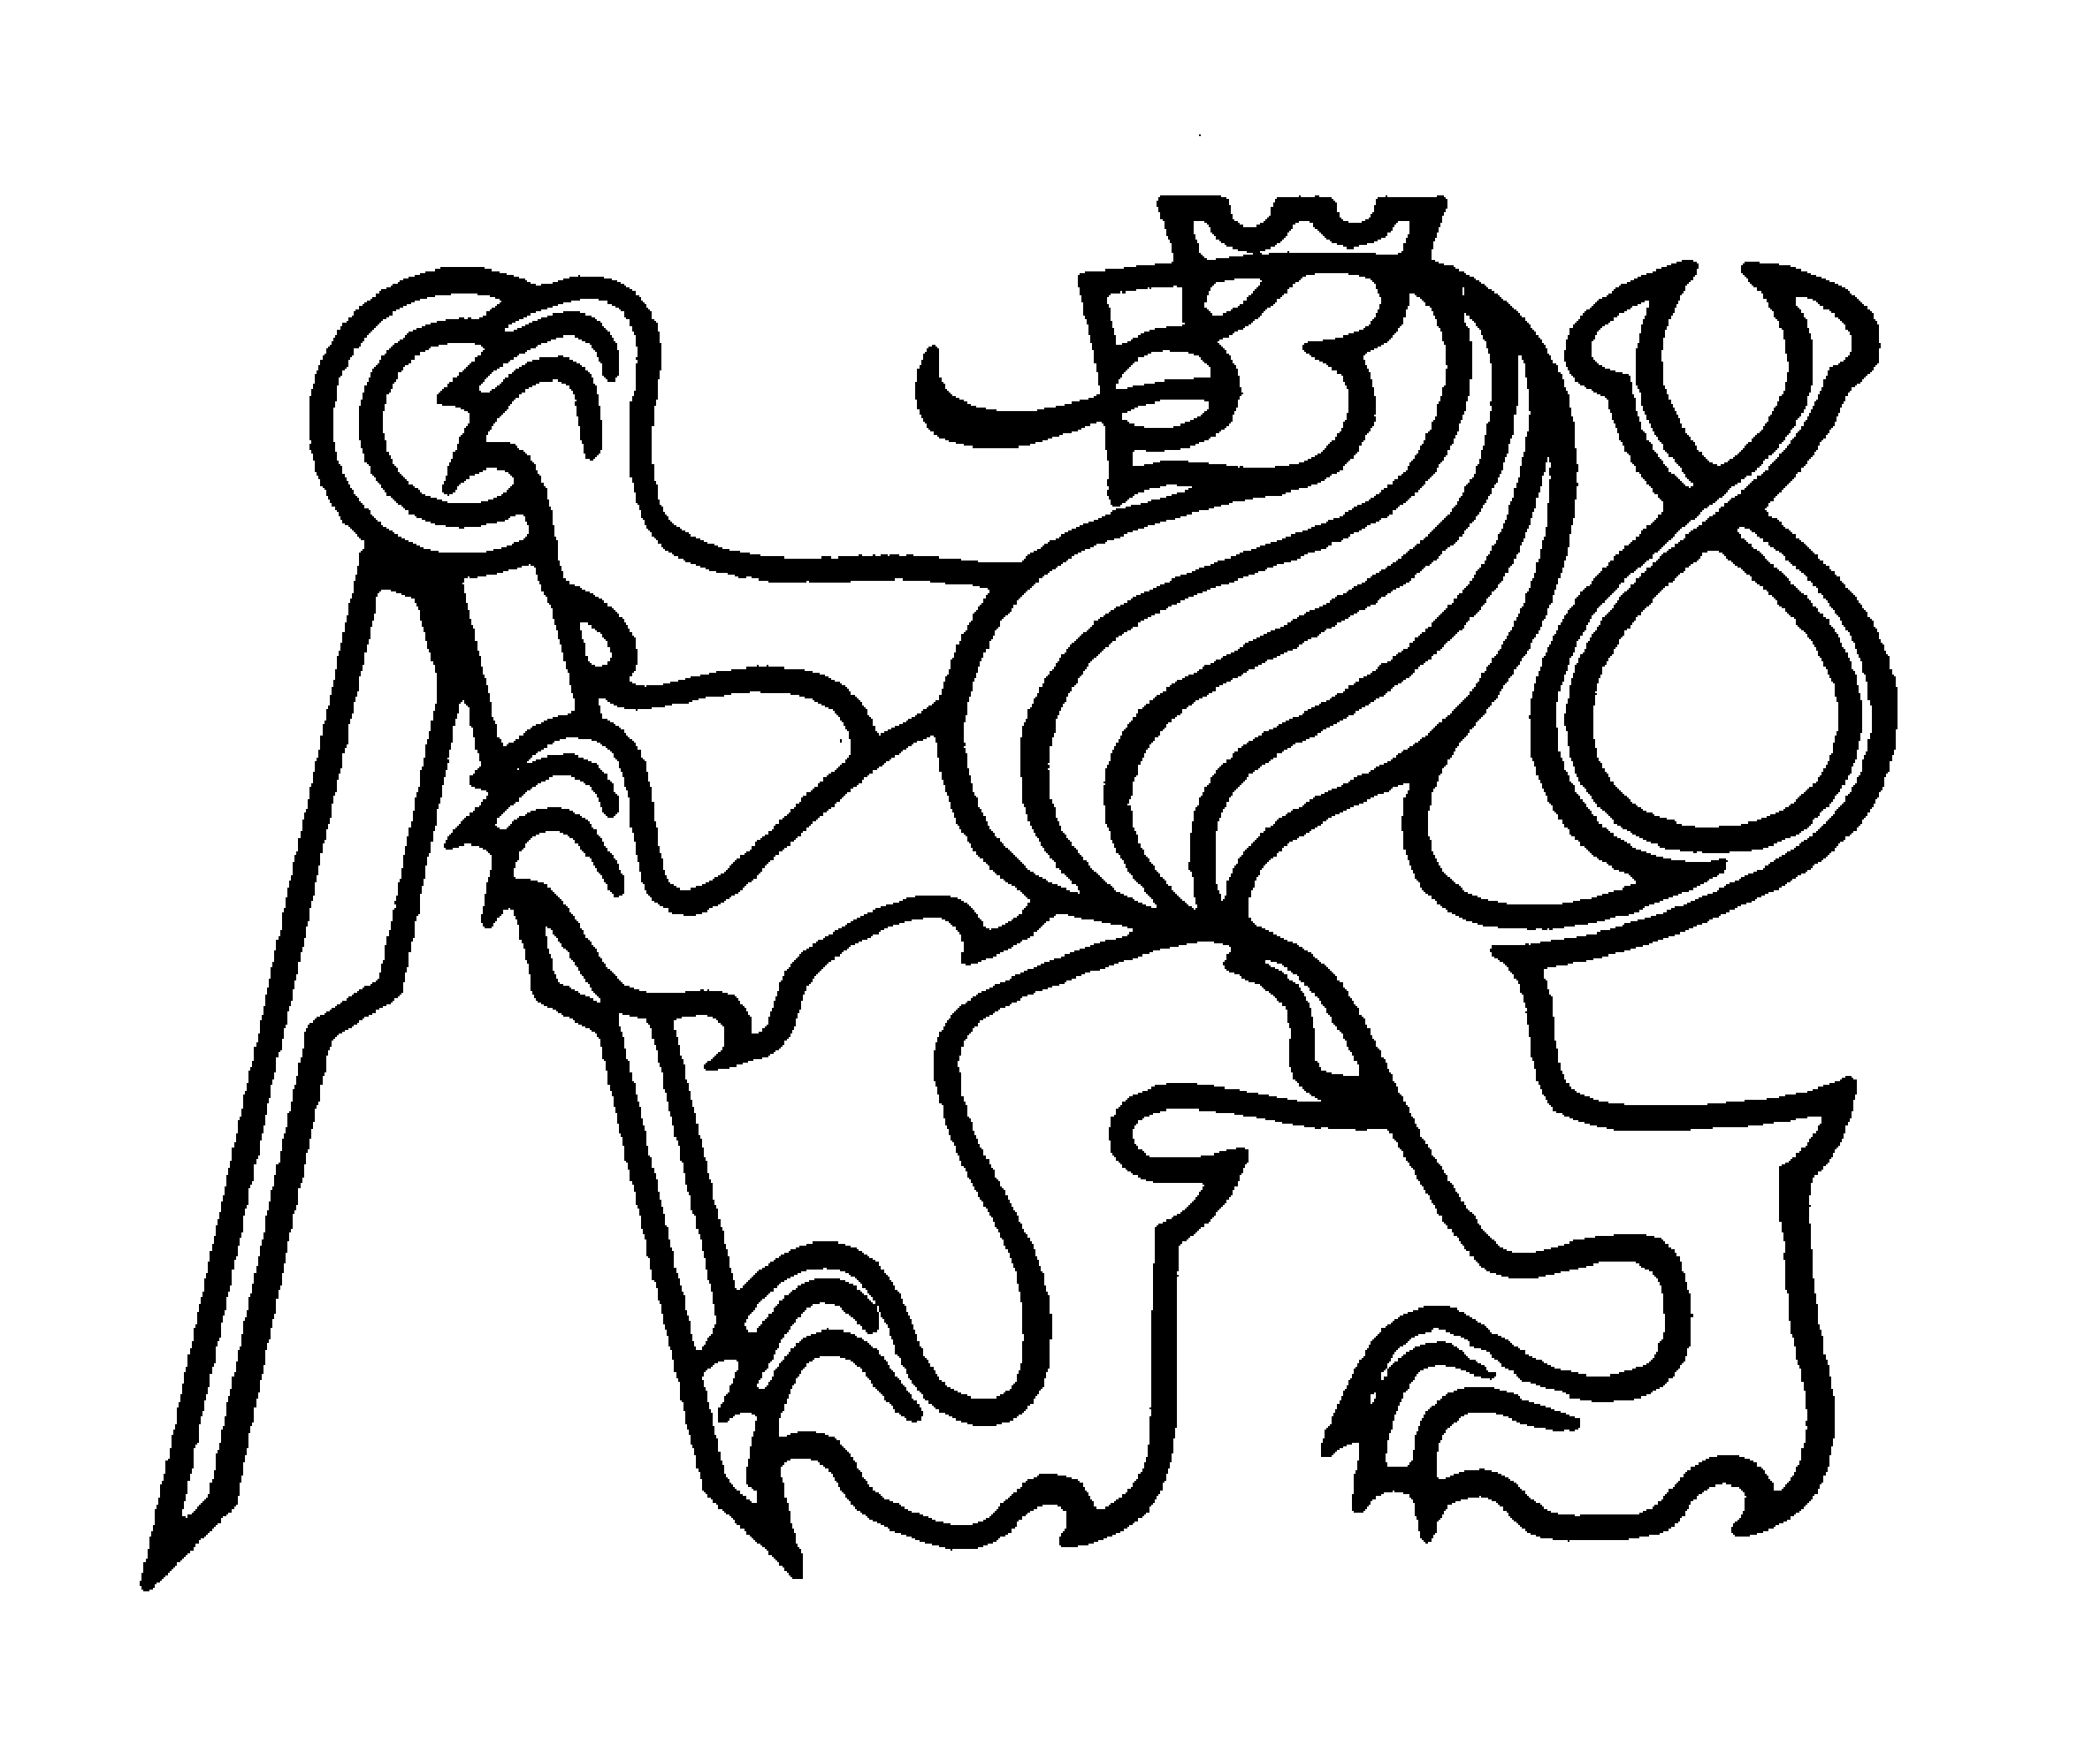
\includegraphics[width=3cm,height=3cm,keepaspectratio]{Images/TITLE/cvut}
\par\end{center}%
\end{minipage}%
\begin{minipage}[c]{0.6\linewidth}%
\begin{center}
\textsc{\large{}Czech Technical University in Prague}{\large{}}\\
{\large{}Faculty of Nuclear Sciences and Physical Engineering}
\par\end{center}%
\end{minipage}%
\begin{minipage}[c]{3cm}%
\noindent \begin{center}

\includegraphics[width=3cm,height=3cm,keepaspectratio]{Images/TITLE/fjfi}
\par\end{center}%
\end{minipage}
\par\end{center}

\vspace{3cm}


\begin{center}
  \textbf{\huge{}Biomarker Analysis of Psychiatric Patients using EEG Signal Analysis and Machine Learning}
\par\end{center}{\huge \par}

\vspace{1cm}


\selectlanguage{czech}%
\begin{center}
\textbf{\huge{}Analýza biomarkerů psychiatrických pacientů pomocí analýzy EEG signálu a strojového učení}
\par\end{center}{\huge \par}

\selectlanguage{american}%
\vspace{2cm}


\begin{center}
{\large{}Diploma thesis}
\par\end{center}{\large \par}

\vfill{}

\begin{lyxlist}{MMMMMMMMM}
\begin{singlespace}
\item [{Author:}] \textbf{Miroslav Kovář}
\item [{Supervisor:}] \textbf{M.Sc. M.A. Sebastián Basterrech, Ph.D.}
\end{singlespace}

% \item [{Language~advisor:}] \textbf{Mgr. Jméno Učitelky Angličtiny}
\begin{singlespace}
\item [{Academic~year:}]2018/2019\end{singlespace}

\end{lyxlist}
\newpage{}

~\newpage{}

~

\vfill{}


\begin{center}
- Zadání práce -
\par\end{center}

\vfill{}


~\newpage{}

~

\vfill{}


\begin{center}
- Zadání práce (zadní strana) -
\par\end{center}

\vfill{}


~\newpage{}

\noindent \emph{\Large{}Acknowledgment:}{\Large \par}

\noindent Some acknoledgment here.

\vfill

\noindent \emph{\Large{}Author's declaration:}{\Large \par}

\noindent I declare that this research project is entirely
my own work and I have listed all the used sources in the bibliography.

\bigskip{}


\noindent Prague, \documentdate\hfill{}Miroslav Kovář

\vspace{2cm}


\newpage{}

~\newpage{}

\selectlanguage{czech}%
\begin{onehalfspace}
\noindent \emph{Název práce:}

\noindent \textbf{Analýza biomarkerů psychiatrických pacientů pomocí analýzy EEG signálu a strojového učení}
\end{onehalfspace}

\bigskip{}


\noindent \emph{Autor:} Miroslav Kovář

\bigskip{}


\noindent \emph{Obor:} Aplikace přírodních věd \bigskip{}


\noindent \emph{Zaměření:} Matematická informatika

\bigskip{}


\noindent \emph{Druh práce:} Diplomová práce

\bigskip{}


\noindent \emph{Vedoucí práce:} M.Sc. M.A. Sebastián Basterrech, Ph.D.,
Artificial Intelligence Center, FEE, CTU Prague

\bigskip{}


% \noindent \emph{Konzultant:} doc. RNDr. Jméno Konzultanta, CSc., pracoviště
% konzultanta. Pouze pokud konzultant byl jmenován.

\bigskip{}


\noindent \emph{Abstrakt:} \bigskip{}


\noindent \emph{Klíčová slova:} 

\selectlanguage{american}%
\vfill{}
~

\begin{onehalfspace}
\noindent \emph{Title:}

\noindent \textbf{Biomarker Analysis of Psychiatric Patients using EEG Signal Analysis and Machine Learning}
\end{onehalfspace}

\bigskip{}


\noindent \emph{Author:} Miroslav Kovář

\bigskip{}


\noindent \emph{Abstract:} 

\bigskip{}


\noindent \emph{Key words:} 

%keywords in alphabetical order separated by commas

\newpage{}

~\newpage{}

\pagestyle{plain}

\tableofcontents{}

\newpage{}


\chapter*{Introduction}
Depression is one of the most common brain disorders - it affacts 121-300 million people worldwide, and this number is expected to increase in the future \cite{rodriguez2015} \cite{whodepression}. Although effective treatments are known, World Health Organization estimates that fewer than half of those affected receive those treatments. Major barriers include insufficient resources, lack of properly trained practitioners, inaccurate assessment and misdiagnosis. \cite{whodepression} 

For these reasons, it is important that affordable, fast, accurate, and easy to use methods for its diagnosis are developed. Although electroencephalography (EEG) \footnote{In this work, we will use the same abreviation for electroencephalography (recording method) and electroencephalographam (the recorded data) where the distinction is apparent from the context.} may be one such method thanks to its comparatively low-cost and easy recording process, comparatively little research has been focused on this area. Non-linear dynamical analysis in particular has been proven very effective at diagnosing mental disorders, and this work is aimed at contributing to this important and relatively new topic.

In \textbf{Chapter 1}, we present some of the classical theory and methods of non-linear dynamical analysis and chaos theory, with focus on the terms used in the following text.

In \textbf{Chapter 2}, we introduce the basic concepts and terminology used in design and evaluation of convolutional neural networks.

In \textbf{Chapter 3}, we describe the methods proposed, experiments performed, and results obtained.

% \addcontentsline{toc}{chapter}{Introduction}

\chapter{Non-linear time series analysis}
The nature is constantly undergoing change. Around us, we can observe many processes evolving in time. Some of the aspects of these processes, we can measure, and attempt to discover apparent patterns in those measurements. The most simple of those patterns are periodicities, probably best exemplified, and first noticed by humans, are the motions of the sun and the moon. Weather, on the other hand, is an example of processes seemingly defying any simple description.

Those examples represent two classes of processes existent before the rise of non-linear dynamics: \cite{andreas2000}
\begin{description}
  \item[Deterministic process]: periodic (or quasi-periodic), fully describable by its Fourier spectrum.
  \item[Stochasitc process]: influenced by forces unpredictable under all circumstances.
\end{description}
Non-linear dynamical analysis studies a third class of processes, which are irregular, non-periodic, yet still deterministic. Every non-periodic, deterministic process is non-linear (bot not necessarily the other way around). Existence of these processes was known already in mid-19th century to J. C. Maxwell, but the field began to be developed only with the rising feasibility of numerical simulations, peaking in 1980s. \cite{andreas2000}

\section{EEG signal}
Electroencephalography (EEG) is a noninvasive method of measuring fluctuations of electric potentials near the skull caused by synchronized firing of neurons in the upper cortical layers. Electroencephalogram is a record of these fluctuations measured over a period of time. \cite{nunez2006}

Although EEG has significantly lower spatial resolution in comparison with other diagnostic techniques such as functional magnetic resonance sampling (fMRI) and magnetoencephalography (MEG) \cite{srinivasan1999} and enables measuring only neural activity near the cortical surface, as a depression diagnostic tool, it has numerous benefits. Importantly, its significantly lower costs \cite{vespa1999} \cite{hamalainen1993}, high portability, and ease of operation imply increased availability to the patients \cite{schultz2012}. Moreover, it is perfectly noninvasive, which means less complications such as claustrophopia or anxiety \cite{murphy1997}.

Although the science of EEG signal analysis as a diagnostic tool brings compelling clinical promise as a result of the aforementioned benefits, it also presents multiple technical and conceptual challenges. 

\begin{figure} 
\centering
\noindent\makebox[\textwidth]{%
  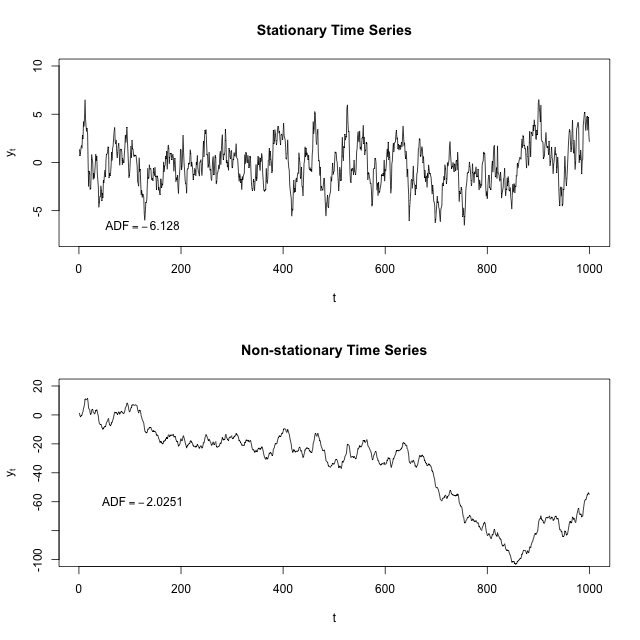
\includegraphics[width=0.8\textwidth]{Images/stationarycomparison.png} }
  \caption{A comparison of stationary and non-stationary time series. (Courtesy: Protonk)}
\label{fig:statnonstatcomp}

\end{figure}
\begin{dfn}[\cite{priestley1988}]
  A series $\{X_t\}_{t \in \ZZ}$ is called \textbf{stationary}, if $\{X_t\}_{t \in \ZZ}$ for any set of times $t_1, t_2, \dots, t_n$ and any $k \in \mathrm{N}$, $P[X_{t_1}, X_{t_2}, \dots, X_{t_n}] = P[X_{t_1+k}, X_{t_2+k}, \dots, X_{t_n+k}]$, i.e. the joint probability distribution of $\{X_t\}_{t \in \ZZ}$ is not a function of time. It is called \textbf{non-stationary}, if it is not stationary.
\end{dfn}

\begin{dfn}[\cite{bickel1996}]
   A series $\{X_t\}_{t \in \ZZ}$ is called (noisy chaotic) \textbf{non-linear}, if it satisfies the relation
   \begin{align}
     X_t = f(X_{t-1}) + \epsilon_t
   \end{align}
   for a general $f : \RR \rightarrow \RR$.
\end{dfn}

EEG signals are prone to be infected with \emph{noise} due to imperfect isolation from surrounding environment. They are known to be \emph{transient, non-Gaussian, non-stationary and nonlinear} \cite{kaplan2005} \cite{stam2005}. Since some patterns do not activate relative to a stimulus, a successful classifier must be able to detect a pattern \emph{regardless of its starting time}, or find one. And finally, EEG records are relatively high dimensional - 16 electrodes sampling at 256 Hz result 4096 data points par second.

Moreover, due to the phenomenon of neural oscillations, patterns may appear in multiple frequency bands, from slow cortical potentials of $\delta$-waves at 0.5-4 Hz, to high $\gamma$ frequency band at 70-150 Hz. 

Patterns of oscillatory activity in various frequency band have been linked to various mental states \cite{canolty2006} \cite{buzsaki2004} and diseases such as epilepsy \cite{shusterman2008}, tremor \cite{mcauley2000}, Parkinson's disease and depression \cite{llinas1999}. Many of the diseases, including depression, share common oscillatory patterns known as thalamocortical dysrythmia, characterized by descrease in normal resting-state $\alpha$ (8-12 Hz) activity slowing down to $\theta$ (4-8 Hz) frequencies, accompanied by increase in $\beta$ and $\gamma$ (25-50 Hz) activity. \cite{vanneste2018}

\section{Limitations in application to EEG}

Some authors suggests that the since most plausible research target for explaining the brain dynamics are the assemblies of coupled and synchronously active neurons, and since majority of those assemblies are describable by non-linear differential equations, principles derived from nonlinear dynamics are applicable to characterization of these neuronal systems. \cite{kaplan2005} 

The approach of estimating a finite embedding dimension, however, has been doubted by some of the most prominent figures in the field of non-linear dynamical analysis, such as the originators of Grassberger-Procaccia algorithm. There is very little evidence for the seemingly improbable hypothesis that such complex system with many extrinsic influences and interactions, such as the brain, would exhibit a level of comlexity comparable to e.g. a Lorenz system. Presumably, the the observed estimates of low dimension are due to artifacts or limited data size. \cite{grassberger1986climatic} \cite{procaccia1988complex}. However, as we will see in Section \ref{sec:applications}, the techniqes derived from these theories still provide some useful information and are successfully applied in many practical situations. Therefore, it seems to be the case that indeed, brain dynamics are much more complex than we are forced to assume based on the theory, but non-linear dynamical analysis still manages to capture some of its important aspects.

\section{Dynamical systems} \label{sec:dynamical-systems}

\begin{dfn}[\cite{andreas2000}]
  Assume that state of a system can be fully described by a finite set of $d$ variabes, such that each state corresponds to a point $\xi \in M$, where $M$ is a $d$-dimensional differentiable manifold. Then we will call $M$ a (true) \textbf{state space} or, equivalently, a (true) \textbf{phase space}, and $d$ its (true) \textbf{dimension}.
\end{dfn}

Although in this study, we will only consider Euclidean $M$, the true state space is needs not necessarily be Euclidean. For example, if some of the state variables are angles, the state space exhibits toroidal topology. However, any topological manifold is locally Euclidean \cite{lee2010introduction} and, since, in EEG signal analysis both $M$ and $d$ are unknown, we have no alternative but to work in Euclidean $M$.

\begin{dfn}[\cite{andreas2000}]
  Let $\xi : \RR \rightarrow \RR^d$ be an $d \in \NN$ dimensional state (phase) space vector dependent on time, and $\mathbf{F}$ a smooth vector field in $\RR^d$. A \textbf{deterministic dynamical system}\footnote{In this work, we are going to assume that brain is a deterministic dynamical system, and that any stochastic component is small and does not change non-linear properties of the system. Thus, by the term dynamical system, we will always mean a deterministic dynamical system.} is described by a set of $d$ first-order differential equations
  \begin{align*}
    \frac{d}{dt}\xi(t) = \mathbf{F}(\xi(t)), \qquad t \in \RR^+_0,
  \end{align*}
  such that there exists a mapping $f^t : M \rightarrow M$ satisfying \footnote{This condition is equivalent to satisfaction of the assumptions of the uniqueness theorem of differential equations.}
  \begin{align*}
   \xi(t) = f^t(\xi(0)).
  \end{align*}
  We will call this mapping \textbf{state evolution function}, and vector field $\mathbf{F}$ \textbf{dynamics of the system}. We call the system linear if $\mathbf{F}$ is a linear vector field.
\end{dfn}

In late 1800s, H. Poincare developed a geometric approach to analyzing the stability (asymptotic evolution) of these systems via examination of the solution $(\xi_1(t), \xi_2(t), \dots, \xi_d(t))$ as a \emph{trajectory} in the phase space $M$ (assuming the solution is known, e.g. measured). These ideas were later extended into deeper understanding of chaos in dynamical systems. \cite{strogatz1996nonlinear} 

In general, any system with temporally changing state is dynamic. A \emph{deterministic} dynamical system is describable by a model giving precise transition of a system from one state to another in time. This means that total description of system's evolution in its phase space (its \emph{trajectory}) is given by the initial state and a set of equations $\mathbf{F}$ (if $\mathbf{F}$ satisfies certain reasonable properties given by the uniqueness theorem). With \emph{stochastic} dynamical systems, such mapping is not possible, since these transitions are not given precisely.

A non-linear dynamical system is a system where the differential equations describing its dynamics are non-linear. Unlike in a linear system, changes in the initial state of a non-dynamical system are allowed to have a non-linear relationship to the state space trajectory of the system. \cite{kaplan2005}

It is important to note the obvious fact that in the case of EEG signal analysis, it is not possible to measure the true state of the system $\xi(t)$. In fact, the observed variables are only a function of the true state of the system, $s(\xi(t))$ for some (generally non-invertible) measurement function $s: \RR^d \rightarrow \RR^{n}$, where $n \ll d$. Morover, the time between subsequent measurements is limited by a sampling frequency and the values of the variables themselves are taken and stored with a limited precision.

\add[inline]{Add a few examples (Lorenz, Rossler, Mackey-Glass). Create my own plots instead of reusing.}

\subsection{Nonstationarity} \label{sec:stationarity}
Nonstationarity is a phenomenon which considerably complicates practical analysis of dynamical systems. All the techniques presented in this text assume stationary process, since this assumption is a prerequisite to deterministic chaos. \cite{isliker1993test} We will call system \textbf{nonstationary} if the dynamics of the system are influenced by causes lying outside of them (and \textbf{stationary} if the opposity is true). In ergodic theory (study of the invariant measures of dynamical systems), the concept of stationarity is defined more rigorously. However, these definitions are not suited numerical applications. \cite{andreas2000} However, a relevant subset of nonstationary systems can be defined more explicitly:
\begin{dfn}[\cite{andreas2000}]
  A dynamical system is called \textbf{nonautonomous} if its dynamics $\mathbf{F}$ are explicitly dependent on time:
  \begin{align*}
    \frac{d}{dt}\xi(t) = \mathbf{F}(\xi(t), t), \qquad t \in \RR^+_0.
  \end{align*}
\end{dfn}

No reliable tests for nonstationarity in this strong sense exist. There is another common definition of a stationary process (sometimes referred to as weak stationarity). A process is called \textbf{weakly stationary}, if all statistical second-order quantities (like mean, variance, and power spectrum) are independent of the absolute time, and at most function of relative times. \cite{isliker1993test}

This weaker definition employs only linear quantites, and is therefore not strictly suitable for non-linear time series analysis. On the other hand, statistical tests of this property exist. In this text, we use the following test discussed by H. Isliker and J. Kurths in \cite{isliker1993test}.

This technique attempts to approximate a projection of so called \emph{physical invariant measure} $\rho$ defined as \cite{eckmann1985ergodic}
\begin{align*}
  \rho  \coloneqq \lim_{T \rightarrow \infty} \frac{1}{T} \int_0^t \delta_{\mathbf{x}(t)} \diff t
\end{align*}
into one coordinate of the state space (given by the time series). Loosely speaking, this measure quantifies ``how often'' are different subsets of the state space visited over infinite time. In other words, it gives a probability that a randomly chosen point on a trajectory will happen to belong to a given subset ``after enough time passed''.
\info[inline]{This measure is related to computation of correlation dimension. Mention it in corresponding section.}

Since this measure is ergodic \footnote{This means, loosely, that it is ``decomposable'' into several different pieces, each again invariant.}, the ergodic theorem basically states that the space and time averages are equal almost everywhere, i.e.
\begin{align*}
  \int_{\mathrm{state space}} f(\mathbf{x}) \rho(\diff \mathbf{x}) = \lim_{T \rightarrow \infty} \frac{1}{T} \int_0^T f(\mathbf{x}(t)) \diff t
\end{align*}
for any $f \in C$ defined on the state space. 

Let $x_1$ represent the measured quantity, and $N$ be the length of the time series. The range of the time series is divided into $K$ intervals $[ x_1^{(k)}, x_1^{(k+1)} ]$, $k=1, 2, \dots, K$., such that the interval boundaries are K-quantiles of the distribution of the values of the time series (i.e. application of the quantile function of the distribution to the values $1/K, 2/K, \dots, (K-1)/K$) \unsure{Is this confusing? Should I just say that they intervals are ``equiprobable''?}, and the number of values falling into each of those intervals is counted:
\begin{align*}
  n_k &\coloneqq \# \{ x_1^{(k)} \leq x_1 \leq x_1^{(k+1)} \} \\
  &\approx \sum_{x_1} \int_{x_1^{(k)}}^{x_1^{(k+1)}} \delta(x-x_1) \diff x \\
  &= \sum_{x_1} \chi_{[x_1^{(k)}, x_1^{(k+1)}]}(x_1),
\end{align*}

where $\xi_{[a,b]}$ is the characteristic function of the set $[a,b]$. The density over the entire series is then approximated by a histogram with $K$ bins as
\begin{align*}
  p_k^{\mathrm{all}} = \frac{n_k^{\mathrm{all}}}{\sum_k n_k^{\mathrm{all}}}.
\end{align*}

If the system is stationary, then the distribution for the first half of the time the same. Hence, this distribution (with the same intervals) is computed for the first half of the time series ($n_k^{\mathrm{half}}$). Then, the two probability distributions are compared using the $\xi^2$-test:
\begin{align*}
  \chi^2 \coloneqq \sum_k \frac{(n_k^{\mathrm{half}} - Zp_k^{\mathrm{all}})^2}{Zp_k^{\mathrm{all}}},
\end{align*}
where $Z = \ceil{N/2} = \sum_k n_k^{\mathrm{half}}$. \cite{isliker1993test}

\section{Attractor} \label{sec:attractor}
Depending on the properties of $\mathbf{F}$, there are several possibilities of how the system might evolve when as $t \rightarrow \infty$. In the following, we will focus on so called dissipative dynamical systems.
\begin{dfn}[\cite{kantz2004}]
  A dynamical system is called dissipative, when it is the case that
  \begin{align}
    E[\mathrm{div} \mathbf{F}] < 0,
  \end{align}
  where the expectation is taken over the state space $M$. In other words, average state space volume of a set of initial conditions of non-zero measure is contracted as the system evolves. 
\end{dfn}

For these systems, after sufficient passage of time, all future states will continue evolving on a bounded, time-invariant subset of $M$. This subset is a geometrical object called an \textbf{attractor}. Example of four basic attractors can be seen on Figure \ref{fig:attractors}.

\begin{figure} 
\centering
\noindent\makebox[\textwidth]{%
  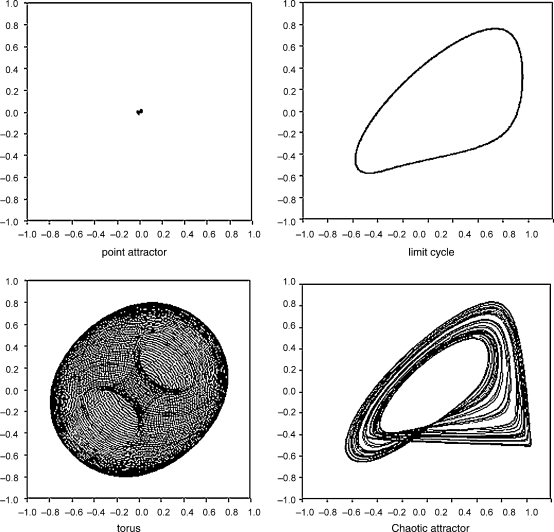
\includegraphics[width=0.8\textwidth]{Images/attractors.png} }
  \caption{Visualization of four common attractor types (units are arbitrary). Left to right, top to bottom:
    \textbf{Point attractor} is the only type of attractor of linear deterministic dissipative systems. It consist of a single final state to which all points from the corresponding region of attraction evolve to.
    \textbf{Limit cycle} corresponds to a periodic dynamical system. It is formed by set of states visited periodically, consituting a trajectory through the state space.
    \textbf{Torus attractor} corresponds to a quasi-periodic dynamical system, resulting (in this example) from a superposition of two periodic oscillations.
    \textbf{Chaotic} (strange) \textbf{attractor}, characteristic of dynamical systems with extending (instead of shrinking) volumes in \emph{some} directions. Corresponding dynamical system may appear stochastic, yet still is completely deterministic. \cite{andreas2000} (\cite{stam2005})}
\label{fig:attractors}
\end{figure}

Since most physiogenerated signals are chaotic, their analysis is concerned primarily with \emph{chaotic} (strange) \emph{attractors}. These attractors are relatively complex, characteristic of dynamical systems with extending volumes in some directions. This property results fast divergence of two initial states, one of which has nonzero component in the direction of growth, i.e. sensitive dependence on the initial conditions. However, since atractors are bounded, the divergence eventually stops and the two trajectories fold together. This continuous expansion and folding may create an attractor with a \emph{fractal structure} (an example of such an attractor is shown on Figure \ref{fig:self-similarity}). \cite{andreas2000} For our purposes it is sufficient to say that this means that these attractors can be characterized as having (quantifiable) self-similarity.\footnote{Cantor set being a canonical example of self-similarity.} However, the following definition related to fractals will be useful in Section \ref{sec:embedding}:
\begin{dfn}[\cite{falconer2004}] \label{def:box-counting}
  Let $F$ be any non-empty bounded subset of $\RR^n$, and let $N_\epsilon(F)$ be the smallest number of sets of diameter at most $\epsilon$ which can cover $F$. Then, the \textbf{box-counting dimension} (also known as Minkowski–Bouligand dimension) is defined as
  \begin{align} \label{eq:box-counting}
    d_0(F) = \lim_{\epsilon \rightarrow 0} -\frac{\log N_\epsilon(F)}{\log{\epsilon}} \, ,
  \end{align}
  if it exists.
\end{dfn}

Intuitively, the number of mesh cubes of side $\epsilon$ intersecting $F$ gives an indication about how irregular the set is when inspected at scale $\epsilon$, and the box-counting dimension reflects ``how rapidly'' the irregularities develop as $\epsilon \rightarrow 0$. \cite{falconer2004} 

\begin{figure} 
\centering
\noindent\makebox[\textwidth]{%
  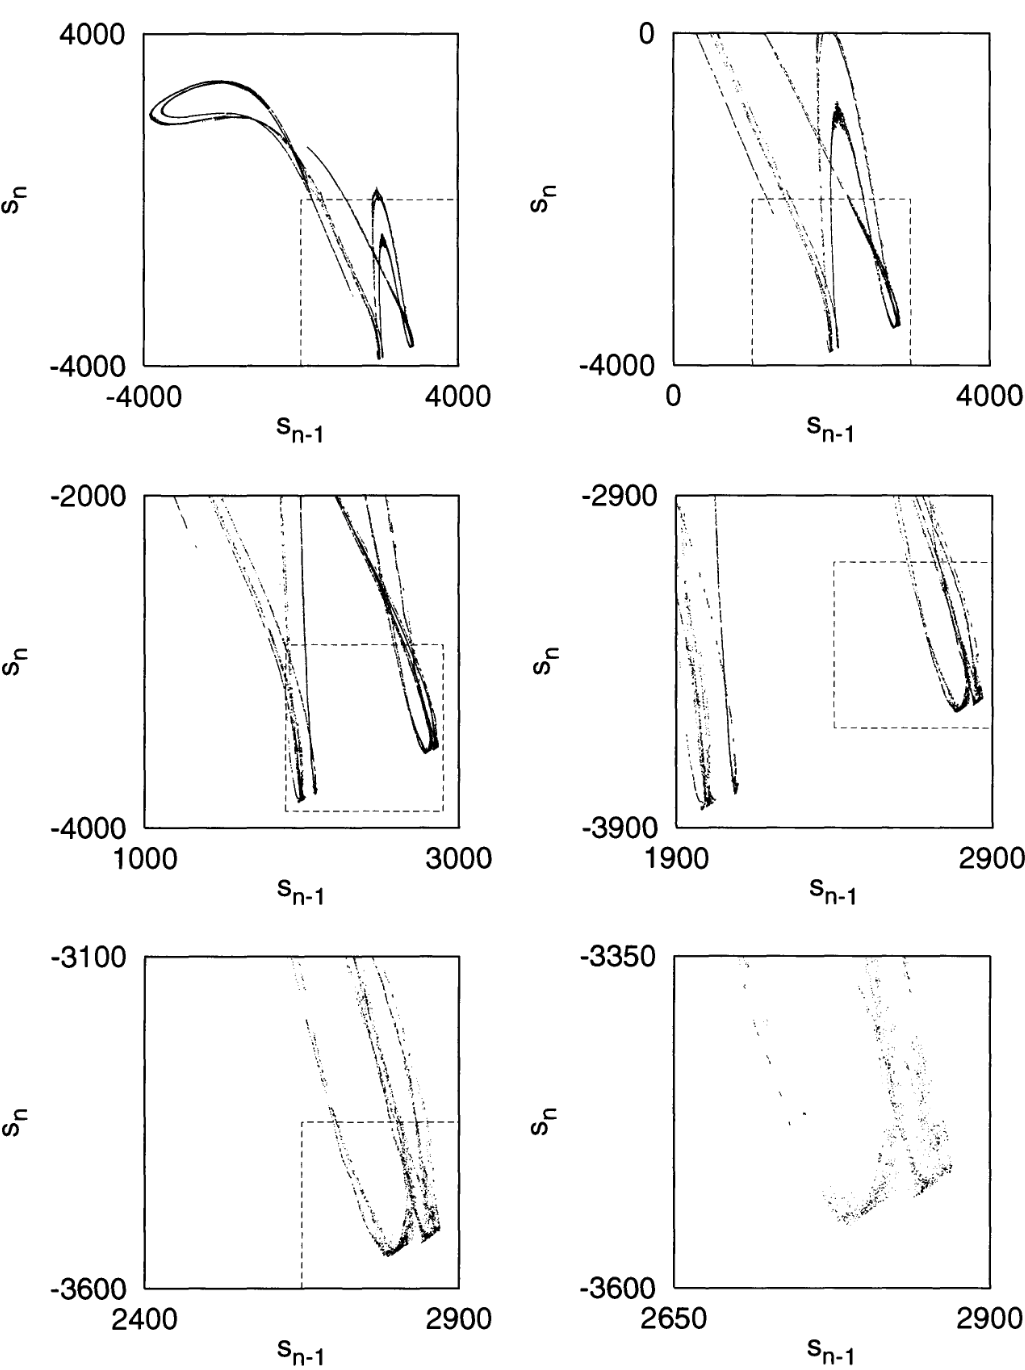
\includegraphics[width=0.8\textwidth]{Images/self-similarity.png}}
  \caption{Noise-reduced visualization of successive enlargements of highly self-similar attractor. (\cite{kantz2004})}
\label{fig:self-similarity}
\end{figure}

\section{State space reconstruction} \label{sec:state-space-reconstruction}

Broadly, one possible approach to non-linear time series analysis consists of the following steps: 
\begin{enumerate}
  \item reconstruction of the attractor \info{Saying dynamics is not true. We are not reconstructing the vector field $\mathbf{F}$.} of given system from recorded data,
  \item characterization of the reconstructed attractor,
  \item checking validity of the results with surrogate data testing. \cite{stam2005}
\end{enumerate}

\add[inline]{Connect this to the content of this section. Expand on the steps.}

\subsection{Embedding} \label{sec:embedding}
In the previous section, we have introduced a concept of state space of a dynamical system. In the case of EEG analysis, however, our observations do not directly form a state space object, but a set of time series (a sequence of scalar measurements), one for each electrode. Moreover, it is necessary to deal with the fact that our data, however rich, rarely represent complete information about the studied system. In the case of EEG signals, the complete state of the system at any moment is determined by many variables, and the sensors are only able to collect traces of their cumulative effects (and noise). So we are confronted with a problem: how to convert this data into state space trajectories? This procedure is called \emph{state space reconstruction}.

To this goal, let $\mathbf{s}_n$ be the reconstructed vector we are trying to find, and let us have a time series of scalar measurements of a quantity depending on the current state of the system:
\begin{align} \label{eq:measurements}
  x_n = s(\xi(n \Delta t)) + \eta_n(n \Delta t) \, ,
\end{align}
where $\xi$ is a state space vector, $s(\cdot)$ is a measurement function and $\eta_n$ is a measurement noise. Furthermore, let us consider a function $\Phi: M \rightarrow \RR^m$, such that $\mathbf{x}_n = \Phi(\xi(n \Delta t))$. Such function is called an \textbf{embedding}. In the following, we will discuss what properties does $\Phi$ have to satisfy so that it provides useful information about the true state space trajectories.

Before we do that, let us mention the following. As we have stated in Section \ref{sec:dynamical-systems}, our observations are formed by application of non-invertible measurement function $s: \RR^d \rightarrow \RR^{d'}$, $d' \ll d$, to the true states of the system. Aside from being a projection, $s$ may be also be a distortion. Therefore, it might seem impossible to reconstruct the true state space trajectory and this indeed may be the case in some situations. On the other hand, there are quantities invariant under distortion which may be preserved. \cite{andreas2000} Moreover, if our goal was to study only the attractor properties, perfect reconstruction may not even be desirable in the case that the attractor dimension is smaller than the dimension of the original space \cite{kantz2004}.

Firstly, note that we assume the studied dynamical system to be deterministic. If our reconstructed embedded space is to represent the true state space, evolution of any state on every trajectory we observe in the embedded space should depend only on its current state. Therefore, we may reasonably require $\Phi$ to be one-to-one, i.e. contain no intersections.

Secondly, since many of the attractor properties we care about (such as correlation dimensions, Lyapunov exponents, etc.) are only invariant under smooth non-singular transformations, in order to preserve these properties in the embedded space, we may require $\Phi$ to preserve the differential structure of the state space $M$. This corresponds to the tangent space $D \Phi$ also being a one-to-one mapping. 

\add[inline]{Add images illustrating these two conditions.}

\subsection{Method of time delays} \label{sec:method-of-delays}
There are two common approaches to the problem of state space reconstruction for EEG time series data:
\begin{description}
  \item [Time delay embedding]: state space is reconstructed separately for each time series.
  \item [Spatial embedding]: each time series corresponds to a coordinate of the state space vector.
\end{description}

Int the following text, we will focus on the first one, because we are not using the second one in this thesis, and it has been widely criticised. \add{Add some citations.}

It had been already known since 1936, that every $n$-dimensional differentiable manifold can be embedded in $\RR^{2n+1}$, and that the set of such embeddings is open and dense in the space of generic smooth maps, which is known as Whitney's theorem. \cite{whitney1936} \footnote{The second part of the theorem is a consequence of the fact that two hyperplanes with dimensions $d_1$ and $d_2$ in $m$-dimensional space are likely to intersect if $d_1 + d_2 \geq m$.}) In other words, $2n+1$ independent measurements of a $n$-dimensional system can be uniquely mapped to a $2n+1$ dimensional space, hence each such $2n+1$ dimensional vector identifies identifies state of the system perfecly, thus reconstructing the true state space.

Time delay embedding is a technique of state space reconstruction, which achieves the same goal, but with a single measured quantity. It was first introduced into the field of non-linear dynamical system analysis by N. H. Packard in 1980 (although it was already being used in different fields in 1950s \cite{andreas2000}). Studying the Rossler system, Packard noticed that by sampling a single coordinate, he was able to obtain a faithful phase-space representation of the original system by simply using a value of a coordinate with its values at two previous times. \cite{packard1980} In other he demonstrated numerically that past and future measurements of one variable contain information about the unobserved variables and can be used to define the present state.

In particular, for each time $t$, we define an embedding window $\tau_w$, and use measurements obtained at times $t'$ for $t-\tau_w \leq t' \leq t$. To this goal, we use $m$ measurements, $\tau$ elements apart. Here, $\tau$ is called \emph{lag} or \emph{time delay}, and is measured in number of samples\footnote{Some authors use the time units $\tau \Delta t$, where $\Delta t = t_s = 1/f_s$ is the sampling period.}. Using the notation of \ref{eq:measurements}, the time delay reconstruction is then formed by the following vectors:
\begin{align}
  \textbf{x}_n = (x_{n-(m-1)\tau}, x_{n-(m-2)\tau},\dots,x_{n-\tau}, x_n) \, ,
\end{align}
for $n > (m-1)\tau = \tau_w$. \cite{kantz2004} 

A year after Packard's discovery, in \cite{takens1981}, F. Takens has proved theoretically that the attractor reconstructed using this method may have the same dynamical properties (entropy, dimension, Lyapunov spectrum) as attractor of the original system under some conditions. Takens delay embedding theorem is an important result of non-linear time series analysis and can be stated as follows:
\begin{thm}[\cite{takens1981}] \label{thm:takens}
  Let $M$ be a compact\footnote{This theorem can be proved for $M$ non-compact provided less restrictions are imposed on $s$.} smooth manifold specifying the state space of a deterministic dynamical system of dimension $d \in \NN$, $s : M \rightarrow \RR^n, s \in C^2$ a smooth measurement function, $f^t : M \rightarrow M, f \in C^2$ a set smooth diffeomorphic state evolution functions for $t \in \RR$. Then the set of maps $\phi_{(s,f^t)} : M \rightarrow \RR^{2d+1}$, defined by
  \begin{align}
    \phi_{(s,f^t)}(x) = (s(\xi), s(f^{-\tau}(\xi)), \dots, s(f^{-2d\tau}(\xi))),
  \end{align}
  for which $\Phi$ is an embedding is an open and dense set in the space of maps satisfying the assumptions above.
\end{thm}

This idea has a simile in the existence theorems in the theory of differential equations, which say that a unique solution exists for each $x(t), \dot{x}(t), \ddot{x}(t), \dots$. For example, in many body dynamics under Newtonian gravitation, knowledge of a body's position and momentum is sufficient to uniquely determine its future dynamics. \cite{ScholarpediaReconstruction}

Taken's theorem, although of theoretical importance, is not necessarily useful in practice, since even dense sets can have measure zero. Moreover, it is restricted to smooth manifolds. An add came ten years later, when T. Sauer both generalized Takens' result as follows (in a simplified form):
\begin{thm}[Sauer, \cite{sauer1991}] \label{thm:sauer}
  Let $A$ be a compact fractal with box-counting dimension $d_A$, and let $A$ be a subset of a $m$-dimensional manifold. Then
  \begin{align*}
    \lbrace \Phi: A \rightarrow \RR^{m} | \Phi \in C^1, m > 2d_A \rbrace \text{ is an embedding with probability } 1.
  \end{align*}
\end{thm}

In conclusion, Theorem \ref{thm:takens} and Theorem \ref{thm:sauer} together ensure that when $m$ is chosen such that $m > d_A$i (which may be a considerable reduction in dimension compared to $m \geq 2d+1$), then $\Phi$ a true embedding of the underlying attractor for almost any $\tau$ (note only sufficiency of the result - $\textbf{x}_n$ may be an embedding even for smaller $m$).

A fascinating consequence of Theorem \ref{thm:sauer} when applied to a sequence of measurements recorded from a physical system is that a successfully reconstructed attractor does not describe the time series, but the system itself. In the words of Theiler: ``If one believes that the brain (say) is a deterministic system, then it may be possible to study the brain by looking at the electrical output of a single neuron. This example is an ambitious one, but the point is that the delay-time embedding makes it possible for one to analyze the self-organizing behavior of a complex dynamical system without knowing the full state at any given time''. \cite{theiler1990estimating}

\subsection{The effects of noise}
Although these theoretical results are important to know about, they all make practically unrealistic assumptions, such as infinite amount of data and infinite measurement precision, and absence of noise. Moreover, practical applications present further challanges, such as presence of noise.

Several factors complicate successful reconstruction from real-world, experimental data: \cite{casdagli1991state}
\begin{description}
  \item[Observational noise.] Given a reconstructed vector $\mathbf{x} \in \RR^m$, there is a (approximatly Gaussian shaped in natural scenarios) distribution $p(\mathbf{x})$ in the reconstruction space due to the noise term in equation (\ref{eq:measurements}). \cite{andreas2000}
  \item[Dynamic noise (nonstationarity).] External influences perturb the system, which consequently appears nondeterministic.
  \item[Estimation error.] Estimation of the dynamics of the system is performed using only limited amount of data.
  \item[Quantization error.] The measured analogue quantity is converted and stored as a number with only finite number of bits.
\end{description}

Moreover, different reconstructions can amplify the already present noise to varying degree. In \cite{casdagli1991state}, Casdagli et al. provide a quantitative way of analyzing this amplification, and, by extension, of insight into selection of embedding parameters so that the noise amplification is minimized.

\subsection{Time delay selection} \label{sec:delay}
A careful reader might have noted that the results of theorems in Section \ref{sec:method-of-delays} do not depend on the value of the delay $\tau$.\footnote{This is because of the fact that the measurements are infinitely precise. \cite{casdagli1991state}}. Embeddings with the same value of the embedding dimension $m$, but different values of $\tau$ are theoretically equivalent. In practice, however, some theoretically sound time delay reconstructions may fail to be embeddings. Although some researchers propose that the only important parameter is the length of the embedding window $\tau_w = \tau (m-1)$ \cite{kugiumtzis1996state}, as we will see, the choice of time delay has effects independent of the choice of embedding dimension, and vice versa.

For example:
\begin{enumerate}
  \item The embedding may fail to be a one-to-one map due to finite precision, or presence of noise in the data. \cite{andreas2000}
  \item Highly chaotic systems with large Lyapunov exponents (see Section \ref{sec:lyap}) and large dimension, projection to a low dimensional time series causes explosion in the noise amplification. As a result, this imposes limits on short term predictablity and state space reconstruction may become impossible. Such systems should be treated as operationally stochastic. \cite{casdagli1991state}
  \item It was shown that increasing $\tau$ leads to rise in entropy. \cite{Kantz1997}
  \item Deterministic behavior can be observed only when $\tau_w$ is smaller than the time scale of the foldings naturally produced as result of time embedding.
  \item If the values of $\tau$ are \emph{too small} in comparison to the typical time scales of the series (measured e.g. by mean period), then the successive elements of reconstructed state space vectors become almost equal. This effect is often called \emph{redundance}. Since $x_t \approx x_{t + \tau}$, the reconstructed attractor will concentrate along the main diagonal (see Figure \ref{fig:delay}, left hand side). Moreover, in this case, the effect of noise is amplified. \cite{casdagli1991state}
  \item If the values of $\tau$ are \emph{too large}, the successive elements in the reconstructed vector are almost independent. This effect, called \emph{irrelevance} or \emph{overfolding} is even magnified if the underlying attractor is chaotic, since deterministic correlations between states are lost even at very small time scales, i.e. even measurements performed at time $t$ and $t + \tau$ for very small $\tau$ may be already unrelated. The reconstructed attractor will form a seemingly random clound in $\RR^m$ - thus the reconstructed attractor may appear complex, even if the true attractor is simple (see Figure \ref{fig:delay}, right hand side). 
\end{enumerate}

In summary, picking the proper value of $\tau$ is a balancing act between redundance and irrelevance. It is important to minimize excessive foldings, and extreme closeness between adjacent points on the trajectory (ideally, the distances between points is same in the reconstructed as in the true space).

\begin{figure} 
\centering
\noindent\makebox[\textwidth]{%
  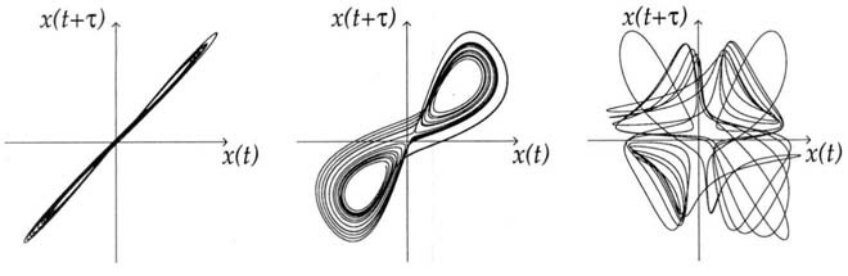
\includegraphics[width=1\textwidth]{Images/delay.png} }
  \caption{Time delay reconstructions of the Lorenz attractor for different values of $\tau$. Figure on the left hand side shows choice of small $\tau$ and represents the case of redundance - the states concentrate along the main diagonal. Figure in the middle shows a successful reconstruction (although not an embedding, for which $m \geq 3$ is required). Figure on the right hand side shows a choice of large $\tau$ and represents the case of irrelevance - the reconstruction lacks apparent structure. (\cite{andreas2000})}
\label{fig:delay}
\end{figure}

\subsubsection{Autocorrelation} \label{sec:acorr}
From the above, we understand that statistical non-correlation between values of coordinates of the reconstructed vectors $\mathbf{x}_n$ are desirable property of a time delay embedding. Thus, a natural method of estimating the optimal time delay is studying the \emph{autocorrelation function} $A$, and picking the first $\tau$ where $A(\tau)$ decays below a threshold value - commonly used are $A(0)/e$ \cite{stam2005}, $1-A(0)/e$ \cite{kantz2004}, or even the first local minimum \cite{albano1993reliability, abarbanel2012analysis} or the first $0$ crossing \cite{kantz2004}.

\begin{dfn}[\cite{kantz2004}]
  \textbf{Autocorrelation} $A : \RR \rightarrow \RR$ for time delay $\tau$ is given by
  \begin{align*}
    % A(\tau) = \frac{1}{\sigma^2} \langle (s_n - \langle s_n \rangle )(s_{n-\tau} - \langle s_n \rangle) \rangle \\
    A(\tau) = \frac{E[(x_i - \overline{x})(x_{i-\tau} - \overline{x})]}{\sigma^2}, 
  \end{align*}
\end{dfn}
where $\overline{x}$ is the mean of the time series, and $\sigma^2$ is its standard deviation.


Computing the autocorrelation function is not only useful for examining the stationarity of the time series, but it also gives a geometrical insight into the shape of the attractor: if we approximate the cloud of reconstructed vectors $\mathbf{x}_n \in \RR^m$ by an ellipsoid, lengths of its semi-axis are given by the square root of the eigenvalues of its auto-covariance matrix. In two dimensions, zero of the covariance matrix corresponds to those eigenvalues being equal, i.e. $x_t$ and $x_{t-\tau}$ being completely uncorrelated. \cite{kantz2004} An obvious objection is that correlation between $x_t$ and $x_{t-\tau}$ says nothing about correlation between $x_t$ and $x_{t-2\tau}$, etc. Thus, this method, since it computes correlations only between two successive coordinates, is generally useful only for low dimensional systems.

Autocorrelation also provides a lower bound for $\tau$ in the following sense. If the data is noisy, vectors formed by time delay embedding procedure are practically meaningless, if the variation of the signal in the time covered in the time window $\tau_w = (m-1)\tau$ is less the the variation of noise. This means that $\tau$ should be selected such that $A(\tau) > A(0) - \sigma^2_{\text{noise}}/\sigma^2_{\text{signal}}$. \cite{kantz2004}

\subsubsection{Delayed mutual information} \label{sec:dmi}
Another commonly used method is to use the first minimum of the \emph{time delayed mutual information}. \cite{fraser1986independent} 

\begin{dfn}[\cite{kantz2004}]
  Let probability density of the values of a time series be split into $\epsilon$-wide histogram bins. Let $p_i$ be the probability that a signal assumes value in $i$-th bin of the histogram, and let $p_{ij}(\tau)$ be the the probability that $x_t$ is in a bin $i$ and $x_{t+\tau}$ is in a bin $j$. \textbf{Delayed mutual information} $\mathcal{I}_{\epsilon}$ for time delay $\tau$ is defined as
  \begin{align*}
    \mathcal{I}_{\epsilon}(\tau) = \sum_{i, j} p_{ij}(\tau) \ln p_{ij}(\tau) - 2 \sum_{i} p_i \ln p_i.
  \end{align*}
\end{dfn}

In other words, time delayed mutual information the average mutual information between measurements obtained by the original time series and its $\tau$-shifted (time delayed) counterpart. The optimal $\tau$ is usually selected as $\argmin_{\tau} \mathcal{I}_{\epsilon}(\tau)$.

Although this approach yields coordinates independent in a more general sense than simple linear independence provided by the autocorrelation function, the same criticism applies: minimum dependence between $x_t$ and $x_{t-\tau}$ says nothing about dependencies between other coordinates. Again, using this method is justifiable only for two-dimensional reconstructions. However, delayed mutual information has been generalized for multiple dimensions by its proponent A. M. Fraser using multidimensional distributions into a concept he called \emph{redundancy}, which basically measures the degree to which the reconstructed vectors accumulate around the bisectrix of the embedding space. \cite{fraser1989reconstructing} 

Another criticism of delayed mutual information that some systems exhibit slowly decaying mutual information which has no minima. \cite{martinerie1992mutual} 

\subsubsection{Average displacement from diagonal}
\textbf{Average displacement from diaognal} is a simple technique which simply measures the average distance of the embedding vectors from their original location:
\begin{align*}
  \mathrm{ADFD}(m, \tau) = \frac{1}{N_{(m, \tau)}}\sum_{i=1}^{N_{(m, \tau)}} \norm{ \mathbf{x}_i^{(m, \tau)} - \mathbf{x}_i^{(m, 0)}},
\end{align*}
where $\mathbf{x}_i^{(m, \tau)}$ is the $i$-th vector of time delay embedding with embedding dimension $m$ and time delay $\tau$.

Rosenstein et al. presented multiple methods for quantifying expansion from the main diagonal, and found $\mathrm{ADFD}$ to be the most computationally efficient, robust to noise, and accurate. \cite{rosenstein1994reconstruction} They also experimentily identified optimal $\tau$ as the one for which the slope of $\mathrm{ADFD}$ drops below 40\% of its initial value.  

\subsubsection{Singular values analysis}
All the approaches described so far address the issue of irrelevance, but not that of redundance. In fact, based mostly on empirical, rather than the most time delay estimation techniques optimize for the following criteria \footnote{However, additional criteria may arise depending on the particular application.}: \cite{kugiumtzis1996state} 
\begin{enumerate}
  \item The reconstructed attractor must be expanded from the diagonal.
  \item The components of the reconstructed vector $\mathbf{x}_n$ must be uncorrelated.
\end{enumerate}

Those criteria are noticeably similar, and bias towards larger estimates of $\tau$. This leads many authors to suggest more advanced techniques, such as generalized delayed mutual information mentioned above, or some of those introduced in the following text.

Principal component analysis, in particular, can be used to measure the volume occupied by the reconstructed attractor. Both overfolded and redundant attractors may be marked by low volume. \cite{andreas2000}

Given a fixed embedding dimension $m$, the corresponding $m$ singular values as a function of $\tau$ contain information about the degree of extension of the embedded vectors in the $m$ directions in the reconstructed space. Rapid increase followed by rapid decrease of some singular values accompanied by the opposite behavior of others indicate a collapse of the attractor. Also, high number of large singular values is an indicator of volume of the reconstructed attractor.

If we assume, without loss of generality\unsure{Is this so?}, that the time series is standardized and denote
\begin{align*}
  \mathbb{X} \coloneqq \begin{pmatrix} \mathbf{x}_1^T \\ \mathbf{x}_2^T  \\ \dots \\ \mathbf{x}_{N_{(m, \tau)}}^T  \end{pmatrix},
\end{align*}
then
\begin{align*}
  (\mathbb{C})_{ij} \coloneqq (\mathbb{X}^T\mathbb{X})_{ij} = A\left( (i-j)\tau \right).
\end{align*}
This matrix is symmetric and thus diagonalizable, and also at least non-negative definite. Its eigenvalues are called the singular values, and correspond the the magnitude of variance of projections of the embedded vectors into individual directions of the principal components.

If the time delay is too small, then all the elements of matrix $\mathbb{C}$ will have similar value $(\mathbb{C})_{ij} \approx A(0)$, and thus there will be one dominant singular value, while others will remain close to zero. This singular value then corresponds to the main diagonal of the attractor.

If the time delay is too large, then the diagonal elements will approach average of the squared time series $(\mathbb{C})_{ii} \approx \langle x^2 \rangle$, while the remaining elements will converge to zero due to decay of the autocorrelation function, $\mathbb{C} \approx c\mathbb{I}$for some constant $c$. This corresponds to the reconstruction forming a featureless noise. \cite{andreas2000}

One drawback of this method is that its evaluation is largely subjective. Moreover, it was suggested that although this method is effective noise reduction technique, its effectiveness at delay estimation is less clear - the number of large singular values is sensitive to noise. \cite{mees1987singular}

\subsubsection{Integral local deformation}
The uniqueness theorem of differential equations requires that any no trajectories in the state space intersect. Moreover, in real physical systems, it may be reasonable to assume that it is highly unlikely to find closeby trajectories of opposite or orthogonal directions. This property is maintained by a successful embedding, and (if the assumption holds) can occur only in an improper reconstruction.

T. Buzug and G. Pfister presented a quantitative measure of these close trajectory intersections by comparing the the evolutions of reference trajectories with centroids of points on the neighboring trajectories. \cite{buzug1992optimal} For the optimal embedding, divergence between these trajectories should be minimized.

First, multiple random reference points are chosen. Let $\mathbf{x}_i(0)$ be such a reference point at time 0. Then, either a fixed number of nearest neighbors or all neighbors within a given radius and their centroid $\mathbf{x}_i^{com}(0)$ are found. Then, the absolute growth of the distance between the centroid of those originally neighboring points and the reference point after $qt_{ev}$ time steps is found as:
\begin{align*}
  \Delta(q,m,\tau) = \norm{\mathbf{x}^{com}(qt_{ev}) - \mathbf{x}_i(qt_{ev})} - \norm{\mathbf{x}_i^{com}(0) - \mathbf{x}_i(0)}.
\end{align*}

The values $\Delta(q,m,\tau)$ are discretely integrated from $q=1$ to $q=q_{max}$:
\begin{align*}
  \mathcal{D}(m, \tau, i) = \frac{t_{ev}}{2} \sum_{q=1}^{q_{max}} \left( \Delta(q-1,m,\tau) - \Delta(q,m,\tau) \right).
\end{align*}
This expression, called \textbf{integral local deformation}, is then averaged over $N_{ref}$ reference points and normalized:
\begin{align*}
  \langle \mathcal{D}(m, \tau, i) \rangle_i = \frac{t_{ev} \sum_{i=1}^{N_{ref}} \sum_{q=1}^{q_{max}} \left( \Delta(q-1,m,\tau) - \Delta(q,m,\tau) \right)}{2N_{ref} \Delta t \left( \max_{i \in 1, 2, \dots, N} x_i - \min_{i \in 1, 2, \dots, N} x_i \right)}
\end{align*}

\subsection{Embedding dimension selection}
\subsubsection{False nearest neighbors} \label{sec:fnn}
Since the dynamics $\textbf{F}$ are assumed to be a \emph{smooth} vector field and the attractor $A$ is a \emph{compact} set in the phase space, its members acquire near neighbors, which should be subject to similar evolution. Therefore, these neighbors should remain close to each other after a short interval of time (even though chaos may introduce exponential divergence between them). This is a useful fact, which can be used, for example, to predict future evolution of a trajectory, or a computation of Lyapunov exponents. The \textbf{false nearest neighbors} algorithm uses them for estimation of embedding dimension. \cite{kennel1992determining}

The main idea is to use the transition from dimension $m$ to dimension $m+1$ in the embedding procedure to differentiate between ``true'' and ``false'' neighbors. If the embedding dimension $m$ is too small, some members of $A$ that are close to each other may not be neighbors in the true state space, simply because the true state space is projected down to a smaller space (see Figure \cite{})\add{Add the figure from Kennel.}. These members are \emph{false neighbors}, all other neighbors are \emph{true}. When the attractor is fully unfolded into large enough dimension and is properly embedded, all neighbors are true.

Let use denote by $y^{(r)}(n)$ the $r$-th nearest neighbor of $y(n)$. Then, let $R_m(n,r)$ denote the Euclidean distance between $y(n)$ and its neighbor:
\begin{align*}
  R_m(n,r) = \sqrt{ \sum_{k=0}^{m-1}[ x_{n+k\tau} - x^{(r)}_{n+k\tau} ]^2 }
\end{align*}

Then, any near neigbor for which the distance increase after transition from dimension $m$ to dimension $m+1$ is large in comparison to the initial distance is marked as false:
\begin{align} \label{eq:first-criterion}
  \left[ \frac{R_m^2(n,r) - R_{m+1}^2(n,r)}{R_m^2(n,r)} \right]^{1/2} = \frac{ x_{n+k\tau} - x^{(r)}_{n+k\tau} }{R_m(n,r)} > R,
\end{align}
where $R \in \RR$ is some threashold. The $m$ for which the relative proportion of false neigbors to all neigbors reaches zero is the embedding dimension suggested by this criterion.

This criterion, by itself, is not sufficient for determining proper embedding dimension. When applied to limited amount of white noise data, it erroneously suggested embedding the noise into a low dimensional attractor. This happens because even though a state may be a nearest neigbor, it is not necessarily temporally close, and thus the assumptions above do not hold. The experiments performed by Kennel et al. show for such states it is usually $R_m(n,r) \approx R_A$, where $R_A$ is radius of the attractor. Furthermore, for increasing amount of data, the embedding dimension suggested by this criterion also increased - behavior not observed for relatively small dimensional attractors. \cite{kennel1992determining} 

Therefore, Kennel et al. propose another criterion in addition to the one above. Since false neighbors which are near, but temporally distant, are usually stretched to the extremeties of the attractor with transition from $m$ to $m+1$, they suggest marking all near neighbors satisfying
\begin{align} \label{eq:second-criterion}
  \frac{R_{m+1}(n,r)}{R_A} > A
\end{align}
as false, where $R_A$ may be computed as, for example 
\begin{align*}
  R_A = \frac{1}{N} \sum_{n=1}^{N} \left[ x_n - \overline{x} \right]^2.
\end{align*}

Although this technique is commonly used, it is not without its drawbacks. An obvious point is that altough it is true that distance between neigbors in unfolded attractor should not grow with increase in dimension, the inverse is not necessarily true, i.e. stable distance between near neighbors with increase in dimension does not guarantee that these neighbors are true. 

The authors suggest some values of the tolerance parameters they found useful in their experiments, but, in general, the results of this technique may depend on the choice of $R$ and $A$. Their selection is subjective and somewhat arbitrary. The best course of action is to evaluate the technique for multiple values of $R$ and $A$ and select those with the most ``reasonable'' results.

In practice, it has been found that the results of this method are sensitive not only to the tolerance parameters $R$ and $A$, but also to the lag as well. \cite{kugiumtzis1996state} 

Also, this method tends to underestimate $m$ for very small $\tau$. Small $\tau$ forces the attractor to lie near the diagonal in $\RR^m$ and further increasing $m$ imposes very little effect on the geometry of the attractor. In effect, most points will appear as true neighbors leading to a wrong conclusion. \cite{kugiumtzis1996state}

Lastly, in presence of measurement noise, the proportion of false neigbors may increase after transition to a higher dimension, since even identical vectors will diverge. \cite{kantz2004}

\subsubsection{Average false neighbors} \label{sec:afn}
This technique by Cao \cite{Cao1997} addresses one of the drawbacks of false nearest neighbors mentioned in the previous section - the variance of results based on subjective choice of embedding parameters. It does so by defining two parameter free functions dependent only on the embedding parameters.

The first function measures the variation of average ratio of distance of two neighbors in one dimension to the distance of the same neighbors in a higher dimension. More precisely, let
\begin{align*}
  E(m) =\frac{1}{N_{(m, \tau)}} \sum_{i=1}^{N_{(m,\tau)}} \frac{ \norm {\mathbf{x}_i^{(m+1)} - \mathbf{x}_{n(i, m)}^{(m+1)} }_{\infty} }{ \norm{ \mathbf{x}_i^{(m)} - \mathbf{x}_{n(i, m)}^{(m)} }_{\infty} },
\end{align*}
where $n(i,m)$ denotes the nearest neighbor of vector $\mathbf{x}_i$ in dimension $m$, and $\norm{ \cdot }_{\infty}$ denotes the Chebyshev norm \footnote{This norm suggested by the author, but presumably, another norm can be used.}. Then, the first statistic is defined as
\begin{align*}
  E_1(m) = \frac{E(m+1)}{E(m)}.
\end{align*}
In principle, $E_1(m)$ saturates and stops increasing after some threshold $m$ for systems with finite embedding dimension. 

For systems with infinite embedding dimensions it may be difficult in practice to resolve whether $E_1$ indeed stopped increasing or is still slowly increasing. Alternatively, it may still saturate because of limited amount of data. For this reason, Cao introduces another statistic, whose purpose is to distinguish stochastic from deterministic sources of data.

Let
\begin{align*}
  E^*(m) = \frac{1}{N - m\tau} \sum_{i=1}^{N - m\tau} | x_{i + m\tau} - x_{n(i,m) + m\tau} |.
\end{align*}
Then, similarly to above, the second statistic is defined as
\begin{align*}
  E_2(m) = \frac{E^*(m+1)}{E^*(m)}.
\end{align*}

Since, for random time series, the future values are independent of the present ones, the ratio $E_2(m)$ is expected to be close to 1 for all $m$.

\section{Non-linear measures}
In this section, we will study quantities invariant under embedding. These can be further use to characterize the dynamics of deterministic dynamical systems.
\subsection{Lyapunov exponents} \label{sec:lyap}
The characteristic property of chaotic systems is their sensitivity to initial conditions - similar causes need not have similar effects. Consequently, even small uncertainty in the current state of the system (due to, at best, with limited storage space) results in virtual impossibility of predicting future state of the sytem more than a short amount of time into the future, since uncertainty in the initial state is expanded at exponential rate with passage of time by the chaotic dynamics for the predicted future states (see Figure ).

Lyapunov exponents can be used to quantify this sensitivity. Consider a small sphere of initial conditions $B_r(\mathbf{x})$ for a state $\mathbf{x}$ in the phase space, $r$ infinitesimal, and $\mathbf{x}_n \in B_r(\mathbf{x})$. To study the evolution of states in this ball,  we can use a linear approximation of $\mathbf{F}$. Let us assume, for simplicity, that $\mathbf{x}_{n+1} = \mathbf{F}(\mathbf{x}_n)$. Then for infinitesimal divergences $\delta \mathbf{x}_n$, $\delta \mathbf{x}_{n+1}$, we have
\begin{align*}
  \delta \mathbf{x}_{n+1} = T^{(n)} \delta \mathbf{x}_n,
\end{align*}
for a tangent map $T^{(n)}$, where
\begin{align*}
  (T^{(n)})_{ik} = \frac{\partial F_i(\mathbf{x}_n)}{\partial x_{n+k}}.
\end{align*}

Product of these tangent maps for subsequent states along a trajectory can be written as a product of two rotations and a diagonal matrix: \unsure{Isn't there a theorem for that?}
\begin{align*}
  \prod_{n=1}^{N} T^{(n)} = R_d T_{diag} R_b.
\end{align*}

Then, the Lyapunov exponents can be defined as \cite{grassberger1991nonlinear}
\begin{align*}
  \lambda_i = \lim_{n \rightarrow \infty} \frac{1}{N} \log (T_{diag})_{ii}.
\end{align*}

In other words, as the system evolves, $B_r(\mathbf{x})$ expands (or contracts) exponentially in $m$ directions defining semiaxes of a sphere, where length of each semiaxis corresponds to the rate of expansion (or contraction) in the corresponding direction. The average lengths of these semiaxis for $\mathbf{x}$ over the entire state space are exactly Lyapunov exponents. Hence, $m$ dimensional system has exactly $m$ Lyapunov exponents, collectively called its \emph{Lyapunov spectrum}.

Computation of the Lyapunov spectrum for analyticial given $\mathbf{F}$ is straightforward using the definition above. But for dynamics given implicitly in a time series is difficult (although some algorithms, e.g. the one introduced by Eckmann in 1986 \cite{eckmann1986liapunov}). It is commonly agreed that estimating Lyapunov exponents is even more difficult than esimating correlation dimension \cite{andreas2000}, although they have been successfully employed in EEG analysis. \cite{roschke1995, hosseinifard2013, stam2005} It has been claimed by P. Grassberger et al. that any application of these measures to physical systems should be interpreted with caution, mainly because all physical measurements are corrupted by noise, and reliable separation of signal is not always possible. \cite{grassberger1991nonlinear} They suggest that when emplying these techniques, the goal should not be to estabilish to strongest form of determinism, but to use them to ask whether determinism can be ruled out at all.

Since the direction of the largest Lyapunov exponent dominates growth, we can say that the average rate of separation between two points in the phase space with similar initial conditions can be characterized by the largest Lyapunov exponent. As a consequence, it is unnecessary to compute the entire Lyapunov spectrum - which would require identifying appropriate Lyapunov directions - if our goal is to find a global property of the system characterizing the degree of average instability and unpredictability. It is sufficient to measure the average rate of separation. \cite{Rosenstein1993} 

Hence, let us define $\norm {\mathbf{s}_{n_1} - \mathbf{s}_{n_2}} = d(0) \ll 1$ as an initial distance between two nearby points in the state space, and $d(i) = \norm { \mathbf{s}_{n_1 + i} - \mathbf{s}_{n_2 + i}}$. Then, the largest Lyapunov exponent $\lambda_1$ can be approximated as
\begin{align} \label{eq:lyap}
  d(i) = d(0) e^{\lambda_1 (i \Delta t)}, \quad d(i) \ll 1, \quad i \rightarrow \infty, \quad d(0) \rightarrow 0,
\end{align}
where $\Delta t$ is sampling time of the time series.  

The Lyapunov exponents carry the units of an inverse time - $1/\lambda_1$ gives a typical time scale for the divergence or convergence of nearby trajectories. \cite{kantz2004} Equivalently, $1/\lambda_1$ is (on average) an upper bound on predictability in the system. \cite{andreas2000} Also equivalently, they also can be seen as quantification of the degree of chaos in the system; a sigle positive exponents is a sufficient indication of presence of chaos. \cite{Rosenstein1993}

\add[inline]{Say what different values of $\lambda_1$ say about the system.}

\subsubsection{Rosenstein's algorithm} \label{sec:rosenstein}
In the following, we will describe \emph{Rosenstein's algorithm} for computation of the largest Lyapunov exponent. \cite{Rosenstein1993} This algorithm was found to be relatively robust to noise, values of the embedding parameters and limited amount of data.

First, state space is reconstructed using time delay embedding (see Section \ref{sec:embedding}). The suggested method of time delay selection is the autocorrelation method (see Section \ref{sec:acorr}).

For given embedding dimension $m$ and each point on the trajectory $\mathbf{x}_j$, the algorithm locates the nearest neighbor $\mathbf{x}_{n(j,m)}$, such that their distance in the embedded space is minimized:
\begin{align*}
  d_j(0) = \norm { \mathbf{x}_j - \mathbf{x}_{ n(j,m) } }.
\end{align*}

As an approximation, we want to assume $\mathbf{x}_j$ and $\mathbf{x}_{n(j,m)}$ to be nearby initial conditions, but at the same time, we know they lie on the same trajectory. Hence, we will impose a condition on their temporal separation:
\begin{align*}
  \frac{1}{4} \text{ time series length} > \left| j - n(j,m) \right| > \text{mean period of the time series}.
\end{align*}

Then, assuming the $j$-th pair of nearest neighbors diverge exponentially at a rate given by the largest Lyapunov exponent, we have
\begin{align*}
  d_j(i) \approx d_j(0) e^{\lambda_1(i \Delta t)}.
\end{align*}

By taking logarithm of both sides, we obtain

\begin{align*}
  \ln d_j(i) \approx \ln d_j(0) + \lambda_1 (i \Delta t).
\end{align*}

This represents a set of lines, one for each point on the reconstructed trajectory, each with a slope roughly proportional to $\lambda_1$. So, the algorithm approximates the largest Lyapunov exponent by least squares fit to the average line
\begin{align*}
  d(i) = \frac{1}{\Delta t} \langle \ln d_j(i) \rangle_{j = 1, 2, \dots, N_{(m, \tau)}}.
\end{align*}

Note that the sampling period $\Delta t$ plays no role - one can decide to set $\Delta t = 1$ and work with units of time series indeces instead of seconds interchangeably. Relatedly, we can even rescale or shift the data, since Lyapunov exponents are invariant under any smooth invertible map.

Another prominent and widely used algorithm for estimation of the largest Lyapunov exponent is Wolf's algorithm \cite{wolf1985determining}, but due to its instability and the impossibility of distinguishing exponential divergence, it cannot be recommended. \cite{kantz2004}

\info[inline]{As we have mentioned already, the projection involved in the measurement may make distances shrink apparently for short times, although they grow in the true state space. \cite{kantz2004} Moreover, in the true state space distances do not grow everywhere on the attractor with the same rate, and locally they may even shrink. LLE is average of those local divergence rates. Influence of noise can be minimised by using an appropriate averaging statistics.}

\subsubsection{Dataset size requirements} \label{sec:req-lyap}
The minimum dataset requirements was estimated by Eckmann and Ruelle in \cite{eckmann1992fundamental} by imposing requirements on the distances and number of neighbors for each point. If $\Gamma(r) \gg 1$ is the average number of neighbors withing radius $r$, we may approximate it as
\begin{align*}
  \Gamma(r) \approx \mathrm{const.} \times r^m,
\end{align*}
and we also know that $\Gamma(d) \approx N$, where $d$ is the diameter of the attractor. Therefore, we obtain
\begin{align*}
  \Gamma(r) \approx N \left( \frac{r}{d} \right)^m \gg 1 \implies N > \left( \frac{d}{r} \right)^m.
\end{align*}
For example, if we require the ratio of the average distance to the nearest neighbor to the extent of the attractor to be $r/d \leq 0.1$, we have $N > 10^m$ as the minimum time series length requirement.

\subsection{Correlation dimension} \label{sec:corrdim}
\begin{figure} 
\centering
\noindent\makebox[\textwidth]{%
  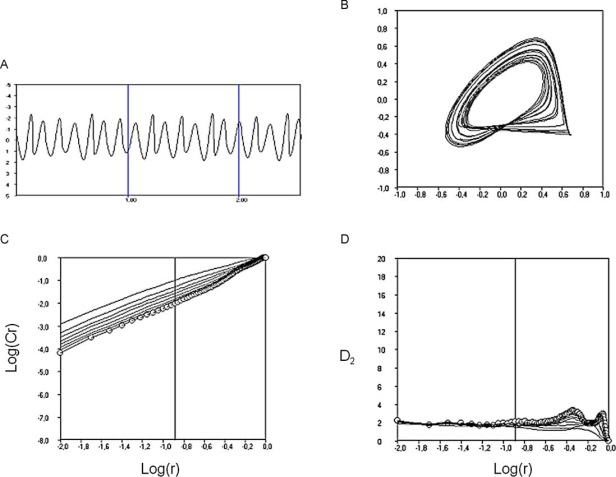
\includegraphics[width=0.8\textwidth]{Images/corrdim.png} }
  \caption{Computation of the correlation dimension \cite{stam2005}. TODO: Add description.}
\label{fig:corrdim}
\end{figure}

The world of mathematics offers numerous definitions of dimension (box-counting dimension (\ref{eq:box-counting}), Hausdorff dimension, information dimension, etc.) and similar quantities, but many of them can be regarded as variations of the following, simple and intuitive analogy:
\begin{align*}[\cite{theiler1990estimating}]
  \text{bulk} \approx \text{size}^{\text{dimension}} \implies \text{dimension} = \lim_{\text{size} \rightarrow 0} \frac{\log \text{bulk}}{\log \text{size}}.
\end{align*}
In other words, dimension can be loosely defined as scaling of ``bulk'' (corresponds to mathematical concept of measure) as a function of its linear ``size''. Of course, dimensions of different definitions may not be equal to each other, but for our purposes, we are interested in the most computationally accessible.

Unlike Lyapunov exponents, which measure dynamical properties of the system, (correlation) dimension is a purely geometrical property of the attractor, independent of the ordering of the reconstructed vectors.\unsure{Is this true?}

In this thesis, we are interested in dimension estimation for the following reasons:
\begin{enumerate}
  \item Even a system with high number of degrees of freedom, such as a brain, may actually evolve in a much lower-dimensional subspace. The number of active degrees of freedom may provide a measure of complexity of the observed system. This information is available in the attractor of the system and it can be shown that this property is preserved by state space reconstruction. \cite{andreas2000}
  \item It can help distinguish stochastic and deterministic processes, since stochastic processes, after sufficient passage of time, use all available state space dimensions.
\end{enumerate}
Of course, although these expectations can be justified theoretically, the numerical reality may be different.

Most definitions of dimension are based on first covering the studied object in the state space with the smallest possible balls (using a given metric). Correlation dimension is a special case of generalized box-counting dimension (which is a generalization of box-counting dimension already introduced in Definition \ref{def:box-counting}), defined as
\begin{align*}
  d_{\kappa}(A) = \lim_{r \rightarrow 0} \frac{1}{\kappa} \frac{ \log \int_M (\mu(B_r(\mathbf{x})))^{\kappa} \diff \mu( \mathbf{x})}{ \log r},
\end{align*}
where the integration is over the whole state space $M$ and $\mu$ is measure concentrated on $A$.
If we define $\mu$ as
\begin{align} \label{eq:measure}
  \mu(\mathbf{x}) \coloneqq \int_M \Phi (r - \norm{\mathbf{x} -\mathbf{y}}) \diff \mu (\mathbf{y})
\end{align}

The we can write the, ``bulk'' of $A$, so called generalized correlation integral as
\begin{align*}
C(\kappa, r) = (\int_M \left( \mu(B_r(\mathbf{x})))^{\kappa} \right)^{\frac{1}{\kappa}} = \left[ \int_M \left(\int_M \Phi (r - \norm{\mathbf{x} -\mathbf{y}}) \diff \mu (\mathbf{y})) \right)^{\kappa} \diff \mu (\mathbf{x}) \right]^{\frac{1}{\kappa}} 
\end{align*}
It can indeed be shown that $C(\kappa, r) \propto r^d_{\kappa}$.

In the continuous case, correlation dimension than takes to form
\begin{align*}
  d_2(A) = \lim_{r \rightarrow 0} \frac{\log C(r,2)}{\log r}.
\end{align*}

\subsubsection{Grassberger-Procaccia algorithm}
There are essentially three ways of computing correlation dimension: box-counting algorithms, pairwise distance algorithms, and nearest neighbors algorithms. Grassberger-Procaccia algorithm, which we use to compute correlation dimension, is a variant of a pairwise distance algorithm.

This class of algorithms, used in discrete cases with limited amount of data, estimates the measure of a box centered on point $\mathbf{x}_i$ in the reconstructed space as
\begin{align*}
  \mu_i = \frac{1}{N_{(m,\tau)}}
\end{align*}
and zero everywhere else.

Thus, in the discrete case, the correlation sum $C(r)$ can be computed as 
\begin{align} \label{eq:corrsum}
  C(r) \coloneqq C(r,2) = \frac{2}{N_{(m,\tau)}(N_{(m,\tau)}-1)} \sum_{i<j} \Phi(r-\norm{\textbf{x}_i - \textbf{x}_j}).
\end{align}
which corresponds to the fraction of points in the phase space whose distance is smaller than $r$. Under certain reasonable conditions, correlation sum is an unbiased estimator of the correlation integral. \cite{ScholarpediaGpa}

Typical behavior of the correlation sum is shown in Figure \ref{fig:exp-cr}. We can see that the curves are forced to meet at the same point for all $m$ - for high enough $r$, all points are counted and $C(r)=1$ (or $C(r) = \binom{N_{(m,\tau)}}{2}$ not normalized). As the lines shift to the right with increasing $m$ and stay parallel in the proper scaling region, the slope near that point necessarily increases with $m$. For high enough $m$, the scaling region disappears. Moreover, the values of $C(r)$ are inaccurate for small $r$ due to noise and for small $C(r)$ due to statistical fluctuations (corresponding to horizontal lines). Thus, there is only a limited interval of $r$ and limited set of embedding dimensions $m$ for which an accurate estimation of $d_2$ can be made. \cite{andreas2000}

\begin{figure} 
\centering
\noindent\makebox[\textwidth]{%
  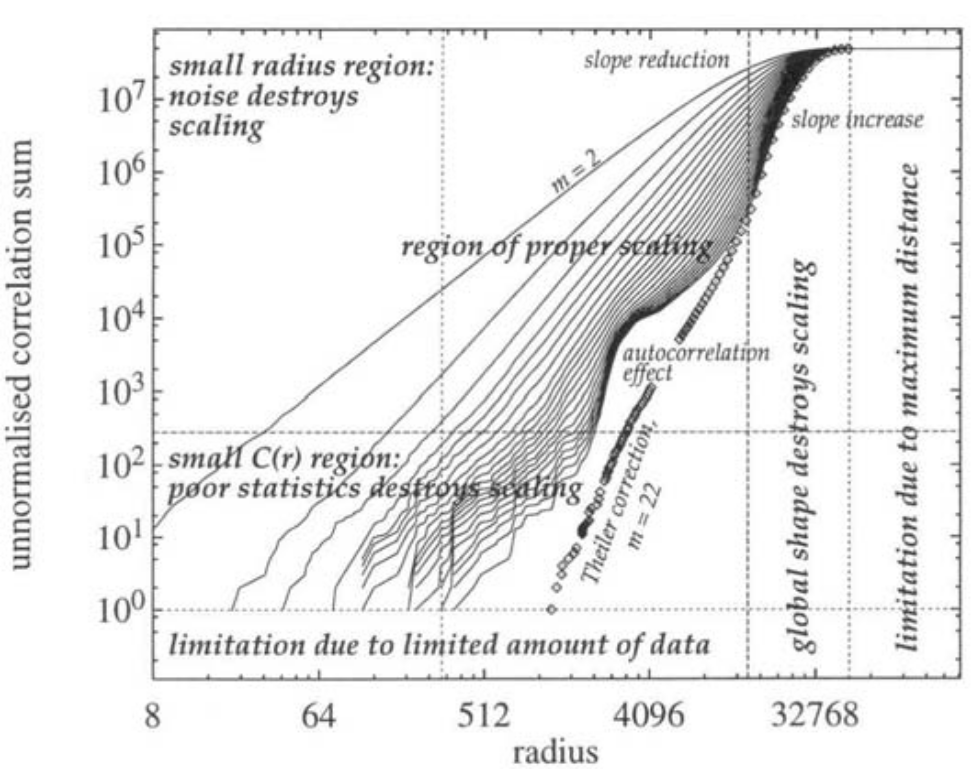
\includegraphics[width=0.6\textwidth]{Images/typ-cr.png} }
  \caption{Log-log plot of typical behavior of $C(r)$.}
\label{fig:exp-cr}
\end{figure}

In our experiments, we used \emph{local slopes approach} to estimating the correlation dimension, which is based on the idea of assigning a dimension estimate to each value of $r$ by defining
\begin{align*}
  d_2(r) = \frac{\partial \log C(r)}{\partial \log r}.
\end{align*}
In our implementation, we perform a least squares fit of values $(\log r, \log C(r))$ for a window of 6 neigboring points for each sampled $r$. Expected behavior of the resulting function in a favorable case can be seen in Figure \ref{fig:exp-localcr}.

\begin{figure} 
\centering
\noindent\makebox[\textwidth]{%
  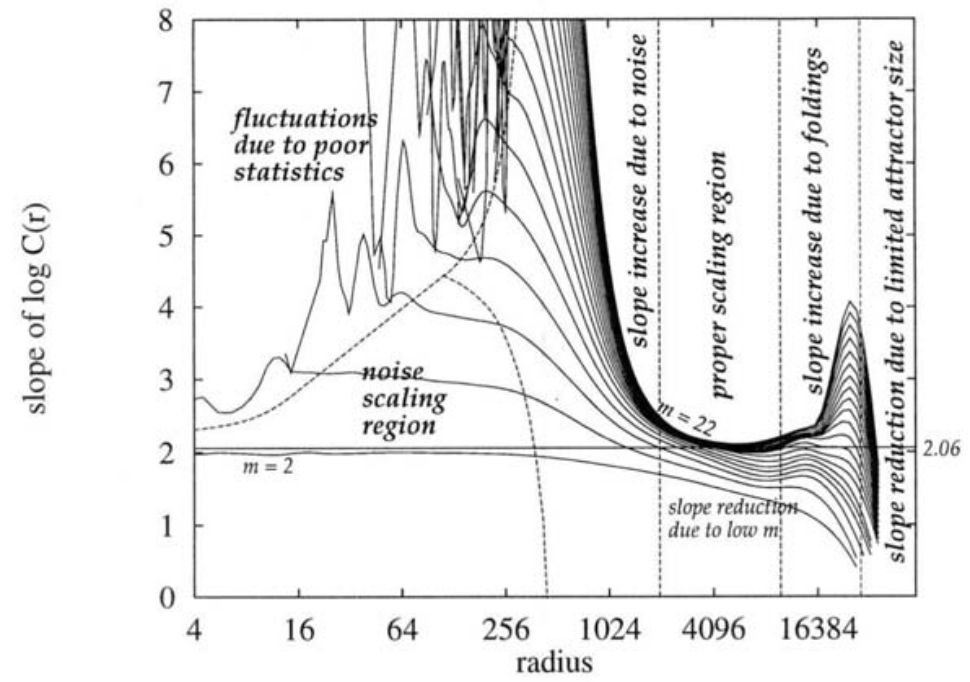
\includegraphics[width=0.6\textwidth]{Images/typ-localcr.png} }
  \caption{Log plot of a typical local dimension estimates in favorable case.}
\label{fig:exp-localcr}
\end{figure}

\subsubsection{Dataset size requirements} \label{sec:req-corr}
There are multiple estimations of the minimum dataset size. Most of them are based on an attempt to avoid so called \emph{edge effect}. It can be shown that the correlation dimension for a hypercube in $m$-dimensions of unit edge length the local correlation dimension is
\begin{align*}
  d_2^{(m)}(r) = m - \frac{mr}{2-r} \approx m(1 - \frac{r}{2}).
\end{align*}
For large enough $r$, $d_2^{(m)}(r)$ converges to zero. This result, which can be generlized to any finite object, is a consequence of the discontinuity of the measure (\ref{eq:measure}) at the boundaries of the hypercube. Theiler, assuming evalution of the local correlation dimension for radius where each point has on average one neighbor (such that $C(r) = 1/N_{(m, \tau)}$), derived an estimate for the minimum data set size as
\begin{align*}
  N_{(m, \tau)} = \frac{1}{(4\rho)^m},
\end{align*}
where $\rho$ is the maximum error. This implies an exponential increase of minimum required dataset size with embedded dimension. For example, $N_{(m, \tau)} = 5^m$ for $\rho = 5\%$. \cite{andreas2000}

\section{Surrogate data testing}
It has been shown that, for example, fitered noise can mimic low-dimensional chaotic attractors when examined by Grassberger-Procaccia algorithm described above. \cite{rapp1993filtered} Hence, interpretation of results obtained by non-linear analysis require judgement. For example. obtaining finite-dimensional estimates for $d_2$ is not evidence of non-linearity, but may indicate lack of data, measurement error, on numerical inaccuracies. The result of these algorithms does not include any error estimate, and sometimes even non-linearity of the underlying process is uncertain. So, one may ask: would we obtain the same estimate for data with the same (non-measured) linear properties as the original, but differs in the (measured) non-linear property? In the following, we will describe a method for answering this question. \info{We may also want to know whether the process is determinsitic or not. There are tests for that, but we are not using them in this thesis.}

To this end, we construct a Monte Carlo hypothesis test of non-linearity. We choose a null hypothesis of a model for the process creating obtained data which denies the property we assume to measure. For each time series, we create so called \emph{surrogate data} which deliberately capture only properties consistent with chosen null hypothesis, and compute the estimates using the same method as for the original data. If the result for the original time series is significantly different from the surrogate estimates, we reject the the null hypothesis. In the opposite case, we fail reject the null hypothesis. A schematic depiction of the process can be seen in Figure \ref{fig:surr-schema}.

\begin{figure} 
\centering
\noindent\makebox[\textwidth]{%
  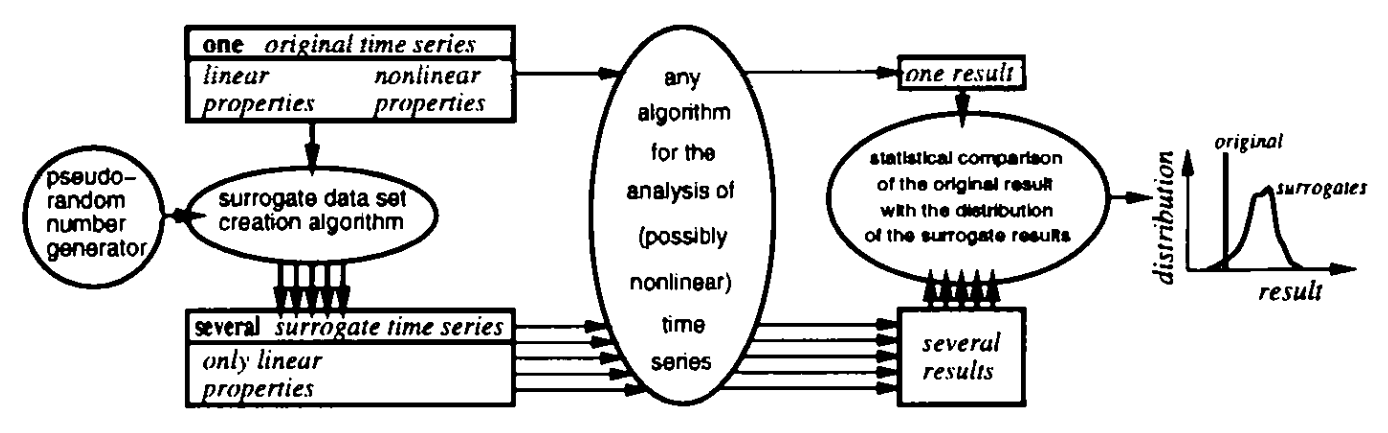
\includegraphics[width=0.8\textwidth]{Images/surr_schema.png} }
  \caption{ \cite{andreas2000} }
\label{fig:surr-schema}
\end{figure}

Here, we use two sided test, and measure of significance is defined as
\begin{align*}
  \mathcal{S} \equiv \frac{| Q_{\text{orig}} - \mu_{\text{surr}} |}{\sigma_{\text{surr}}},
\end{align*}
where $Q_{\text{orig}}$ is the statistic computed for the original time series, and $\mu_{\text{surr}}$, $\sigma_{\text{surr}}$ are the mean and variance of the statistic computed for the surrogate time series. \cite{theiler1992testing} If we assume that distribution of the generated is Gaussian, than $\mathcal{S} \geq 2$ is required for 95 \% significance level. However, validity of this assumption is not always guaranteed. For non-Gaussian distributions, we may require larger $\mathcal{S}$, or, alternatively, use a rank based test, as follows. \cite{kantz2004}

Using rank-based test, we want to test if $Q_{\text{orig}}$ is smaller or larger than the expected value of estimates produced by the null hypothesis model. If we generate $n_s$ surrogate estimates, then, we have $n_s$ estimates following the null hypothesis, each having a probability $2/n_s$ of being the smallest or largest. A false rejection will happen if $Q_{\text{orig}}$ happens to also follow the null hypothesis and is either the smallest or the largest, which happens with probablity $1 - \alpha \coloneqq 2/(n_s+1)$, where $\alpha$ is the confidence level. Hence, for confidence level $\alpha = 95 \%$, the number of surrogates should be $n_s = 38$. \cite{andreas2000}

\subsubsection{Generating improved amplitude adjusted surrogates}
For our purposes, since we assume that the data are produced by a non-linear process, a reasonable null hypothesis may be that the data are produced by a Gaussian linear stochastic process $\mathrm{AR}(p)$
\begin{align} \label{eq:lin-stoch-proc}
  x_{t+1} = \mu + \sum_{j=0}^{p-1} a_j x_{t-j} + \sigma e_t,
\end{align}
with unknown parameters $a_j, e_t, \mu, \sigma \in \RR$. \cite{theiler1992testing}

If the computed non-linear statistic depends on the free parameters in $\mathrm{AR}(p)$ (\ref{eq:lin-stoch-proc}) (which is not true, e.g. for $d_2$), then one may try to estimate these parameters from the original time series. Alternatively (and this is the approach we use in our analysis), one may exploit the fact that $\mathrm{AR}(p)$ can be also perfectly described by its power spectrum. \cite{theiler1992testing}\footnote{This is due to Wiener-Khinchin theorem, which states, roughly, that spectral decomposition of autocorrelation of a stationary process is the power spectrum of the process.} Hence, to obtain a surrogate, one may simply perform a Fourier transform of the original time series, randomize phases, and apply inverse Fourier transform. This way, the amplitudes (composing the power spectrum) are preserved. This procedure has been named \emph{Fourier transform phase randomization} (FTPR).

However, there is a drawback of FTPR. It has been shown that if the amplitudes of $\mathrm{AR}(p)$ are not Gaussian (as in (\ref{eq:lin-stoch-proc})), e.g. non-linear,\unsure{e.g. or i.e. here?} then the surrogates created using this method show non-linear behavior. \cite{kantz2004} Rarely do the amplitudes of an experimental process follow a Gaussian distribution. Hence, we change our model to correspond a non-linear, time independent filter applied to the output of $\mathrm{AR}(p)$. Surrogate creation algorithm for this model was described by Theiler in \cite{theiler1992testing}: rescale the values of the original time series so that they are Gaussian, apply FTPR described above, rescale the values back to follow the same distribution of the original time series. This surrogate creation method is called \emph{amplitude-adjusted Fourier transform} (AAFT), and has been successfully applied to EEG signal. \cite{theiler1994evidence}

Even this method is not without its drawbacks: due to the final reordering, the original power spectrum is slightly distorted in the surrogate. In \cite{theiler1994evidence}, it was proposed how to mitigate this effect. The amplitudes of Fourier transform of AAFT surrogates are replaced by the amplitudes of the original time series. The power spectrum is now correct, but the distribution is wrong. So, the original time series is reordered to according to ranks of values in this surrogate. This results in precisely the desired distribution of values, but again, slightly deviant power spectrum. These steps are then iterated and, experimentally, they results seem to converge. Hence, the final procedure, called \emph{improved (iterated) amplitude-adjusted Fourier transform} (iAAFT) can be summarized as follows: \cite{andreas2000}

\add[inline]{Maybe talk about the problems, e.g. endpoint mismatch? We will need to refer to them later.}

\begin{enumerate}
  \item Compute and store the moduli of the original time series.
  \item Create an AAFT surrogate as follows:
    \subitem Create a set of random numbers with Gaussian distribution.
    \subitem Rank order the original time series, and reorder the random numbers created in the previous step such that they achieve the same ordering as the original time series.
    \subitem Randomize the phases Fourier transform of the time series obtained in previous step and apply inverse Fourier transform.
    \subitem Find the rank ordering of the time series obtained in the previous step, and reorder the original time series so that it assumes the same rank ordering.
  \item Replace the moduli of these surrogates by those of the original time series and apply inverse Fourier transform.
  \item Find the rank ordering of the time series obtained in the previous step, and reorder the original time series so that is assumes the same rank ordering.
  \item Apply step 3. to time series obtained in the previous step, or stop if stopping criterion is reached.
\end{enumerate}

\section{Applications in disease diagnosis}\label{sec:applications}
\add[inline]{This section is probably not sufficiently exhaustive.}
Although non-linear dynamical analysis of EEG signal has been successfully applied to many psychological and psychiatric conditions, such as insomnia, schizophrenia, epilepsy, dementia, Alzheimer's disease, the number of studies applying methods of non-linear time series analysis for clinical depression diagnosis is relatively limited. \cite{rodriguez2015}

It has been found that the EEG dynamics of depressed patients exhibit more predictability than those of non-depressed ones, with this indicator receding after treatment. \cite{nandrino1994} \cite{pezard1996}

Another study analyzed sleep EEGs of depressed and control subjects, and found significantly decreased values of Lyapunov exponents in a sleep stage IV in depressed relative to control. \cite{roschke1995}

In 2012, Ahmadlou et al. decomposed 5 EEG channels recorded from frontal lobes of healthy and depressed patients using wavelet filter banks, measured their complexity using Higuchi's fractal dimension, subsequently used ANOVA to discover the most meaningful differences between the groups, and trained a probabilistic neural network classifier, achieving 91.3\% classification accuracy on limited amount of data. This research suggested potential of frontal lobe signal assymetry as a measure for depression. \cite{ahmadlou2012}

In the same year, Hosseinifard et al. extracted Higuchi's correlation dimension, Lyapunov exponents and Higuchi's fractal dimension from 4 EEG channels of 90 patients split evenly between depressed and non-depressed subjects, achieving 90\% accuracy using a logistic regression classifier. \cite{hosseinifard2013}

In 2013, Bachmann et al. compared two non-linear analysis methods, spectral assymetry index (SASI) and Higuchi's fractal dimension (HFD), for depression diagnosis, on 34 subjects split evenly between depressed and control group. SASI achieved true detection rate in 88\% in depressives and 82\% in the controls, while HFD provided true detection rate of 94\% in the depressives and 76\% in the controls. \cite{bachmann2013}

Sleep disorder diagnosis may also relevant to this work for the very close connection of depression with disturbed sleep and insomnia \cite{nutt2008}. The first study emplying techniques of non-linear analysis on human EEG was published in 1985 and dealt with sleep recordings. \cite{babloyantz1985} This early success sparked intensive research focus on applying non-linear analysis to sleep data, thus generating relatively large amount of results. 

Many studies focused of extracting Lyapunov exponents of EEGs measured during various sleep stages. The general pattern that emerged was that deep sleep stages exhibit lower complexity evidenced by lower dimensionality lower values of the largest Lyapunov exponent \cite{stam2005}.

\chapter{Non-linear analysis approach}

\section{Dataset}
The EEG recordings were performed by and obtained from the Czech National Institute of Mental Health. The dataset comprises total of 133 subjects, 104 women and 29 men, ranging in age from 30 to 65 (47.7 $\pm$ 9.58). Geriatric Depession Scale questionnaire assessed by a trained psychologist was used to measure depression severity. This psychometric measurement results in a depression score ranging from 0 (normal) to 40 (severe depression). 

The experiment lasted 4 weeks. At the beginning of week 1, each subject's depression score was measured, their EEG signal was recorded, and, based on the measurement and patient's history, prescription of up to 4 drugs was made. After 4 weeks, depression score was remeasured and EEG signal recorded again.

During the EEG recording, 19 electrodes were placed on the scalp in accordance with the Internation 10-20 system (FP1, FP2, F3, F4, C3, C4, P3, P4, O1, O2, F7, F8, T3, T4, T5, T6, Fz, Cz, Pz), see Figure \ref{fig:electrodes} for reference. EEG signals of 99 subjects were recorded at sampling frequency $f_s$ of 250 Hz, while 1000 Hz was used for the remaining 34 patients. The patients were not told to close their eyes for the duration of the recording, resulting in unwanted artifacts in the signal. Some of the artifacts were removed manually by the researchers by omitting those parts from the recording, and concatenating the remaining parts. Durations of the resulting measurements range from 23.5 s to 170 s (75.6 $\pm$ 20 s) for $f_s = 250$ Hz , and from 48.8 s to 140.4 s (79.5 $\pm$ 18.4 s) for $f_s = 1000$ Hz.

A typical recoding can be seen on Figure \ref{fig:data}.

\begin{figure} 
\centering
\noindent\makebox[\textwidth]{%
  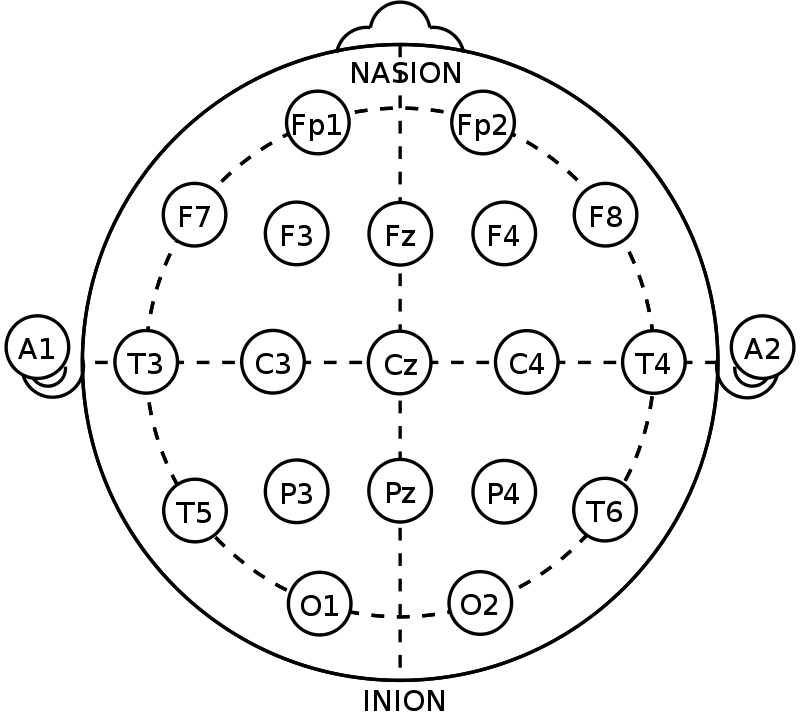
\includegraphics[width=0.5\textwidth]{Images/electrodes.png} }
  \caption{}
\label{fig:electrodes}
\end{figure}

\begin{figure} 
\centering
\noindent\makebox[\textwidth]{%
  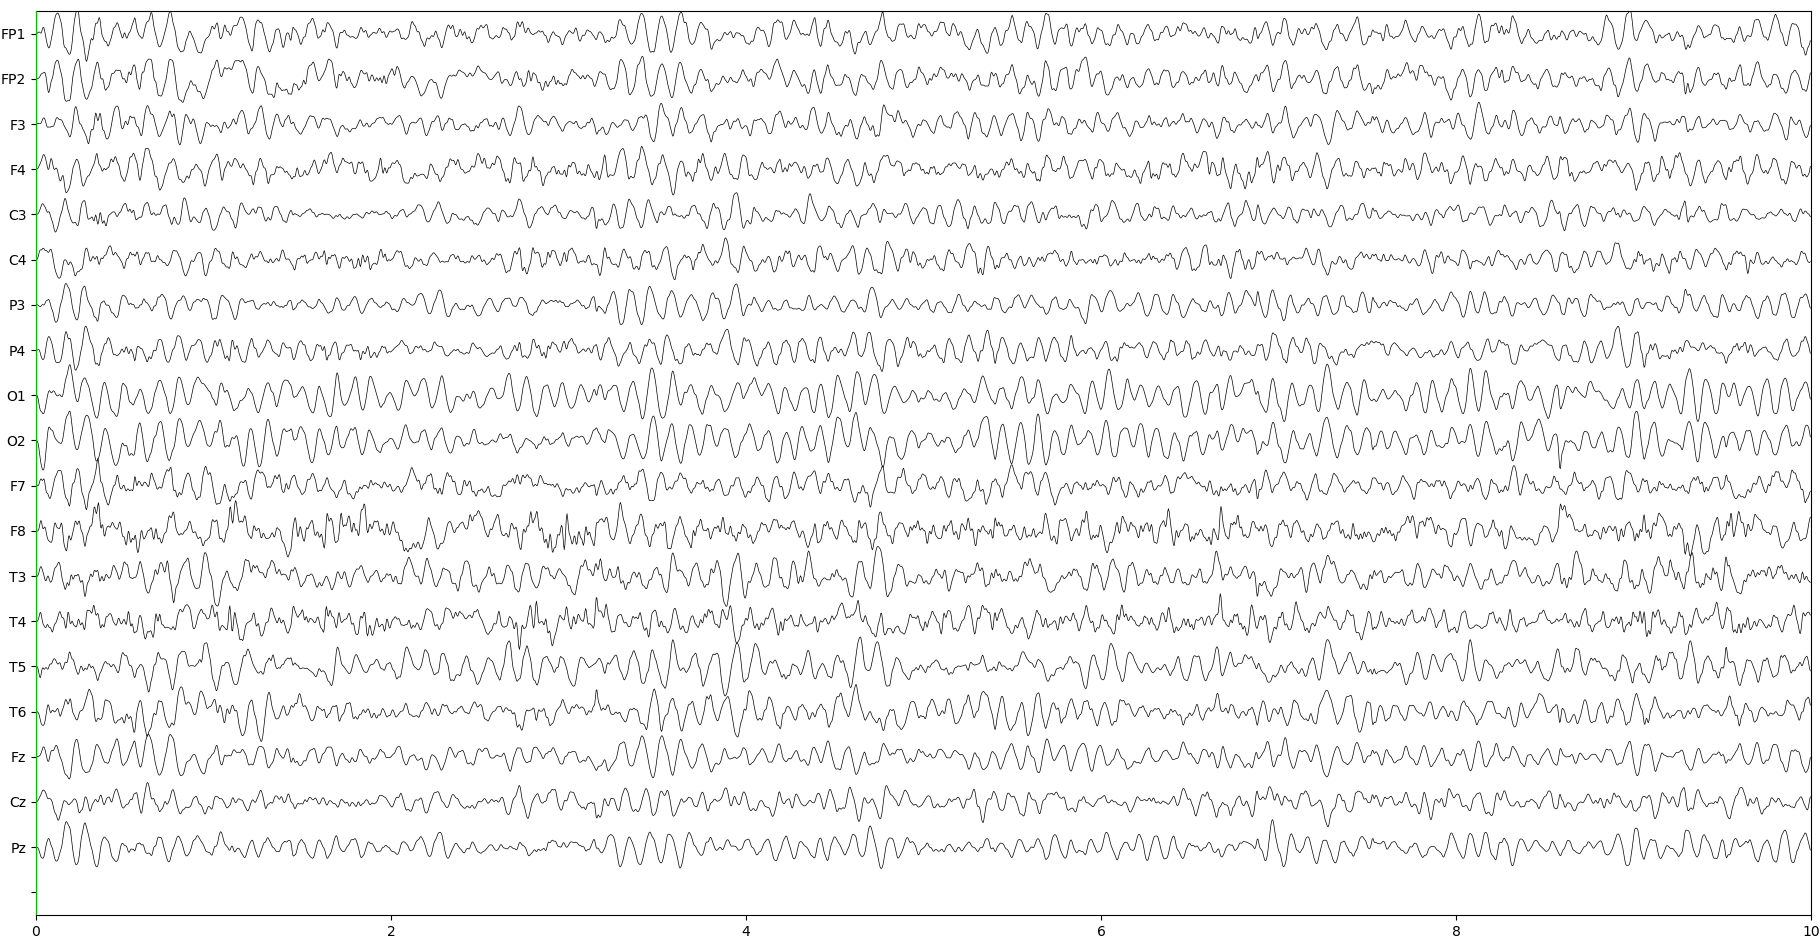
\includegraphics[width=1.0\textwidth]{Images/data.png} }
  \caption{}
\label{fig:data}
\end{figure}

\section{Preprocessing}
Recordings of $f_s = 1000$ Hz were downsampled (decimated) by factor $4$ to $250$ Hz using the Fourier method (also known as trigonometric interpolation), i.e. by performing discrete Fourier transform on the original series, dividing it into $2*1000/250=8$ intervals, removing all but the first and the last intervals (thus removing the highest positive and negative frequencies, corresponding to low-pass filtering), and performing inverse discrete Fourier transform. This procedure assumes that the signal is periodic, and may have some influence on the obtained results. However, it was observed that this effect is almost negligible, even for considerably higher decimation factors. \cite{diab2013effect}

In further analysis, unless otherwise specified, recordings were shortened to a fixed length. To balance the data requirements (see Sections \ref{sec:req-lyap} and \ref{sec:req-corr}), decrease in dataset size due to removal of too short recordings, and stationarity (see Section \ref{sec:stationarity}), the threshold was selected to be 60 s (15 000 datapoints per time series), resulting in exclusion of 26 recordings from the total of 266.

In some studies, band-pass filtering was used to remove frequencies which are physiologically impossible to produce by neural oscillations (e.g. high-pass filtering with 0.5 Hz threshold or lowpass filtering with 70 Hz threshold). \cite{hosseinifard2013} Sometimes, it is suggested to notch filter at power line frequencies (40 Hz or 50 Hz). However, some authors suggest that linear filtering may adversely affect the results of non-linear analysis. \cite{andreas2000} Others, on the other hand, observed that simple linear filtering does not influence the reconstruction of embedding space considerably. \cite{Rohrbacker2009} If quality of the data is sufficient, filtering is not necessary. \cite{Jas2017} By visual inspection, we found our data to be of sufficient quality and therefore decided to not risk influencing the results by filtering. \info{In fact, we tried both, but for filtered the results looked slightly more uniform.}

\section{Stationarity}
Stationarity was evaluated on multiple time scales using the stationarity test described in Section \ref{sec:stationarity}. For results, see Table \ref{tab:stat}.

\begin{table}[tbp] 
\centering
\begin{tabular}{|c|c|c|}
\hline
\textbf{Duration\textbackslash Av. p-value} & \textbf{Original} & \textbf{Surrogate} \\ \hline
10 s                                         &                   &                    \\ \hline
30 s                                         &                   &                    \\ \hline
60 s                                         &                   &                    \\ \hline
\end{tabular}
\caption{Results of stationarity tests.}
\label{tab:stat}
\end{table}

\section{State space reconstruction}
\subsection{Surrogate data}
\add[inline]{Describe process of generating surrogate data.} See Figure \ref{fig:ts}.

\begin{figure} 
\centering
\noindent\makebox[\textwidth]{%
  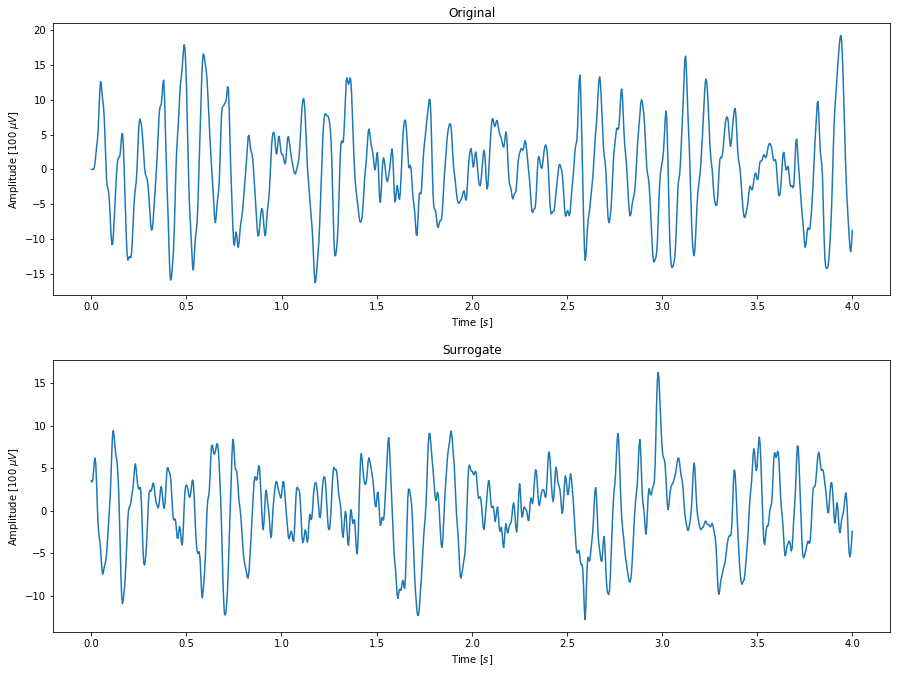
\includegraphics[width=1.0\textwidth]{Images/ts.png} }
  \caption{The first 4 $s$ of a time series and its surrogate.}
\label{fig:ts}
\end{figure}

\subsection{Time delay}
In order to estimate the time delay, we used the following techniques:
\begin{enumerate}
  \item Reconstruction plots
  \item Autocorrelation $A(\tau)$ (see Section \ref{sec:acorr})
  \item Delayed mutual information $\mathcal{I}(\tau)$ (see Section \ref{sec:dmi})
  \item Average displacement from diagonal (ADFD) (see Section )
  \item PCA reconstructions comparison (see Section )
  \item Integral local deformation (ILD) (see Section )
\end{enumerate}

In this section, we will analyze the results of these techniques for time series obtained from FP1 electrode of patient 75, second session, shown in Figure \ref{fig:ts}. The time series was clipped to 60 s (15000 data points). In the following sections \change{Add concrete references.}, we will explain how these techniques were used to obtain estimates of individual non-linear measures.

Figure \ref{fig:recon} shows reconstructed trajectories for the first 4 s (1000 data points) of the recording, for varying time delay $\tau$. As expected, the reconstructed attractors for small delays cluster along the main diagonal, expand, and then become increasingly chaotic with larger $\tau$. However, it is impossible to judge objectively on the degree of folding in the attractor from these plots (even for shorter time series), which highlights the importance of qualitative measures for EEG signals.

Typical plots of autocorrelation and delayed mutual information can be seen on Figure \ref{fig:dmi-acorr}. First local minima of DMI and first $\tau$ for which $A(\tau) \leq 1/e$ are marked by yellow dots. For this channel, these are $\tau_{\mathrm{DMI}} = 7$ and $\tau_{A} = 6$. These values were computed for all channels of this recording, and their distribution for both DMI and autocorrelation can be seen in Figure \ref{fig:dmi-acorr-hist}. For this patient, autocorrelation shows less variance and lower suggested time delays. This behavior was observed across patients. \add{I should provide mean $\tau$ reported by $A(\tau)$ and DMI for all recordings.}

Figure \ref{fig:pca-svd} shows singular values of the PCA reconstruction as functions of $\tau$. The two prominent singular values correspond to the main axes \unsure{Is this correct?} of the attractor. We can see several collapses: smaller ones at $\tau = 5$ and $\tau=7$, and larger one at $\tau=14$, corresponding to the sharp peak of ILD on Figure \ref{fig:ild}. For $\tau=3$, the three largest singular values show convergence - however, the small singular values suggests that the attractor has not fully unfolded in their corresponding directions. \unsure{Not sure if this wording is precise and understandable.} Overall, this behavior suggests $\tau_{\mathrm{svd}} = 6$ as optimal. Note that results of this technique are difficult to evaluate by an automatic procedure.

The results obtained by ADFD can be seen in Figure \ref{fig:adfd}. The average displacement tends to increase with $m$, is not monotonically increasing on its domain, and saturates for relavely small values of $\tau$ - thus, the estimated time delays are (consistently)\change{We need to smartly separate general observations with this analysis.} lower than those obtained by other techniques. Moreover, this technique requires prior selection of $m$. However, the algorithms for selection of $m$, require estimation $\tau$, making this technique impractical.

The result of ILD, the most powerful algorithm for estimation of the embedding parameters we used, can be seen on Figure \ref{fig:ild}. There is a clear minimum at $\tau_{\mathrm{ILD}}=4$, and the ILD curves become very similar for approximately all $m \geq 10$, except near the minimum, where they converge slower. Almost identical behavior was observed across all channels in this recording. \add{There are interesting patterns in these plots across patients and channels.} This algorithm is computationally expensive (it takes around an hour to generate a single plot), and so is impractical for large datasets.

As explained in Section \ref{sec:delay}, these techniques should be used only as inspection tools, not as reliable guides for selection of $\tau$. The ultimate goal of the reconstruction is to obtain as accurate values of the non-linear parameters as possible, and thus selection of the optimal embedding parameters may differ for each of them.\unsure{Find some studies doing this also. Is there a way to justify this theoretically?} Thus, for example, in order to select the proper embedding parameters for computation of the largest Lyapunov exponent, we inspected the scaling regions for multiple values of $m$, $\tau$, Theiler window\add{Add description of Theiler window to \ref{sec:rosenstein}}, and other parameters, and picked those with the longest scaling regions (since the length of the scaling regions is proportional to the certainty of the estimate \cite{kennel1992determining}).

Table \ref{tab:delay-est} shows an overview of estimated values of $\tau$. Autocorrelation, DMI, and singular values analysis report lower values than ADFD and ILD. However, Rosenstein notes that the best estimates of largest Lyapunov exponents were obtain for the autocorrelation threshold of $1-1/e$. For this threshold, the autocorrelation suggests $\tau_A = \tau_{ILD} = 4$ as optimal (and the distributions shift accordingly), thus in agreement wil ILD.  

In the Section \ref{sec:lle-exp}, we will show the effects of increasing $\tau$ on the average divergence.

\begin{table}[tbp]
\centering
\begin{tabular}{|c|c|}
\hline
\textbf{}                  & \textbf{Optimal time delay estimate} \\ \hline
Reconstruction plot        & -                                    \\ \hline
Autocorrelation            & 6, 4                                 \\ \hline
Delayed mutual information & 7                                    \\ \hline
Singular values analysis   & 6                                    \\ \hline
Average displacement       & 2, 3                                 \\ \hline
Integral local deformation & 4                                    \\ \hline
\end{tabular}
\caption{Optimal time delay estimates of individual techniques for patient 75, second session.}
\label{tab:delay-est}
\end{table}


\add[inline]{Should I implement some better methods? MI and acorr are not practical for EEG and other high dimensional systems.}

\begin{figure} 
\centering
\noindent\makebox[\textwidth]{%
  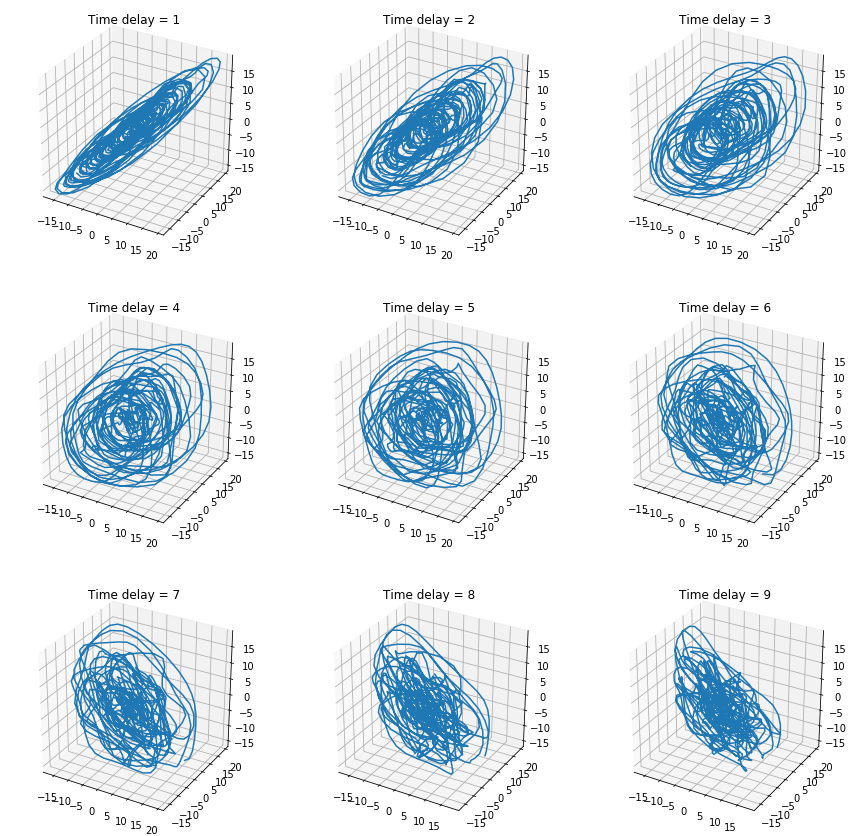
\includegraphics[width=1.0\textwidth]{Images/recon.png} }
  \caption{3D time delay reconstructions for various values of $\tau$.}
\label{fig:recon}
\end{figure}

\begin{figure} 
\centering
\noindent\makebox[\textwidth]{%
  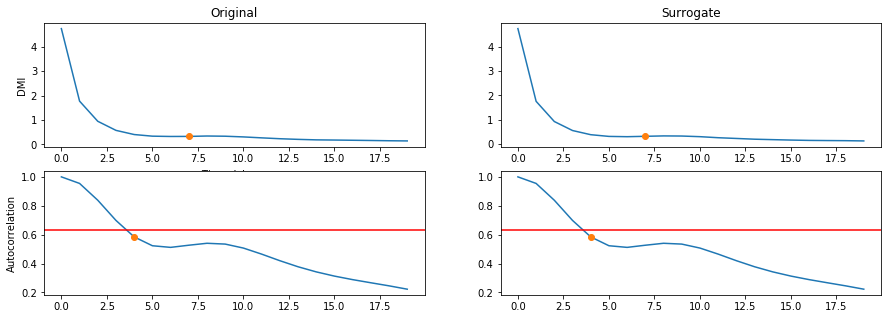
\includegraphics[width=1.0\textwidth]{Images/dmi_acorr.png} }
  \caption{Delayed mutual information and autocorrelation as functions of $\tau$. The red line shows threshold values $1-1/e$ and $1/e$ respectively. The plots of surrogate data are equivalent.}
\label{fig:dmi-acorr}
\end{figure}

\begin{figure} 
\centering
\noindent\makebox[\textwidth]{%
  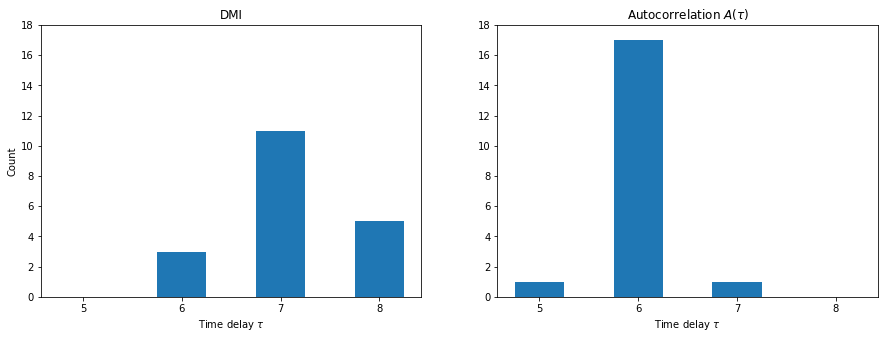
\includegraphics[width=1.0\textwidth]{Images/dmi_acorr_hist.png} }
  \caption{Distributions of time delays computed using delayed mutual information and autocorrelation for threshold $1/e$.}
\label{fig:dmi-acorr-hist}
\end{figure}

\begin{figure} 
\centering
\noindent\makebox[\textwidth]{%
  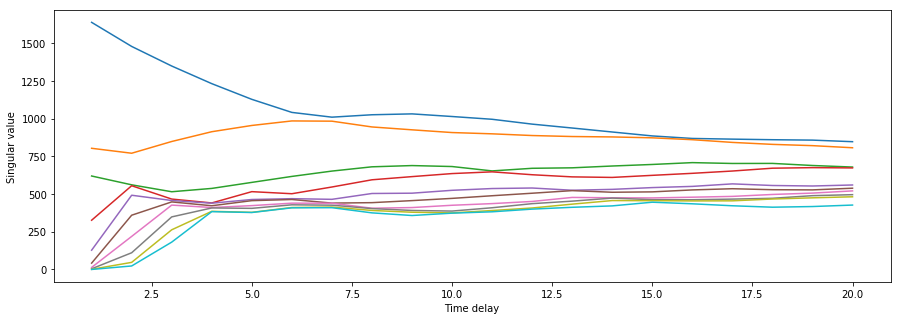
\includegraphics[width=1.0\textwidth]{Images/pca_svd.png} }
  \caption{Plot of singular values as functions of $\tau$ for $m=10$.}
\label{fig:pca-svd}
\end{figure}

\begin{figure} 
\centering
\noindent\makebox[\textwidth]{%
  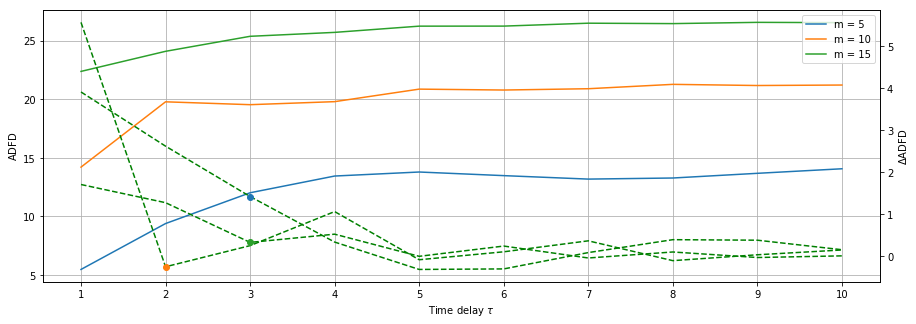
\includegraphics[width=1.0\textwidth]{Images/adfd.png} }
  \caption{Plot of average displacement from diagonal for $m=10$.}
\label{fig:adfd}
\end{figure}

\begin{figure} 
\centering
\noindent\makebox[\textwidth]{%
  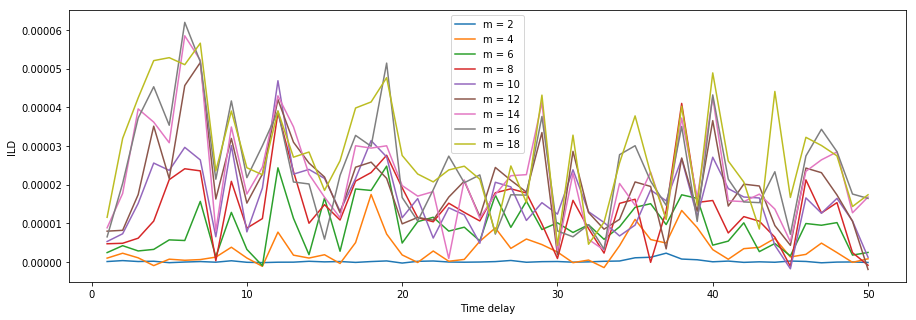
\includegraphics[width=1.0\textwidth]{Images/ild.png} }
  \caption{Plot of integral local deformation. The parameters used for this computation are $q_{\mathrm{max}} = 10$, $t_e = 3$, $N_{\mathrm{ref}} = N_v$, $k=20$ and $w_t = 10$.}
\label{fig:ild}
\end{figure}

\subsection{Embedding dimension}
For estimating the embedding dimension, we used combination of \emph{false nearest neighbors} (FNN) algorithm described in Section \ref{sec:fnn} and average false neighbors (AFN) described in Section \ref{sec:afn}. The convergence of ILD curves and saturation of correlation dimension also provides insight into optimal choice of embedding dimension.

The percentage of reported false neighbors depends strongly on the selected values of $R$ and $A$ from equations (\ref{eq:first-criterion}) and (\ref{eq:second-criterion}). This is illustrated on Figure \ref{fig:fnn-comp}, showing the percentage of false neighbors reported by the respective criteria for varying values of $A$ and $R$, and for several values of time delay $\tau$. 

The percentages reported by the criterion I are almost independent of $\tau$, whereas increasing $\tau$ tends to increase the percentage reported by criterion II. For high enough $\tau$, criterion II will report all neighbors as false. 

The apparent independence of the results of the criterion I on $\tau$ is indicates that, regardless of $\tau$, the same percentage of near neighbors changes their distance proportionally with increase in $m$. As explained in Section \ref{sec:fnn}, \add{Actually explain it there - nearest $\neq$ close, etc\dots, \cite{kennel1992determining}} this behavior that can be expected of randomly generated uniformly distributed sequence of numbers. Indeed, behavior of the criterion II is consistent with this hypothesis - it eventually increases to 100\% for all values of $A$, essentially indicating infinite dimension.

By selecting proper parameters and using both criteria cojointly, however, FNN can still be used to obtain reasonable results, consistent with estimates obtained by ILD and AFN. \add{Report average $m$ computed by ANN and FNN, $R=2.5$, $A=2.0$, $\Delta E_1 \leq 0.005$ for this patient using a histogram.}

The $E_1$ statistic of AFN usually stops increasing for approximately the same value as reported by criterion I of FNN for $R=2.5$, see Figure \ref{fig:afn-comp}. The $E_2$ statistic, tends to oscillate in small neighborhood of value $1$, which is an indecation of nondeterminism \cite{Cao1997}.

We plotted the value of correlation dimension against $m$ for various values of $\tau$ (see Figure \ref{fig:em-corrdim}) - for details about the computation, see Section \ref{sec:corrdim-exp}.\add{Add statistics of $m$ computed this way.}

\begin{figure} 
\centering
\noindent\makebox[\textwidth]{%
  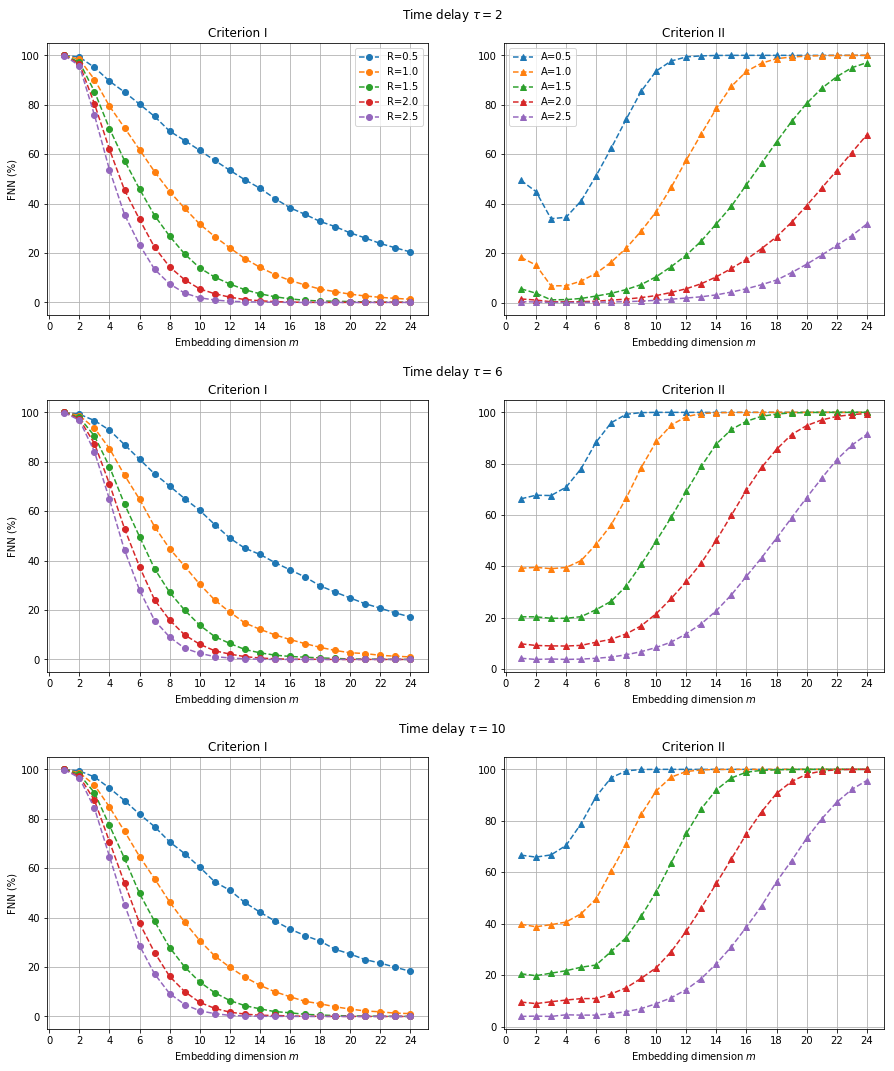
\includegraphics[width=1.0\textwidth]{Images/fnn_comp.png} }
  \caption{The effect of values of the tolerance parameters on the percentage of false neighbors reported by I. criterion (\ref{eq:first-criterion}) and II. criterion (\ref{eq:second-criterion}), Theiler window $w_t = 50$.}
\label{fig:fnn-comp}
\end{figure}

\begin{figure} 
\centering
\noindent\makebox[\textwidth]{%
  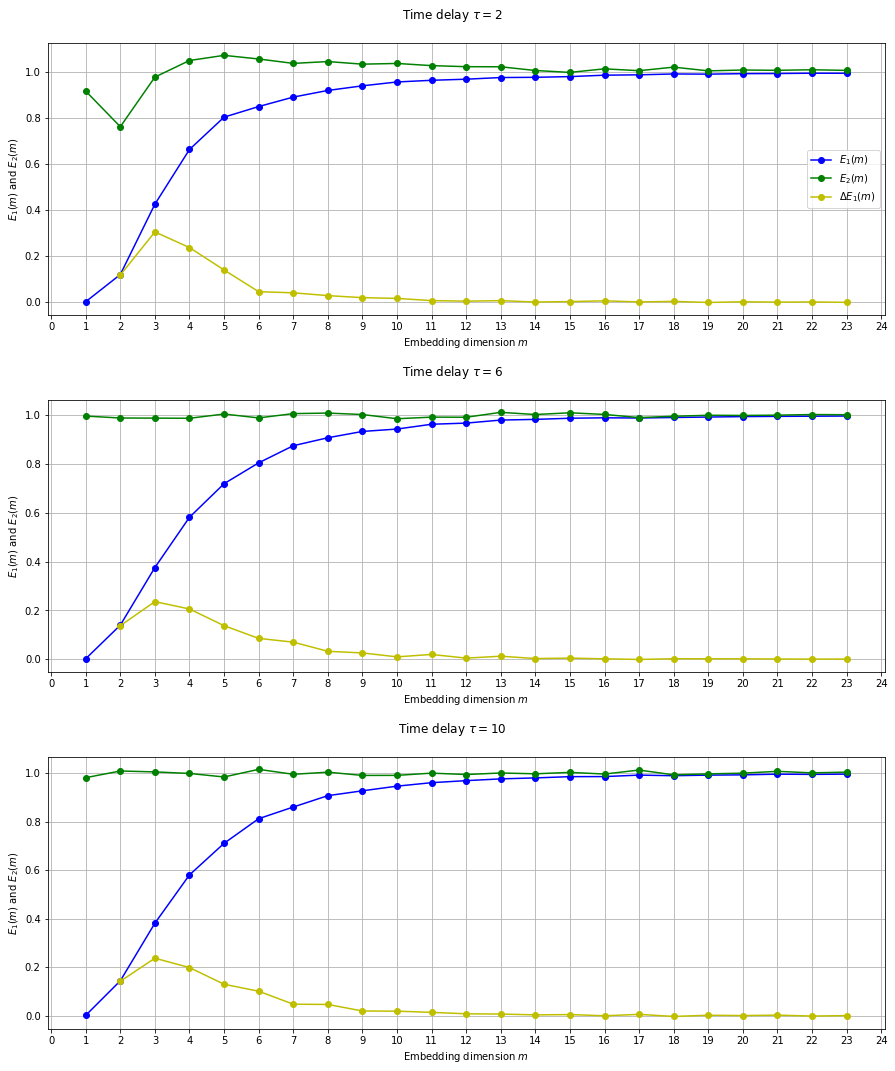
\includegraphics[width=1.0\textwidth]{Images/afn_comp.png} }
  \caption{The results of AFN for varying values of time delay $\tau$, Theiler window $w_t = 50$.  }
\label{fig:afn-comp}
\end{figure}

\section{Estimation of non-linear features}
\subsection{Largest Lyapunov exponents} \label{sec:lle-exp}
For all computations of the largest Lyapunov exponent, we used the Rosenstein's algorithm \cite{Rosenstein1993} described in Section \ref{sec:rosenstein}, with Theiler window $w_t$ length of 50 (200 ms). We found that the results were similar for values $w_t$ of 10, 50, 100 and 1000. \unsure{Why? This is unexpected.}

Figure \ref{fig:lle-comp} shows divergence plots for different values of the embedding dimension $m$ and time delay $\tau$. Let us remind the reader that longer scaling regions correspond to higher certainty of the estimate. The short scaling regions and high slopes for small embedding dimension may appear because, when the attractor is not unfolded, near neighbors are not actually close in the phase space and thus their trajectories diverge quickly. With increasing embedding dimension the scaling region clearly lengthens, but the slope also slowly approaches zero, and scaling region gradually disappears. Therefore, selecting proper embedding dimension based on divergence plots is a balancing act between those two effects. Moreover, notice that the length of the scaling region is approximately $m\tau$. \unsure{How to explain this?}

With increasing time delay $\tau$, we observe gradually damped oscillation-like behavior with period $\tau$ and amplitudes also increasing with $\tau$. Average divergence computed using Kantz' algorithm also exhibits this behavior. The explanation is as follows: let $x_1, x_2, \dots, x_N$ represent equidistantly sampled time series, and $y_i \in \RR^{m}$ an embedded point in the reconstructed orbit. Then
\begin{align*}
  y_i               &= \begin{pmatrix} x_i & x_{i+\tau} & \dots & x_{i+(m-2)\tau} & x_{i+(m-1)\tau} \end{pmatrix} \\
  y_{i+\tau}        &= \begin{pmatrix} x_{i+\tau} & x_{i+2\tau} & \dots & x_{i+(m-1)\tau} & \mu_1 \end{pmatrix} \\
                    & \dots \\
  y_{i+(m-1)\tau}   &= \begin{pmatrix} x_{i+(m-1)\tau} & \mu_1 & \dots & \mu_{m-2} & \mu_{m-1} \end{pmatrix}, \\
\end{align*}
and so if $x_i \approx x_{i+\tau}$ for enough $i$, then $y_i \approx y_{i+\tau} \approx y_{i+2\tau} \approx$, and this oscillation with period $\tau$ gradually vanishes over $m-1$ periods. \unsure{Why doesn't this happen always?}

This effect can be aleviated by choosing smaller $\tau$, but we are unaware of any way of eliminating it completely for Rosenstein's algorithm. \unsure{Are there others? Somehow introduce randomness?}\footnote{There are algorithms, such as modifications of Wolf's algorithm \cite{roschke1995nonlinear}, whose results are almost independent on $\tau$ (as is theoretically expected).} Another metric to optimize after length of the scaling region is, therefore, reduction of the degree of deformation of the scaling region by the periodic oscillations.

\info[inline]{We computed LLE for fixed $m$ and $\tau$, and then by selecting them automatically. Describe the reasoning for selecting the fixed ones, and the process of automatic selection via the method in the previous section.}

\info[inline]{Oscillation-like behavior was observed for white noise data in \cite{Rosenstein1993}, and for periodic data with period equal to the dominant period of the system in \cite{kantz2004}.}

\unsure[inline]{Can this occur due to measurement projection? Also, even if the largest Lyapunov exponent is positive, in dissipative systems (i.e. those possessing an attractor, see Section \ref{sec:attractor}) the sum of all Lyapunov exponents is negative, and thus, even on average, states will diverge in some directions. These effects can be compensated for by using proper averaging statistics \cite{kantz2004}.}

\info[inline]{We observe very similar behavior of the average divergence for the surrogate data. This, together with the observations made in previous sections, gives rise to the hypothesis of lack of chaos in the data. We tested the hypothesis of linear Gaussian process in Section \ref{sec:surrogate-analysis}.}

\info[inline]{Good thing is that Eckmann's algorithm gives similar results with very different approach. Maybe we shoud incorporate this somehow?}

To compute the LLE estimates with automatic selection of proper embedding parameters, we proceeded as follows.  First, we found the 60 s subsection of the time series with the lowest p-value of the $\chi^2$ stationarity test using moving window of length 15000 and slide 100. Selection of time delay was done using autocorrelation function with threshold $1-1/e$. The selected $\tau$ was used to compute the embedding dimension with smallest FNN percentage from embedding dimensions in range from 1 to 20, i.e. $m_1 = \argmin_{m' \in \{1,\dots,20\}} \mathrm{FNN}(m')$. The tolerance parameters wer $R=2.5$, $A=2.0$ and $w_t = 50$. Moreover, we found the first embedding dimension $m_2$ for which $E_1(m_2) - E_1(m_2-1) < 0.008$. \add{Add the average $m$'s computed this way.} The selected embedding dimension was $m = \ceil{m_1 + m_2)/2}$. The length of the scaling region $t_{\mathrm{max}} = m\tau$ and the Theiler window $t_w = 50$.

\begin{figure} 
\centering
\noindent\makebox[\textwidth]{%
  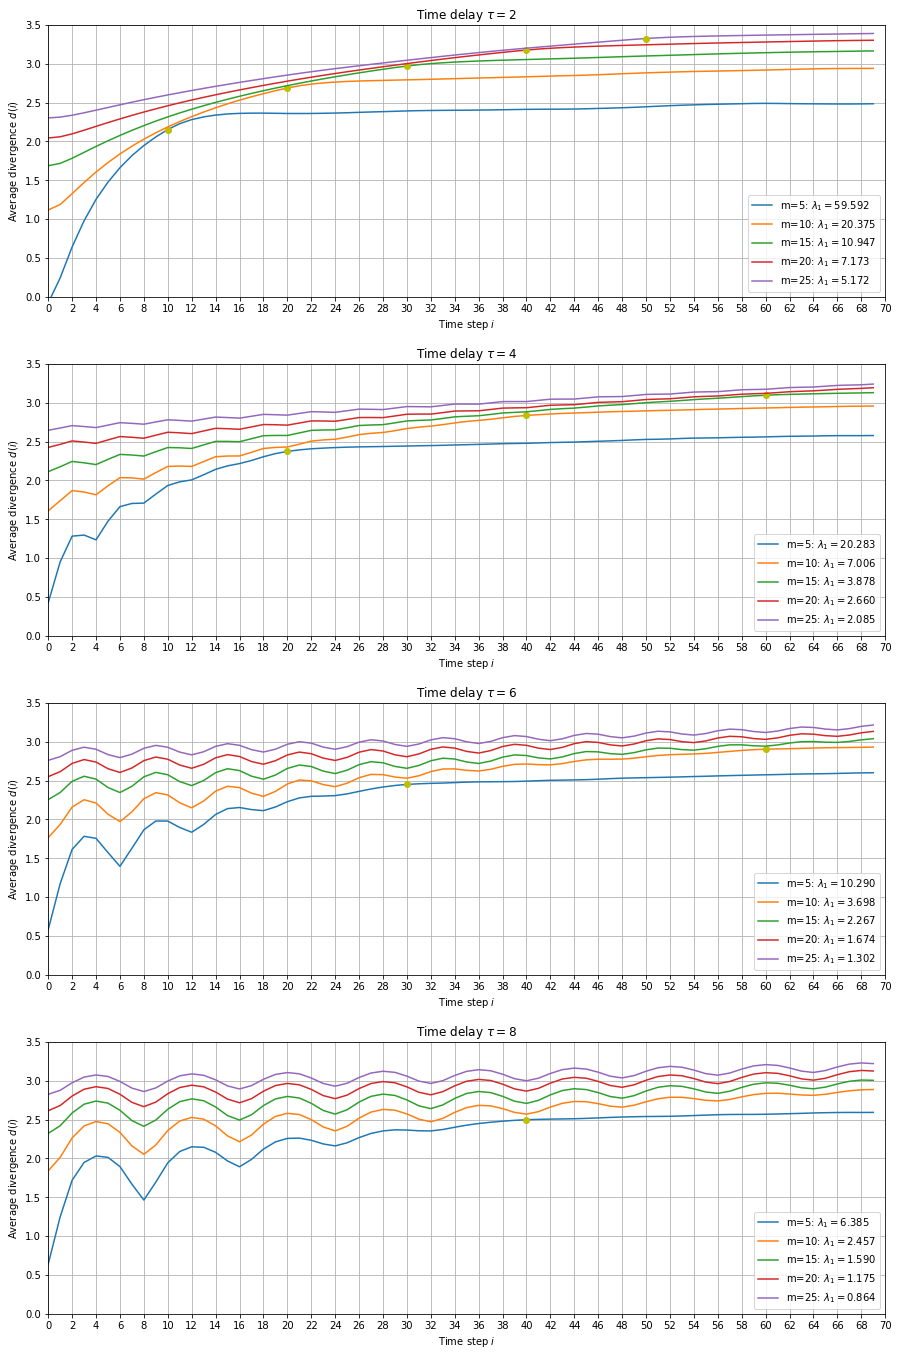
\includegraphics[width=0.9\textwidth]{Images/lle_comp.png} }
  \caption{Average divergence plots for varying values of $m$ and $\tau$.}
\label{fig:lle-comp}
\end{figure}

\subsection{Correlation dimension} \label{sec:corrdim-exp}
\info[inline]{For corr dim, we also used two ways to compute it - automatic and fixed. Explain here why have we chosen $m=10$ and $\tau=3$.}

To compute the correlation sum $C(r)$, we used classical Grassberger-Procaccia algorithm described in Section \ref{sec:corrdim} using Chebyshev metric, $w_t = 50$, for values of $r$ either in geometrical progression of 100 values from 0.05 to 10 or by an automatic procedure described further. Then, these $(r, C(r))$ pairs were used to compute local least square fits of the equation $C(r) = r^{d_2}$ inside windows of length 7 for each pair. \add{This paragraph can be much improved (wording, etc.).}

Figure \ref{fig:cr} shows log-log plots of normalized correlations sum $C(r)$ against radius $r$ for varying values of time delay $\tau$. There are clear straight lines indicating expected relationship $C(r) \propto r^{d_2}$. We can see that the lines shift to the right, increasing their slopes with $m$. The correlation sum is almost independent of time delay.

Figure \ref{fig:loc-d2} shows the log plot of local slope of of $\log C(r)$ as a function of $r$. There are no apparent scaling regions at all. Morever, by comparing with the same plot for iAAFT surrogate of the same time series (see Figure \ref{fig:loc-d2-comp}), we cannot even reject the hypothesis of a linear stochastic process. 

We decided to compute the correlation dimension as follows. First, as with computation of the Lyapunov exponent, we use a moving window of length 15000 datapoints and shift 100 to locate 60 s section of the time series with the lowest p-value for the $\chi^2$ stationarity test described in Section . \add{Add description of the test.} Then, we create embeddings for embedding dimensions in range from 2 to 30 with the optimal time lag selected according to the autocorrelation function with threshold $1-1/e$. For each embedding, we evaluate the slope of $\log C(\log r)$ on the interval $[r_{\mathrm{lower}}, r_{\mathrm{upper}}]$, where $r_{\mathrm{lower}}$ corresponds to the average nearest neighbor distance on the reconstructed attractor, $r_{\mathrm{upper}}$ is given by
\begin{align*}
  \log r_{\mathrm{upper}} = \log r_{\mathrm{lower}} + \frac{1}{10} \left( \log r_{\mathrm{max}} - \log r_{\mathrm{lower}} \right), 
\end{align*}
where $r_{\mathrm{max}}$ denotes the largest ocurring pairwise distance on the attractor. This approach of automatic selection radius bounds for evaluation of $d_2$ is borrowed from \cite{andreas2000}.

Figure \ref{fig:em-corrdim} shows $d_2$ computed this way as a function of the embedding dimension $m$ for varying values of the embedding dimension $\tau$. There $d_2$ are no signs of saturation, correlation dimension reaches a global maximum and then starts to decrease. \add{Conclusion? No finite value, or no chaos?}

\begin{figure} 
\centering
\noindent\makebox[\textwidth]{%
  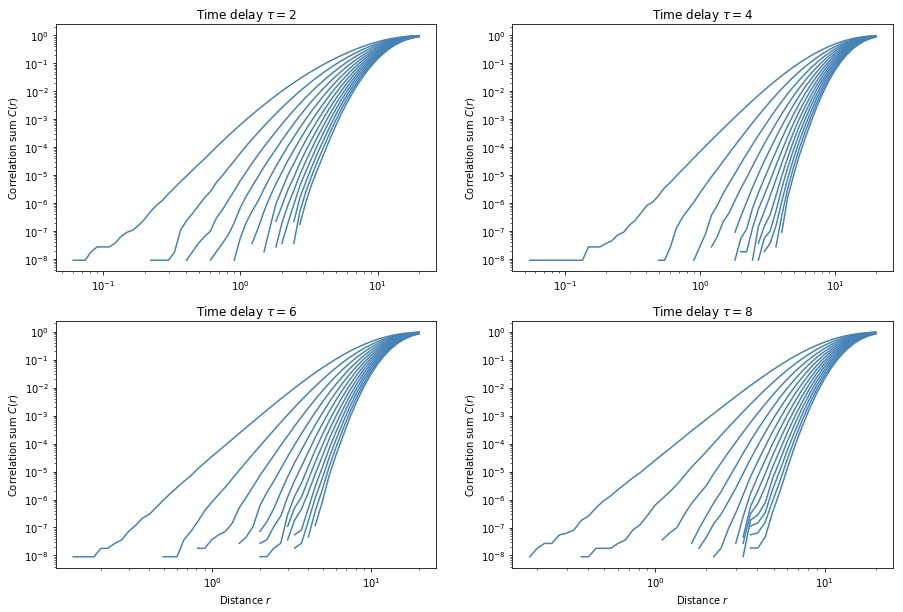
\includegraphics[width=1.0\textwidth]{Images/cr.png} }
  \caption{Normalized correlation sum as a function of radius $r$ for dimensions in range from $5$ to $30$ (from left to right).}
  \label{fig:cr}
\end{figure}

\begin{figure} 
\centering
\noindent\makebox[\textwidth]{%
  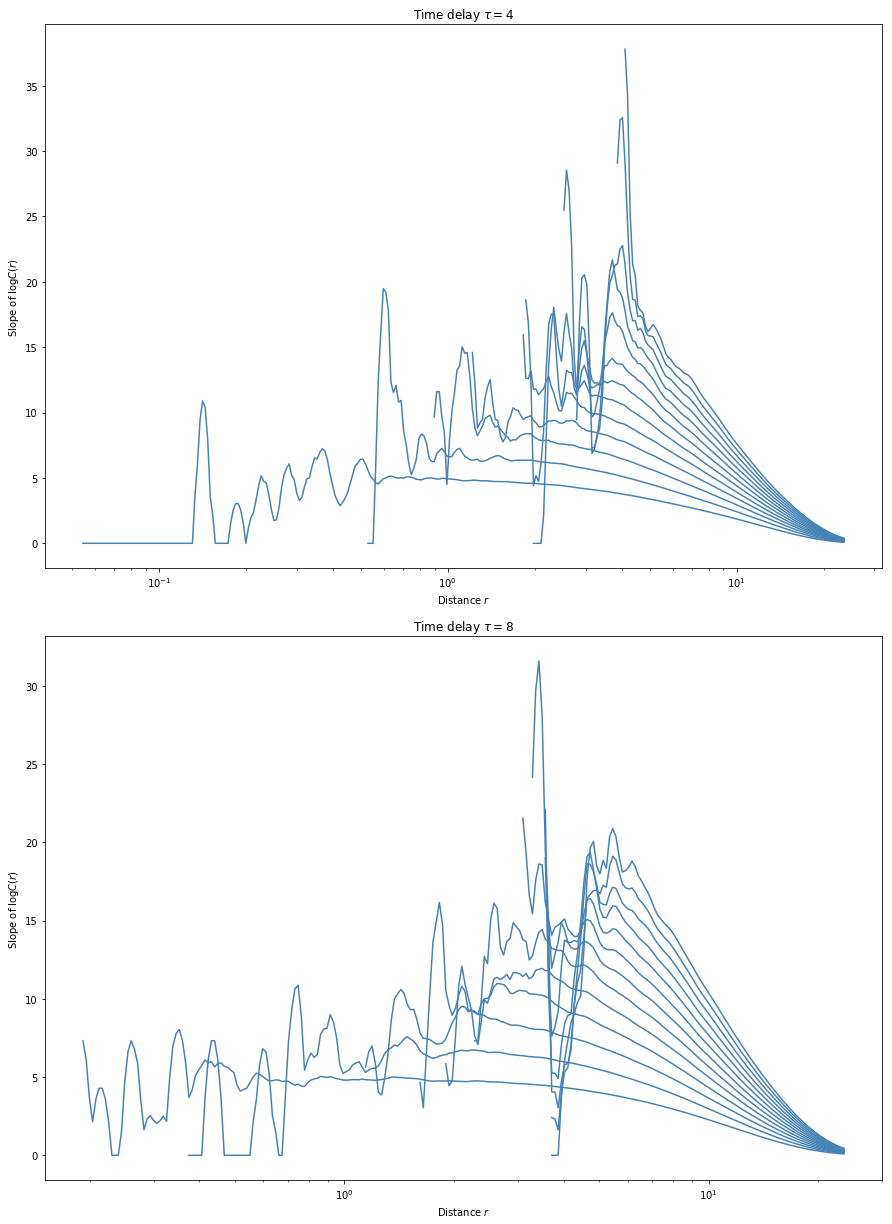
\includegraphics[width=0.95\textwidth]{./Images/local_d_2/large.png} }
  \caption{Local correlation dimension $d_2$ as a function of radius $r$ for dimensions in range from $5$ to $30$ (from bottom to top) and time delays $\tau = 4$ and $\tau = 8$.}
  \label{fig:loc-d2}
\end{figure}

\begin{figure} 
\centering
\noindent\makebox[\textwidth]{%
  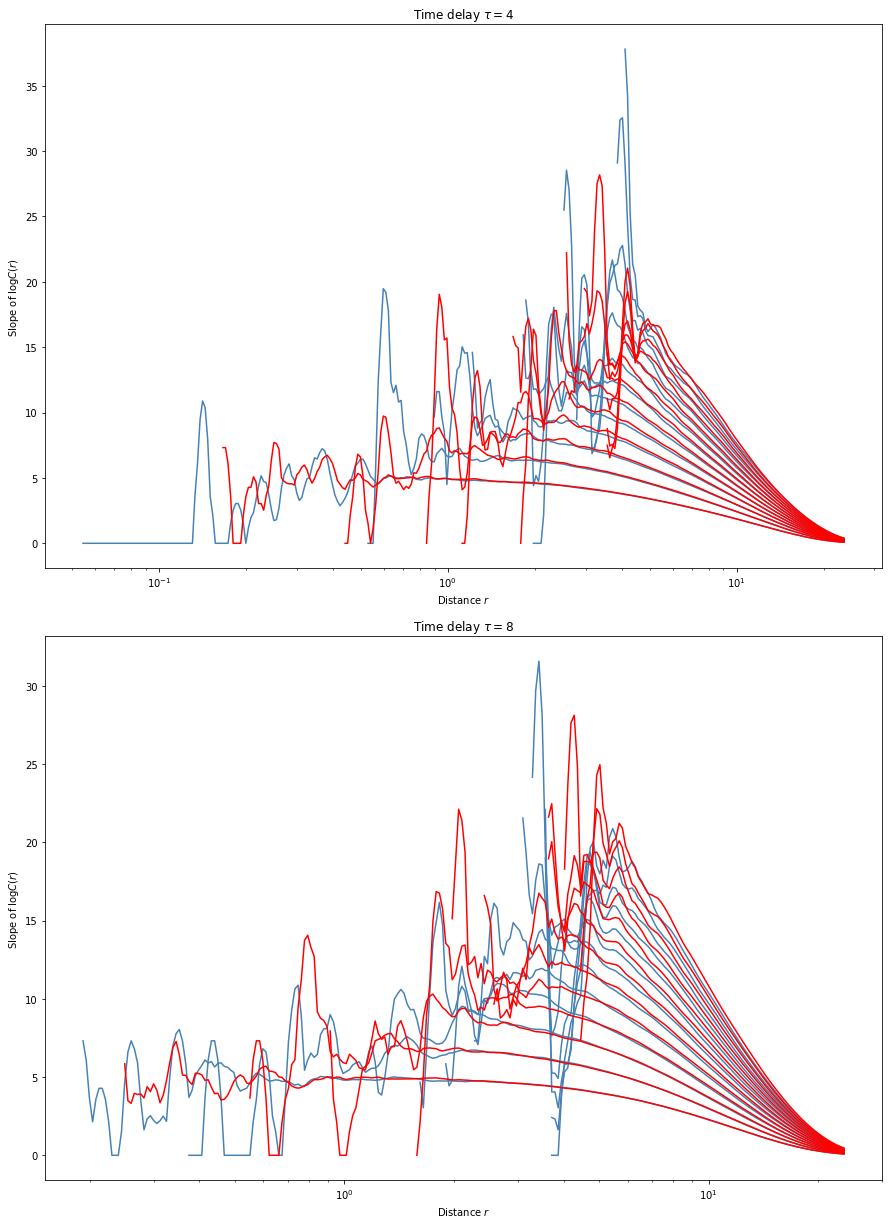
\includegraphics[width=0.95\textwidth]{./Images/local_d_2/large_surr.png} }
  \caption{Local correlation dimension $d_2$ as a function of radius $r$ for dimensions in range from $5$ to $30$ (from bottom to top) and time delays $\tau = 4$ and $\tau = 8$ for the original series (blue) and its surrogate series computed using iAAFT.}
  \label{fig:loc-d2-comp}
\end{figure}

\begin{figure} 
\centering
\noindent\makebox[\textwidth]{%
  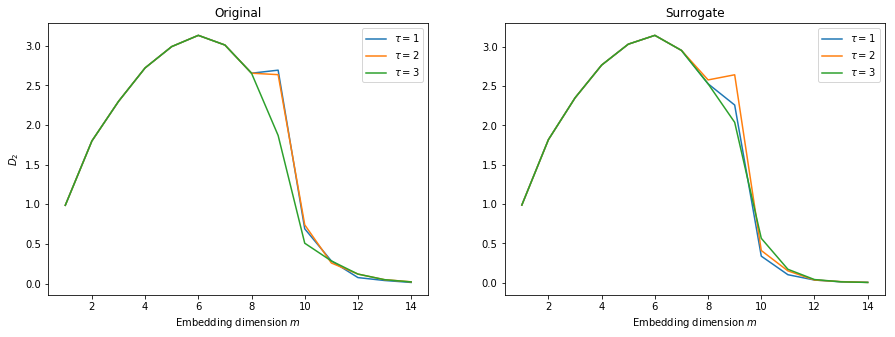
\includegraphics[width=1.0\textwidth]{./Images/em_corrdim.png} }
  \caption{Correlation dimension as function of the embedding dimension $m$.}
\label{fig:em-corrdim}
\end{figure}

\subsection{Detrended fluctuation analysis}
\subsection{Hurst exponent}
\subsection{Higuchi fractal dimension}
\subsection{Sample entropy}

\subsection{Surrogate analysis} \label{sec:surrogate-analysis}

\begin{figure} 
\centering
\noindent\makebox[\textwidth]{%
  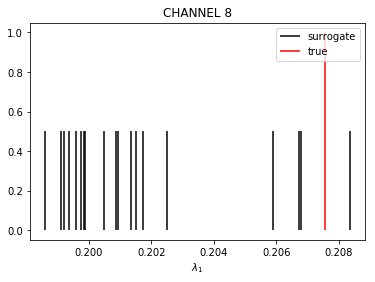
\includegraphics[width=0.5\textwidth]{Images/surr_test.png} }
  \caption{Example distribution of the largest Lyapunov exponent for surrogate data and the original.}
\label{fig:surr-test}
\end{figure}

\section{Analysis of measure distributions between groups} \label{sec:distanal}
\subsection{Before and after treatment}
As the first step of our analysis, we conducted an investigation of the differences in the non-linear measures computed from the signals obtained before and after treatment. The purpose of this inquiry is to determine brain regions and measures affected by treatment. This is warranted by the fact that the patterns in EEG signals tend to be relatively stable over time. \add{This should be cited!} On the other hand, we realize the limitations of this attempt in the case of this study, since each patient recieved personalized method of treatment, and the methods may have differing impact.

We separated the patients into terciles according to the ratio of the depression scores before and after treatment. Out of these three populations, we selected the first and last, containing 46 and 44 samples respectively, to obtain population we call \emph{responding} (responders) to treatment and \emph{non-responding} (non-responders) to treatment. The second tercile was not considered in this analysis to minimize the effect of inaccuracy of the self-reported depression score. Comparison of mean values of individual measures between the two populations can be seen in Figures \ref{fig:respnon1}, \ref{fig:respnon1auto} and \ref{fig:respnon2}. Length of an error bar corresponds to one standard deviation.

For each group, we performed two-sided Kolmogorov-Smirnov test \add{Kruskal is better, redirect to distributions.} for the null hypothesis that the distributions of values computed for measurements before and after treatment are the same. No significant differences in distributions were found for $d_2$ computed using automatic selection of embedding parameters so in this section, we used $\lambda_1$ and $d_2$ computed for $m = 10$, $\tau=3$, $w_t = 50$. Moreover, we found no significant differences in DFA, so we decided to leave it out of this analysis. \info{However, we found that responders had significantly lower $\lambda_1$ computed using these methods in C3 and C4 electrodes ($6.899\pm1.278$ vs. $7.342\pm1.838$ for C3, $6.731\pm1.116$ vs. $7.365\pm1.475$ for C4) on recording performed before treatment.} The results can be seen in Tables \ref{tab:lleba}, \ref{tab:d2ba} and \ref{tab:seba}. 

For all measures computed this way, we found significantly differences in temporal areas, especially T3. The distributions of Largest Lyapunov exponents were also significantly different in the frontal and ``central'' areas, whereas $d_2$ differed mainly in prefrontal areas.\info{Which are associated with depression, but we want to leave that out in this section.} Sample entropy mimics the pattern seen in $\lambda_1$, differing mainly in frontal and ``central'' areas.

We also performed unsupervised analysis of before / after groupds using PCA in 2,3, and 4 dimensions, and compared centroids and mean distances between before and after treatment recording for each group. However, the resulting plots and heatmaps are featureless and thus we will leave them out. The mean distances are also uninformative.

\add[inline]{Change the tables and text to using Kruskal test instead of KS. Justify by saying the distributions are not generally normal.}

\begin{table}[tbp]
\centering
\begin{tabular}{|c|c|c|c|c|}
\hline
\textbf{Channel} & \textbf{Before} & \textbf{After} & \textbf{p-value} & \textbf{Significance} \\ \hline
mean     & 10.151 $\pm$ 0.950 & 9.919 $\pm$ 1.074 & 0.121 &       \\ \hline
std      & 0.628 $\pm$ 0.239 & 0.724 $\pm$ 0.295 & 0.089 &       \\ \hline
FP1      & 9.770 $\pm$ 1.130 & 9.545 $\pm$ 1.287 & 0.432 &       \\ \hline
FP2      & 9.764 $\pm$ 1.186 & 9.565 $\pm$ 1.281 & 0.432 &       \\ \hline
F3       & 9.794 $\pm$ 1.082 & 9.493 $\pm$ 1.177 & 0.065 & *     \\ \hline
F4       & 9.862 $\pm$ 1.090 & 9.413 $\pm$ 1.330 & 0.010 & ***   \\ \hline
C3       & 9.846 $\pm$ 1.068 & 9.579 $\pm$ 1.117 & 0.089 &       \\ \hline
C4       & 9.922 $\pm$ 1.046 & 9.598 $\pm$ 1.196 & 0.033 & **    \\ \hline
P3       & 10.447 $\pm$ 0.865 & 10.291 $\pm$ 1.055 & 0.212 &       \\ \hline
P4       & 10.437 $\pm$ 0.883 & 10.266 $\pm$ 1.046 & 0.832 &       \\ \hline
O1       & 10.539 $\pm$ 1.174 & 10.485 $\pm$ 1.271 & 0.965 &       \\ \hline
O2       & 10.518 $\pm$ 1.198 & 10.409 $\pm$ 1.312 & 0.273 &       \\ \hline
F7       & 10.096 $\pm$ 1.351 & 9.886 $\pm$ 1.402 & 0.432 &       \\ \hline
F8       & 10.118 $\pm$ 1.297 & 9.785 $\pm$ 1.545 & 0.273 &       \\ \hline
T3       & 9.872 $\pm$ 1.308 & 9.387 $\pm$ 1.544 & 0.000 & ***   \\ \hline
T4       & 9.842 $\pm$ 1.317 & 9.449 $\pm$ 1.534 & 0.065 & *     \\ \hline
T5       & 10.506 $\pm$ 1.092 & 10.329 $\pm$ 1.262 & 0.273 &       \\ \hline
T6       & 10.584 $\pm$ 1.087 & 10.380 $\pm$ 1.189 & 0.347 &       \\ \hline
Fz       & 10.257 $\pm$ 1.004 & 10.117 $\pm$ 1.096 & 0.161 &       \\ \hline
Cz       & 10.204 $\pm$ 0.906 & 10.075 $\pm$ 0.998 & 0.273 &       \\ \hline
Pz       & 10.490 $\pm$ 0.897 & 10.408 $\pm$ 1.032 & 0.735 &       \\ \hline
\end{tabular}
\caption{Mean values of $\lambda_1$ of all patients before and after treatment.}
\label{tab:lleba}
\end{table}

\begin{table}[tbp]
\centering
\begin{tabular}{|c|c|c|c|c|}
\hline
\textbf{Channel} & \textbf{Before} & \textbf{After} & \textbf{p-value} & \textbf{Significance} \\ \hline
mean     & 7.522 $\pm$ 0.441 & 7.593 $\pm$ 0.433 & 0.481 &       \\ \hline
std      & 0.383 $\pm$ 0.125 & 0.414 $\pm$ 0.165 & 0.071 & *     \\ \hline
FP1      & 7.812 $\pm$ 0.611 & 7.880 $\pm$ 0.704 & 0.387 &       \\ \hline
FP2      & 7.826 $\pm$ 0.650 & 7.935 $\pm$ 0.790 & 0.035 & **    \\ \hline
F3       & 7.594 $\pm$ 0.592 & 7.681 $\pm$ 0.586 & 0.179 &       \\ \hline
F4       & 7.639 $\pm$ 0.602 & 7.726 $\pm$ 0.582 & 0.387 &       \\ \hline
C3       & 7.342 $\pm$ 0.592 & 7.395 $\pm$ 0.591 & 0.585 &       \\ \hline
C4       & 7.334 $\pm$ 0.550 & 7.412 $\pm$ 0.574 & 0.387 &       \\ \hline
P3       & 7.274 $\pm$ 0.515 & 7.319 $\pm$ 0.522 & 0.305 &       \\ \hline
P4       & 7.325 $\pm$ 0.573 & 7.349 $\pm$ 0.506 & 0.888 &       \\ \hline
O1       & 7.539 $\pm$ 0.566 & 7.543 $\pm$ 0.524 & 0.987 &       \\ \hline
O2       & 7.516 $\pm$ 0.518 & 7.569 $\pm$ 0.547 & 0.387 &       \\ \hline
F7       & 7.680 $\pm$ 0.530 & 7.812 $\pm$ 0.550 & 0.305 &       \\ \hline
F8       & 7.702 $\pm$ 0.534 & 7.822 $\pm$ 0.565 & 0.179 &       \\ \hline
T3       & 7.669 $\pm$ 0.585 & 7.877 $\pm$ 0.624 & 0.011 & ***   \\ \hline
T4       & 7.684 $\pm$ 0.588 & 7.840 $\pm$ 0.556 & 0.024 & **    \\ \hline
T5       & 7.556 $\pm$ 0.523 & 7.593 $\pm$ 0.481 & 0.585 &       \\ \hline
T6       & 7.536 $\pm$ 0.518 & 7.593 $\pm$ 0.483 & 0.585 &       \\ \hline
Fz       & 7.339 $\pm$ 0.535 & 7.350 $\pm$ 0.525 & 0.987 &       \\ \hline
Cz       & 7.359 $\pm$ 0.566 & 7.354 $\pm$ 0.533 & 0.998 &       \\ \hline
Pz       & 7.199 $\pm$ 0.494 & 7.210 $\pm$ 0.543 & 0.888 &       \\ \hline
\end{tabular}
\caption{Mean values of $d_2$ of all patients before and after treatment.}
\label{tab:d2ba}
\end{table}

\begin{table}[tbp]
\centering
\begin{tabular}{|c|c|c|c|c|}
\hline
\textbf{Channel} & \textbf{Before} & \textbf{After} & \textbf{p-value} & \textbf{Significance} \\ \hline
mean     & 0.761 $\pm$ 0.108 & 0.790 $\pm$ 0.130 & 0.240 &       \\ \hline
std      & 0.071 $\pm$ 0.040 & 0.086 $\pm$ 0.048 & 0.094 &       \\ \hline
FP1      & 0.804 $\pm$ 0.149 & 0.837 $\pm$ 0.176 & 0.403 &       \\ \hline
FP2      & 0.802 $\pm$ 0.156 & 0.830 $\pm$ 0.175 & 0.403 &       \\ \hline
F3       & 0.800 $\pm$ 0.132 & 0.839 $\pm$ 0.156 & 0.179 &       \\ \hline
F4       & 0.790 $\pm$ 0.137 & 0.842 $\pm$ 0.168 & 0.046 & **    \\ \hline
C3       & 0.793 $\pm$ 0.122 & 0.825 $\pm$ 0.147 & 0.314 &       \\ \hline
C4       & 0.781 $\pm$ 0.126 & 0.821 $\pm$ 0.151 & 0.046 & **    \\ \hline
P3       & 0.720 $\pm$ 0.087 & 0.740 $\pm$ 0.115 & 0.619 &       \\ \hline
P4       & 0.720 $\pm$ 0.093 & 0.736 $\pm$ 0.116 & 0.975 &       \\ \hline
O1       & 0.707 $\pm$ 0.113 & 0.718 $\pm$ 0.134 & 0.734 &       \\ \hline
O2       & 0.712 $\pm$ 0.113 & 0.732 $\pm$ 0.154 & 0.314 &       \\ \hline
F7       & 0.786 $\pm$ 0.163 & 0.811 $\pm$ 0.176 & 0.619 &       \\ \hline
F8       & 0.781 $\pm$ 0.156 & 0.821 $\pm$ 0.195 & 0.403 &       \\ \hline
T3       & 0.806 $\pm$ 0.160 & 0.867 $\pm$ 0.197 & 0.006 & ***   \\ \hline
T4       & 0.812 $\pm$ 0.167 & 0.861 $\pm$ 0.197 & 0.131 &       \\ \hline
T5       & 0.723 $\pm$ 0.110 & 0.743 $\pm$ 0.133 & 0.403 &       \\ \hline
T6       & 0.714 $\pm$ 0.112 & 0.729 $\pm$ 0.123 & 0.506 &       \\ \hline
Fz       & 0.747 $\pm$ 0.107 & 0.762 $\pm$ 0.124 & 0.506 &       \\ \hline
Cz       & 0.756 $\pm$ 0.096 & 0.767 $\pm$ 0.110 & 0.840 &       \\ \hline
Pz       & 0.716 $\pm$ 0.093 & 0.728 $\pm$ 0.113 & 0.996 &       \\ \hline
\end{tabular}
\caption{Mean values of sample entropy of all patients before and after treatment.}
\label{tab:seba}
\end{table}

\begin{table}[tbp]
\centering
\tiny
  \parbox{.45\linewidth}{
\begin{tabular}{|c|c|c|c|c|}
\hline
\textbf{Channel} & \textbf{Before} & \textbf{After} & \textbf{p-value} & \textbf{Significance} \\ \hline
mean     & 9.994 $\pm$ 0.890 & 9.655 $\pm$ 1.064 & 0.022 & **    \\ \hline
std      & 0.639 $\pm$ 0.229 & 0.701 $\pm$ 0.267 & 0.452 &       \\ \hline
FP1      & 9.599 $\pm$ 1.086 & 9.335 $\pm$ 1.360 & 0.625 &       \\ \hline
FP2      & 9.590 $\pm$ 1.090 & 9.281 $\pm$ 1.293 & 0.308 &       \\ \hline
F3       & 9.588 $\pm$ 1.119 & 9.190 $\pm$ 1.190 & 0.123 &       \\ \hline
F4       & 9.682 $\pm$ 0.999 & 9.199 $\pm$ 1.339 & 0.072 & *     \\ \hline
C3       & 9.690 $\pm$ 1.065 & 9.349 $\pm$ 1.111 & 0.072 & *     \\ \hline
C4       & 9.827 $\pm$ 1.052 & 9.407 $\pm$ 1.221 & 0.041 & **    \\ \hline
P3       & 10.294 $\pm$ 0.797 & 10.032 $\pm$ 1.050 & 0.072 & *     \\ \hline
P4       & 10.265 $\pm$ 0.873 & 10.004 $\pm$ 1.104 & 0.308 &       \\ \hline
O1       & 10.343 $\pm$ 1.081 & 10.117 $\pm$ 1.176 & 0.452 &       \\ \hline
O2       & 10.261 $\pm$ 1.160 & 9.961 $\pm$ 1.212 & 0.123 &       \\ \hline
F7       & 9.998 $\pm$ 1.324 & 9.682 $\pm$ 1.419 & 0.199 &       \\ \hline
F8       & 9.991 $\pm$ 1.170 & 9.659 $\pm$ 1.492 & 0.308 &       \\ \hline
T3       & 9.789 $\pm$ 1.387 & 9.172 $\pm$ 1.492 & 0.005 & ***   \\ \hline
T4       & 9.703 $\pm$ 1.261 & 9.164 $\pm$ 1.403 & 0.022 & **    \\ \hline
T5       & 10.370 $\pm$ 1.091 & 10.073 $\pm$ 1.214 & 0.011 & ***   \\ \hline
T6       & 10.335 $\pm$ 0.954 & 10.021 $\pm$ 1.166 & 0.123 &       \\ \hline
Fz       & 10.096 $\pm$ 0.970 & 9.849 $\pm$ 1.126 & 0.072 & *     \\ \hline
Cz       & 10.150 $\pm$ 0.886 & 9.847 $\pm$ 1.006 & 0.123 &       \\ \hline
Pz       & 10.318 $\pm$ 0.805 & 10.113 $\pm$ 1.062 & 0.801 &       \\ \hline
\end{tabular}
}
\hfill
  \parbox{.45\linewidth}{
\begin{tabular}{|c|c|c|c|c|}
\hline
\textbf{Channel} & \textbf{Before} & \textbf{After} & \textbf{p-value} & \textbf{Significance} \\ \hline
mean     & 10.400 $\pm$ 0.969 & 10.015 $\pm$ 1.088 & 0.423 &       \\ \hline
std      & 0.623 $\pm$ 0.260 & 0.813 $\pm$ 0.370 & 0.018 & ***   \\ \hline
FP1      & 10.034 $\pm$ 1.166 & 9.510 $\pm$ 1.325 & 0.108 &       \\ \hline
FP2      & 10.045 $\pm$ 1.196 & 9.752 $\pm$ 1.269 & 0.778 &       \\ \hline
F3       & 10.116 $\pm$ 1.034 & 9.619 $\pm$ 1.200 & 0.108 &       \\ \hline
F4       & 10.098 $\pm$ 1.146 & 9.343 $\pm$ 1.364 & 0.034 & **    \\ \hline
C3       & 10.160 $\pm$ 1.010 & 9.585 $\pm$ 1.147 & 0.018 & ***   \\ \hline
C4       & 10.162 $\pm$ 1.060 & 9.681 $\pm$ 1.170 & 0.062 & *     \\ \hline
P3       & 10.711 $\pm$ 0.874 & 10.468 $\pm$ 1.065 & 0.423 &       \\ \hline
P4       & 10.720 $\pm$ 0.897 & 10.453 $\pm$ 1.005 & 0.595 &       \\ \hline
O1       & 10.765 $\pm$ 1.292 & 10.772 $\pm$ 1.352 & 0.924 &       \\ \hline
O2       & 10.823 $\pm$ 1.242 & 10.604 $\pm$ 1.434 & 0.595 &       \\ \hline
F7       & 10.234 $\pm$ 1.340 & 9.875 $\pm$ 1.459 & 0.282 &       \\ \hline
F8       & 10.307 $\pm$ 1.405 & 9.556 $\pm$ 1.715 & 0.108 &       \\ \hline
T3       & 10.073 $\pm$ 1.207 & 9.292 $\pm$ 1.602 & 0.004 & ***   \\ \hline
T4       & 10.018 $\pm$ 1.431 & 9.394 $\pm$ 1.726 & 0.179 &       \\ \hline
T5       & 10.709 $\pm$ 1.140 & 10.490 $\pm$ 1.301 & 0.778 &       \\ \hline
T6       & 10.933 $\pm$ 1.072 & 10.649 $\pm$ 1.219 & 0.778 &       \\ \hline
Fz       & 10.568 $\pm$ 0.951 & 10.327 $\pm$ 1.024 & 0.423 &       \\ \hline
Cz       & 10.383 $\pm$ 0.867 & 10.291 $\pm$ 0.939 & 0.924 &       \\ \hline
Pz       & 10.744 $\pm$ 0.894 & 10.630 $\pm$ 1.023 & 0.423 &       \\ \hline
\end{tabular}
}
\caption{Mean values of $\lambda_1$ of responding / non-responding patients before and after treatment.}
\label{tab:llebaresp}
\end{table}

\begin{table}[tbp]
\centering
\tiny
  \parbox{.45\linewidth}{
\begin{tabular}{|c|c|c|c|c|}
\hline
\textbf{Channel} & \textbf{Before} & \textbf{After} & \textbf{p-value} & \textbf{Significance} \\ \hline
mean     & 7.536 $\pm$ 0.394 & 7.585 $\pm$ 0.465 & 0.765 &       \\ \hline
std      & 0.401 $\pm$ 0.121 & 0.400 $\pm$ 0.134 & 0.917 &       \\ \hline
FP1      & 7.851 $\pm$ 0.588 & 7.841 $\pm$ 0.751 & 0.580 &       \\ \hline
FP2      & 7.921 $\pm$ 0.647 & 7.903 $\pm$ 0.553 & 0.580 &       \\ \hline
F3       & 7.614 $\pm$ 0.579 & 7.714 $\pm$ 0.634 & 0.765 &       \\ \hline
F4       & 7.640 $\pm$ 0.575 & 7.696 $\pm$ 0.591 & 0.408 &       \\ \hline
C3       & 7.399 $\pm$ 0.575 & 7.416 $\pm$ 0.659 & 0.989 &       \\ \hline
C4       & 7.303 $\pm$ 0.481 & 7.378 $\pm$ 0.615 & 0.765 &       \\ \hline
P3       & 7.247 $\pm$ 0.488 & 7.288 $\pm$ 0.552 & 0.580 &       \\ \hline
P4       & 7.338 $\pm$ 0.510 & 7.337 $\pm$ 0.543 & 0.765 &       \\ \hline
O1       & 7.554 $\pm$ 0.479 & 7.593 $\pm$ 0.571 & 0.917 &       \\ \hline
O2       & 7.539 $\pm$ 0.464 & 7.599 $\pm$ 0.560 & 0.765 &       \\ \hline
F7       & 7.662 $\pm$ 0.585 & 7.797 $\pm$ 0.601 & 0.269 &       \\ \hline
F8       & 7.717 $\pm$ 0.469 & 7.762 $\pm$ 0.574 & 0.408 &       \\ \hline
T3       & 7.694 $\pm$ 0.524 & 7.902 $\pm$ 0.636 & 0.269 &       \\ \hline
T4       & 7.682 $\pm$ 0.563 & 7.826 $\pm$ 0.522 & 0.100 &       \\ \hline
T5       & 7.606 $\pm$ 0.532 & 7.589 $\pm$ 0.477 & 0.765 &       \\ \hline
T6       & 7.578 $\pm$ 0.460 & 7.625 $\pm$ 0.485 & 0.765 &       \\ \hline
Fz       & 7.335 $\pm$ 0.522 & 7.340 $\pm$ 0.571 & 0.989 &       \\ \hline
Cz       & 7.321 $\pm$ 0.574 & 7.354 $\pm$ 0.532 & 0.917 &       \\ \hline
Pz       & 7.188 $\pm$ 0.451 & 7.162 $\pm$ 0.538 & 0.765 &       \\ \hline
\end{tabular}
}
\hfill
  \parbox{.45\linewidth}{
\begin{tabular}{|c|c|c|c|c|}
\hline
\textbf{Channel} & \textbf{Before} & \textbf{After} & \textbf{p-value} & \textbf{Significance} \\ \hline
mean     & 7.483 $\pm$ 0.432 & 7.648 $\pm$ 0.369 & 0.548 &       \\ \hline
std      & 0.366 $\pm$ 0.116 & 0.450 $\pm$ 0.162 & 0.048 & **    \\ \hline
FP1      & 7.709 $\pm$ 0.552 & 7.984 $\pm$ 0.658 & 0.149 &       \\ \hline
FP2      & 7.749 $\pm$ 0.582 & 7.909 $\pm$ 0.544 & 0.244 &       \\ \hline
F3       & 7.517 $\pm$ 0.576 & 7.717 $\pm$ 0.548 & 0.244 &       \\ \hline
F4       & 7.585 $\pm$ 0.621 & 7.886 $\pm$ 0.603 & 0.086 &       \\ \hline
C3       & 7.271 $\pm$ 0.579 & 7.427 $\pm$ 0.583 & 0.377 &       \\ \hline
C4       & 7.335 $\pm$ 0.561 & 7.435 $\pm$ 0.527 & 0.738 &       \\ \hline
P3       & 7.272 $\pm$ 0.474 & 7.392 $\pm$ 0.488 & 0.548 &       \\ \hline
P4       & 7.268 $\pm$ 0.457 & 7.417 $\pm$ 0.518 & 0.548 &       \\ \hline
O1       & 7.510 $\pm$ 0.693 & 7.530 $\pm$ 0.484 & 0.548 &       \\ \hline
O2       & 7.494 $\pm$ 0.533 & 7.623 $\pm$ 0.563 & 0.377 &       \\ \hline
F7       & 7.643 $\pm$ 0.419 & 7.874 $\pm$ 0.486 & 0.048 & **    \\ \hline
F8       & 7.651 $\pm$ 0.557 & 7.914 $\pm$ 0.554 & 0.012 & ***   \\ \hline
T3       & 7.616 $\pm$ 0.582 & 8.032 $\pm$ 0.646 & 0.012 & ***   \\ \hline
T4       & 7.687 $\pm$ 0.604 & 7.984 $\pm$ 0.648 & 0.086 &       \\ \hline
T5       & 7.517 $\pm$ 0.518 & 7.625 $\pm$ 0.441 & 0.548 &       \\ \hline
T6       & 7.488 $\pm$ 0.494 & 7.613 $\pm$ 0.493 & 0.377 &       \\ \hline
Fz       & 7.287 $\pm$ 0.509 & 7.359 $\pm$ 0.459 & 0.548 &       \\ \hline
Cz       & 7.380 $\pm$ 0.536 & 7.326 $\pm$ 0.490 & 0.902 &       \\ \hline
Pz       & 7.195 $\pm$ 0.498 & 7.262 $\pm$ 0.499 & 0.548 &       \\ \hline
\end{tabular}
}
\caption{Mean values of $d_2$ of responding / non-respoding patients before and after treatment.}
\label{tab:d2baresp}
\end{table}

\begin{table}[tbp]
\centering
\tiny
  \parbox{.45\linewidth}{
\begin{tabular}{|c|c|c|c|c|}
\hline
\textbf{Channel} & \textbf{Before} & \textbf{After} & \textbf{p-value} & \textbf{Significance} \\ \hline
mean     & 0.768 $\pm$ 0.093 & 0.811 $\pm$ 0.107 & 0.086 &       \\ \hline
std      & 0.078 $\pm$ 0.039 & 0.093 $\pm$ 0.047 & 0.377 &       \\ \hline
FP1      & 0.816 $\pm$ 0.156 & 0.866 $\pm$ 0.178 & 0.548 &       \\ \hline
FP2      & 0.819 $\pm$ 0.158 & 0.866 $\pm$ 0.171 & 0.377 &       \\ \hline
F3       & 0.815 $\pm$ 0.128 & 0.872 $\pm$ 0.145 & 0.086 &       \\ \hline
F4       & 0.801 $\pm$ 0.126 & 0.868 $\pm$ 0.160 & 0.048 & **    \\ \hline
C3       & 0.796 $\pm$ 0.107 & 0.841 $\pm$ 0.123 & 0.149 &       \\ \hline
C4       & 0.780 $\pm$ 0.112 & 0.844 $\pm$ 0.129 & 0.012 & ***   \\ \hline
P3       & 0.718 $\pm$ 0.075 & 0.744 $\pm$ 0.089 & 0.548 &       \\ \hline
P4       & 0.722 $\pm$ 0.089 & 0.751 $\pm$ 0.103 & 0.548 &       \\ \hline
O1       & 0.704 $\pm$ 0.074 & 0.738 $\pm$ 0.111 & 0.244 &       \\ \hline
O2       & 0.725 $\pm$ 0.094 & 0.746 $\pm$ 0.116 & 0.149 &       \\ \hline
F7       & 0.790 $\pm$ 0.166 & 0.837 $\pm$ 0.168 & 0.149 &       \\ \hline
F8       & 0.786 $\pm$ 0.138 & 0.845 $\pm$ 0.190 & 0.548 &       \\ \hline
T3       & 0.813 $\pm$ 0.163 & 0.894 $\pm$ 0.181 & 0.012 & ***   \\ \hline
T4       & 0.828 $\pm$ 0.165 & 0.886 $\pm$ 0.162 & 0.048 & **    \\ \hline
T5       & 0.722 $\pm$ 0.078 & 0.762 $\pm$ 0.110 & 0.086 &       \\ \hline
T6       & 0.723 $\pm$ 0.094 & 0.752 $\pm$ 0.090 & 0.086 &       \\ \hline
Fz       & 0.758 $\pm$ 0.094  & 0.782 $\pm$ 0.109 & 0.244 &       \\ \hline
Cz       & 0.760 $\pm$ 0.082 & 0.783 $\pm$ 0.089 & 0.377 &       \\ \hline
Pz       & 0.724 $\pm$ 0.090 & 0.742 $\pm$ 0.103 & 0.902 &       \\ \hline
\end{tabular}
}
\hfill
  \parbox{.45\linewidth}{
\begin{tabular}{|c|c|c|c|c|}
\hline
\textbf{Channel} & \textbf{Before} & \textbf{After} & \textbf{p-value} & \textbf{Significance} \\ \hline
mean     & 0.757 $\pm$ 0.113 & 0.798 $\pm$ 0.137 & 0.676 &       \\ \hline
std      & 0.067 $\pm$ 0.044 & 0.095 $\pm$ 0.057 & 0.061 & *     \\ \hline
FP1      & 0.796 $\pm$ 0.137 & 0.850 $\pm$ 0.178 & 0.479 &       \\ \hline
FP2      & 0.799 $\pm$ 0.146 & 0.823 $\pm$ 0.162 & 0.975 &       \\ \hline
F3       & 0.783 $\pm$ 0.130 & 0.843 $\pm$ 0.163 & 0.479 &       \\ \hline
F4       & 0.782 $\pm$ 0.137 & 0.863 $\pm$ 0.169 & 0.111 &       \\ \hline
C3       & 0.780 $\pm$ 0.128 & 0.826 $\pm$ 0.157 & 0.193 &       \\ \hline
C4       & 0.774 $\pm$ 0.131 & 0.820 $\pm$ 0.153 & 0.193 &       \\ \hline
P3       & 0.713 $\pm$ 0.092 & 0.747 $\pm$ 0.134 & 0.676 &       \\ \hline
P4       & 0.713 $\pm$ 0.092 & 0.735 $\pm$ 0.130 & 0.975 &       \\ \hline
O1       & 0.715 $\pm$ 0.130 & 0.723 $\pm$ 0.159 & 0.975 &       \\ \hline
O2       & 0.716 $\pm$ 0.130 & 0.750 $\pm$ 0.201 & 0.975 &       \\ \hline
F7       & 0.794 $\pm$ 0.167 & 0.824 $\pm$ 0.186 & 0.314 &       \\ \hline
F8       & 0.784 $\pm$ 0.172 & 0.850 $\pm$ 0.207 & 0.314 &       \\ \hline
T3       & 0.802 $\pm$ 0.159 & 0.901 $\pm$ 0.211 & 0.031 & **    \\ \hline
T4       & 0.807 $\pm$ 0.176 & 0.887 $\pm$ 0.222 & 0.193 &       \\ \hline
T5       & 0.722 $\pm$ 0.123 & 0.747 $\pm$ 0.152 & 0.863 &       \\ \hline
T6       & 0.709 $\pm$ 0.127 & 0.721 $\pm$ 0.140 & 0.975 &       \\ \hline
Fz       & 0.731 $\pm$ 0.104 & 0.757 $\pm$ 0.124 & 0.314 &       \\ \hline
Cz       & 0.751 $\pm$ 0.093 & 0.757 $\pm$ 0.105 & 0.975 &       \\ \hline
Pz       & 0.713 $\pm$ 0.092 & 0.730 $\pm$ 0.121 & 0.863 &       \\ \hline
\end{tabular}
}
\caption{Mean values of sample entropy of responding / non-responding patients before and after treatment.}
\label{tab:sebaresp}
\end{table}

\begin{landscape}
  \begin{figure} 
  \centering
  \noindent\makebox[\textwidth]{%
    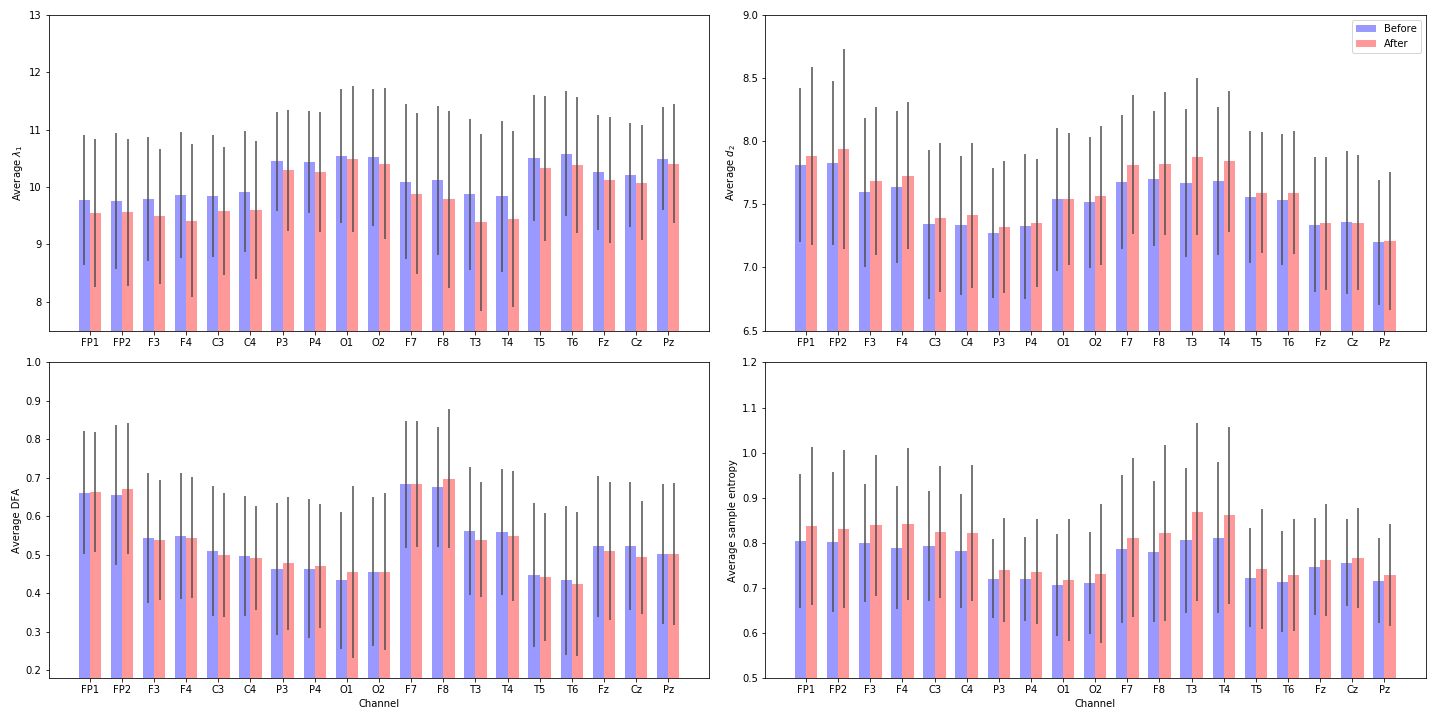
\includegraphics[width=1.4\textwidth]{./Images/bars/bef_aft.png} }
    \caption{Values of individual measures computed before and after treatment.}
   \label{fig:befaft}
  \end{figure}

  \begin{figure} 
  \centering
  \noindent\makebox[\textwidth]{%
    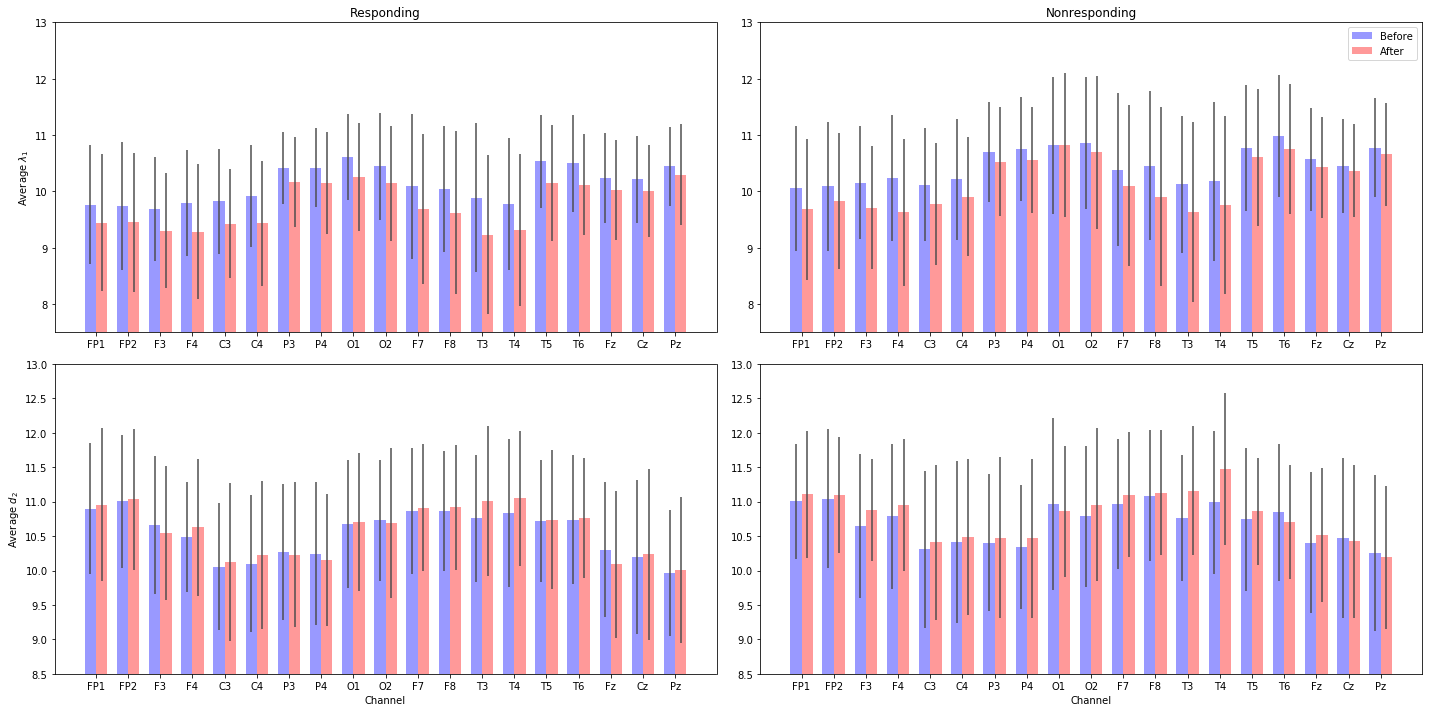
\includegraphics[width=1.4\textwidth]{./Images/bars/resp_non1.png} }
    \caption{Comparison of mean values of largest Lyapunov exponent and correlation dimension between responders and non-responders computed using embedding dimension $m=10$ and time delay $\tau=3$.}
   \label{fig:respnon1}
  \end{figure}

  \begin{figure} 
  \centering
  \noindent\makebox[\textwidth]{%
    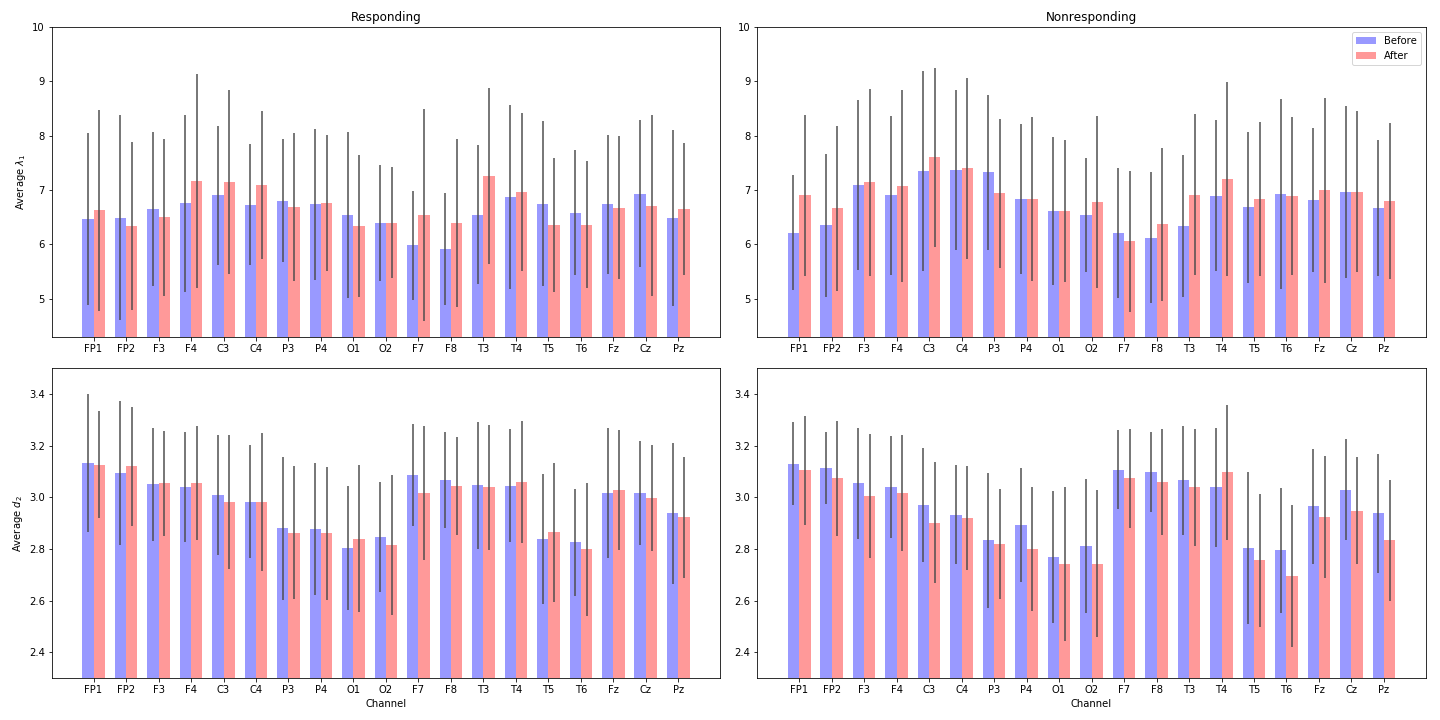
\includegraphics[width=1.4\textwidth]{./Images/bars/resp_non1_auto.png} }
    \caption{Comparison of mean values of largest Lyapunov exponent and correlation dimension between responders and non-responders computed using automatic procedure described in Section .}
   \label{fig:respnon1auto}
  \end{figure}

  \begin{figure} 
  \centering
  \noindent\makebox[\textwidth]{%
    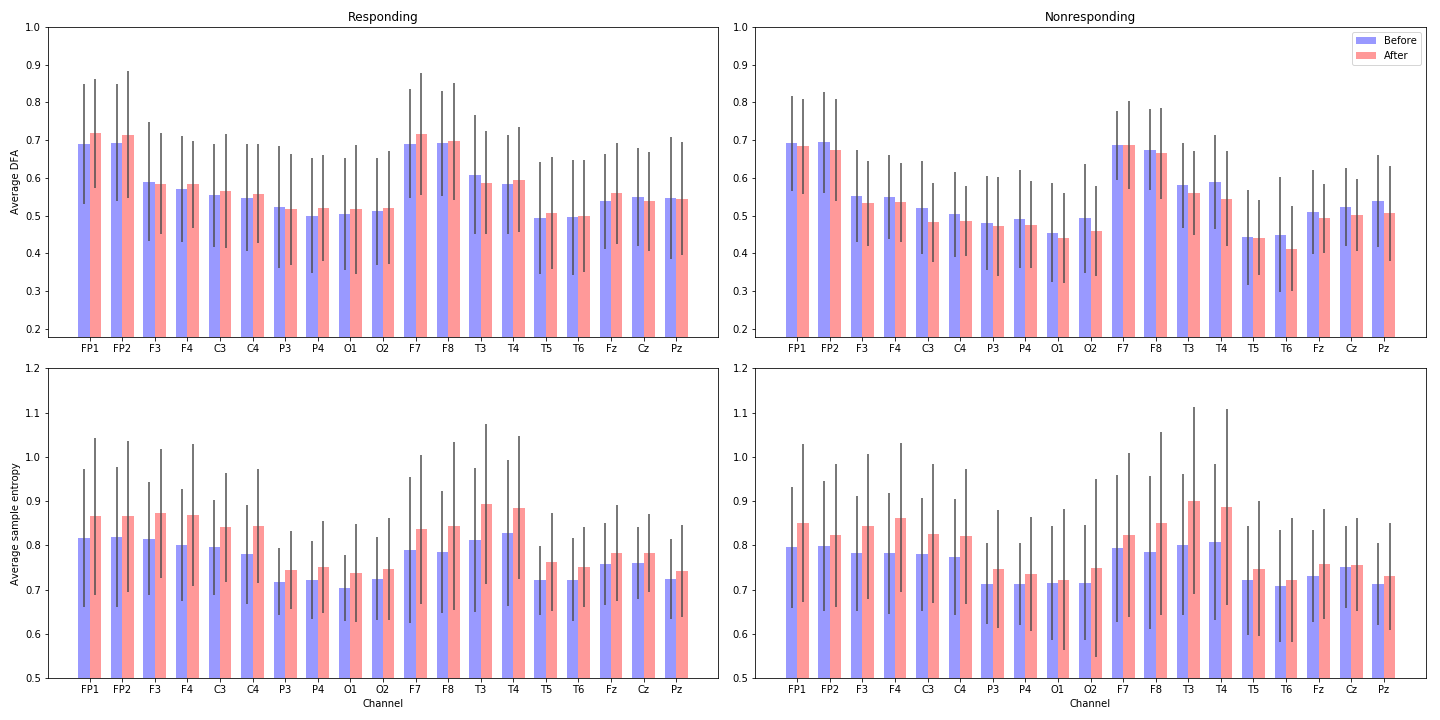
\includegraphics[width=1.4\textwidth]{./Images/bars/resp_non2.png} }
    \caption{Comparison of mean values of computed detrended fluctuation analysis and sample entropy between responders and non-responders.}
   \label{fig:respnon2}
  \end{figure}
\end{landscape}

\subsection{Low and high depression score}
\info[inline]{Here, we have to explain limitations of training classifiers on this test. There is no healthy group. The effect of depression score is meddled with the effect of drugs in after treatment measurements. But still, there are correlations. The goal of this is to inform and maybe interpret the results of classification, and which measures show correlations and how they are distributed between groups, which is inherently important and relevant for eventual interpretation.}
\begin{figure} 
\centering
\noindent\makebox[\textwidth]{%
  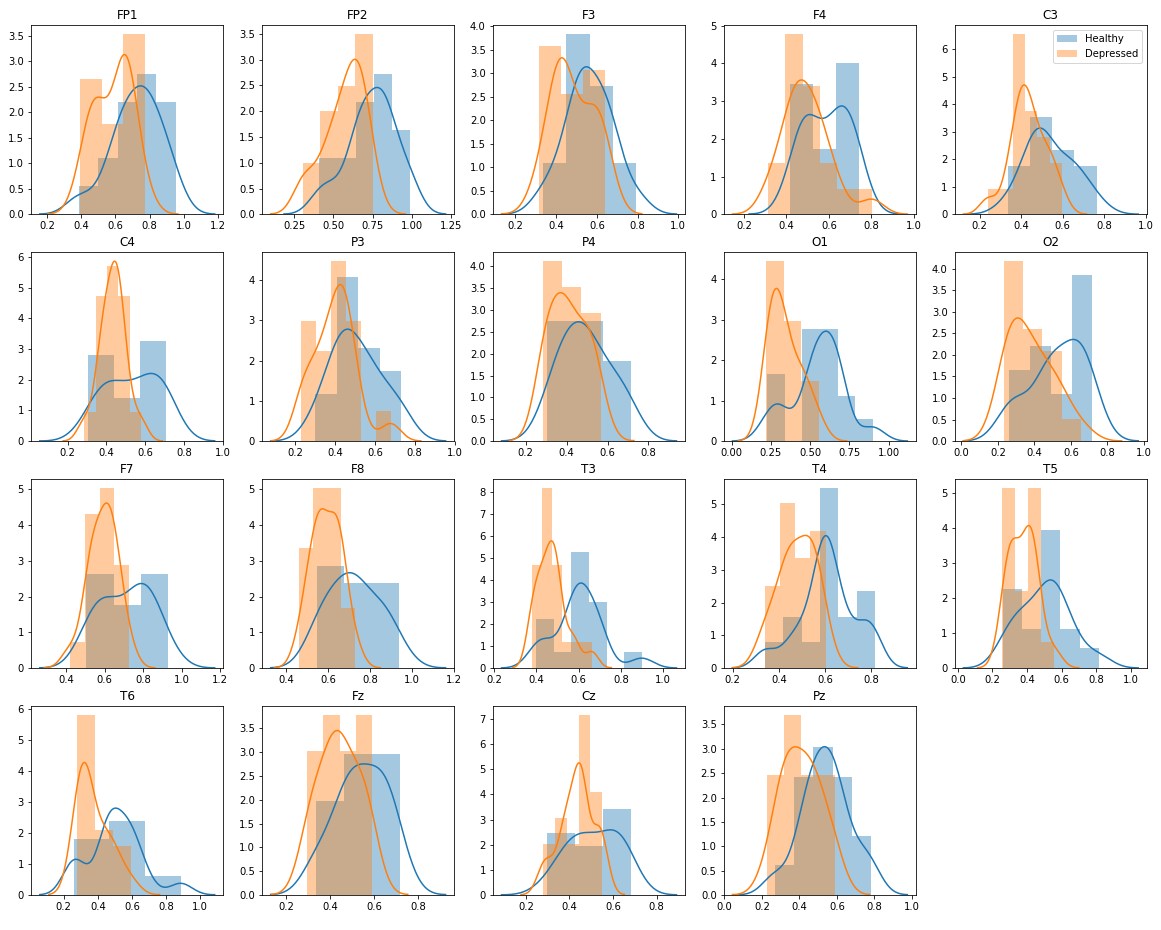
\includegraphics[width=1\textwidth]{./Images/dists/dfadepdist.png} }
  \caption{Distributions of DFA between healthy and depressed patients. Healthy patients seem to have, on average, lower values of DFA, and the distributions are not generally normal.}
 \label{fig:dfadepdist}
\end{figure}

\begin{figure} 
\centering
\noindent\makebox[\textwidth]{%
  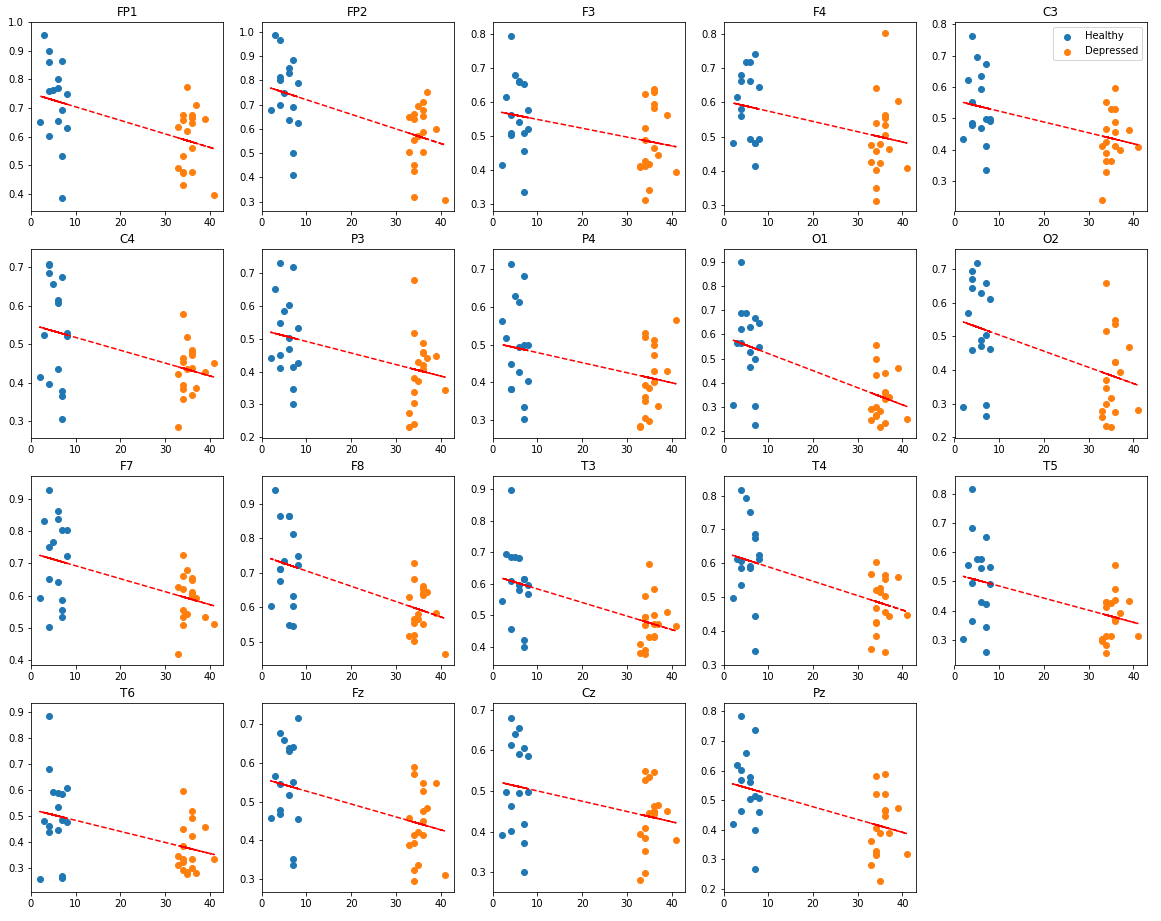
\includegraphics[width=1\textwidth]{./Images/dists/dfadepcorr.png} }
  \caption{Trend of values of DFA as a function of depression score. For all channels, correlation is significantly ($p$ < 0.05) negative.}
\end{figure}

\begin{figure} 
\centering
\noindent\makebox[\textwidth]{%
  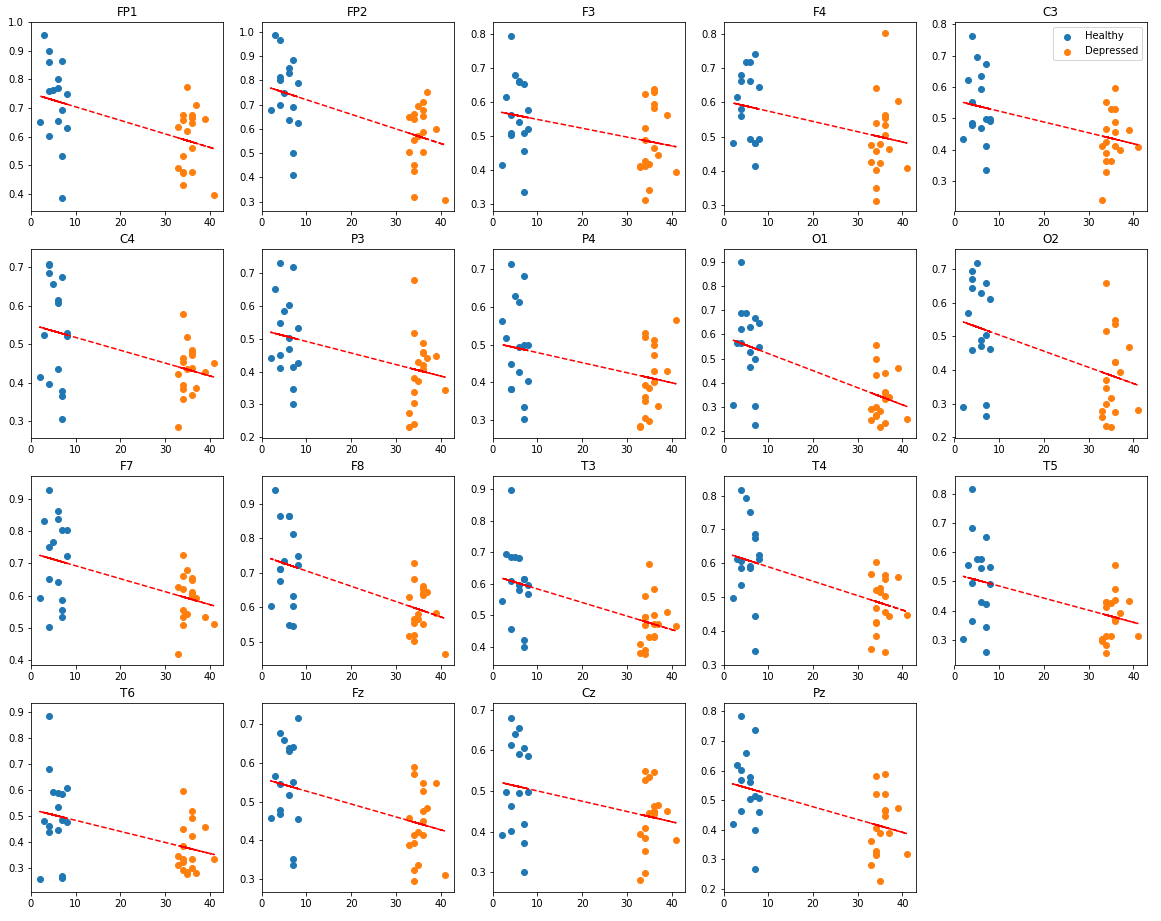
\includegraphics[width=1\textwidth]{./Images/dists/dfadepcorr.png} }
  \caption{Trend of values of largest Lyapunov exponent as a function of depression score. The correlation is significantly ($p$ < 0.05) positive for all channels with exception of FP1, FP2, F3, C3, C4, F7, F8, T3.}
\end{figure}

\begin{table}[tbp]
\centering
\tiny
  \parbox{.49\linewidth}{
\begin{tabular}{|c|c|c|c|c|}
\hline
\textbf{Channel} & \textbf{Depressed} & \textbf{Healthy} & \textbf{p-value} & \textbf{Sig.} \\ \hline
mean     & 0.503 $\pm$ 0.104 & 0.561 $\pm$ 0.125 & 0.027 & *     \\ \hline
std      & 0.109 $\pm$ 0.032 & 0.105 $\pm$ 0.025 & 0.681 &       \\ \hline
FP1      & 0.637 $\pm$ 0.144 & 0.694 $\pm$ 0.154 & 0.168 &       \\ \hline
FP2      & 0.641 $\pm$ 0.166 & 0.710 $\pm$ 0.169 & 0.131 &       \\ \hline
F3       & 0.520 $\pm$ 0.131 & 0.553 $\pm$ 0.134 & 0.153 &       \\ \hline
F4       & 0.527 $\pm$ 0.127 & 0.566 $\pm$ 0.125 & 0.104 &       \\ \hline
C3       & 0.500 $\pm$ 0.128 & 0.528 $\pm$ 0.126 & 0.183 &       \\ \hline
C4       & 0.474 $\pm$ 0.105 & 0.535 $\pm$ 0.132 & 0.049 & *     \\ \hline
P3       & 0.442 $\pm$ 0.148 & 0.487 $\pm$ 0.149 & 0.100 &       \\ \hline
P4       & 0.435 $\pm$ 0.127 & 0.479 $\pm$ 0.141 & 0.135 &       \\ \hline
O1       & 0.401 $\pm$ 0.144 & 0.507 $\pm$ 0.178 & 0.011 & *     \\ \hline
O2       & 0.437 $\pm$ 0.155 & 0.503 $\pm$ 0.155 & 0.076 &       \\ \hline
F7       & 0.627 $\pm$ 0.131 & 0.695 $\pm$ 0.159 & 0.035 & *     \\ \hline
F8       & 0.624 $\pm$ 0.129 & 0.694 $\pm$ 0.155 & 0.014 & *     \\ \hline
T3       & 0.527 $\pm$ 0.119 & 0.580 $\pm$ 0.146 & 0.057 &       \\ \hline
T4       & 0.516 $\pm$ 0.119 & 0.595 $\pm$ 0.130 & 0.007 & **    \\ \hline
T5       & 0.436 $\pm$ 0.151 & 0.493 $\pm$ 0.141 & 0.088 &       \\ \hline
T6       & 0.421 $\pm$ 0.140 & 0.482 $\pm$ 0.138 & 0.066 &       \\ \hline
Fz       & 0.471 $\pm$ 0.111 & 0.528 $\pm$ 0.130 & 0.053 &       \\ \hline
Cz       & 0.469 $\pm$ 0.094 & 0.518 $\pm$ 0.119 & 0.040 & *     \\ \hline
Pz       & 0.453 $\pm$ 0.140 & 0.521 $\pm$ 0.150 & 0.051 &       \\ \hline
\end{tabular}
\subcaption{DFA}
}
\hfill
  \parbox{.49\linewidth}{
\begin{tabular}{|c|c|c|c|c|}
\hline
\textbf{Channel} & \textbf{Depressed} & \textbf{Healthy} & \textbf{p-value} & \textbf{Sig.} \\ \hline
mean     & 0.557 $\pm$ 0.079 & 0.592 $\pm$ 0.095 & 0.051 &       \\ \hline
std      & 0.080 $\pm$ 0.027 & 0.068 $\pm$ 0.022 & 0.038 & *     \\ \hline
FP1      & 0.638 $\pm$ 0.102 & 0.669 $\pm$ 0.096 & 0.139 &       \\ \hline
FP2      & 0.649 $\pm$ 0.117 & 0.668 $\pm$ 0.113 & 0.554 &       \\ \hline
F3       & 0.565 $\pm$ 0.086 & 0.585 $\pm$ 0.103 & 0.250 &       \\ \hline
F4       & 0.576 $\pm$ 0.091 & 0.603 $\pm$ 0.098 & 0.189 &       \\ \hline
C3       & 0.562 $\pm$ 0.090 & 0.576 $\pm$ 0.107 & 0.293 &       \\ \hline
C4       & 0.548 $\pm$ 0.074 & 0.574 $\pm$ 0.102 & 0.163 &       \\ \hline
P3       & 0.513 $\pm$ 0.121 & 0.538 $\pm$ 0.121 & 0.278 &       \\ \hline
P4       & 0.513 $\pm$ 0.110 & 0.542 $\pm$ 0.113 & 0.212 &       \\ \hline
O1       & 0.475 $\pm$ 0.119 & 0.554 $\pm$ 0.138 & 0.018 & *     \\ \hline
O2       & 0.499 $\pm$ 0.121 & 0.552 $\pm$ 0.123 & 0.079 &       \\ \hline
F7       & 0.650 $\pm$ 0.091 & 0.674 $\pm$ 0.103 & 0.168 &       \\ \hline
F8       & 0.643 $\pm$ 0.092 & 0.674 $\pm$ 0.118 & 0.061 &       \\ \hline
T3       & 0.587 $\pm$ 0.082 & 0.604 $\pm$ 0.103 & 0.332 &       \\ \hline
T4       & 0.571 $\pm$ 0.084 & 0.621 $\pm$ 0.091 & 0.012 & *     \\ \hline
T5       & 0.498 $\pm$ 0.112 & 0.555 $\pm$ 0.107 & 0.043 & *     \\ \hline
T6       & 0.489 $\pm$ 0.113 & 0.540 $\pm$ 0.102 & 0.038 & *     \\ \hline
Fz       & 0.537 $\pm$ 0.085 & 0.576 $\pm$ 0.100 & 0.043 & *     \\ \hline
Cz       & 0.548 $\pm$ 0.080 & 0.579 $\pm$ 0.094 & 0.063 &       \\ \hline
Pz       & 0.525 $\pm$ 0.117 & 0.567 $\pm$ 0.120 & 0.068 &       \\ \hline
\end{tabular}
\subcaption{Hurst exponent}
}
\bigskip
  \parbox{.49\linewidth}{
\begin{tabular}{|c|c|c|c|c|}
\hline
\textbf{Channel} & \textbf{Depressed} & \textbf{Healthy} & \textbf{p-value} &  \textbf{Sig.} \\ \hline
mean     & 10.144 $\pm$ 1.166 & 9.830 $\pm$ 0.884 & 0.194 &       \\ \hline
std      & 0.761 $\pm$ 0.304 & 0.662 $\pm$ 0.258 & 0.173 &       \\ \hline
FP1      & 9.650 $\pm$ 1.363 & 9.574 $\pm$ 1.122 & 0.831 &       \\ \hline
FP2      & 9.874 $\pm$ 1.387 & 9.543 $\pm$ 1.126 & 0.324 &       \\ \hline
F3       & 9.627 $\pm$ 1.260 & 9.387 $\pm$ 1.094 & 0.421 &       \\ \hline
F4       & 9.876 $\pm$ 1.421 & 9.383 $\pm$ 1.137 & 0.119 &       \\ \hline
C3       & 9.500 $\pm$ 1.234 & 9.483 $\pm$ 0.948 & 0.895 &       \\ \hline
C4       & 9.810 $\pm$ 1.302 & 9.550 $\pm$ 0.955 & 0.212 &       \\ \hline
P3       & 10.508 $\pm$ 1.060 & 10.223 $\pm$ 0.763 & 0.301 &       \\ \hline
P4       & 10.588 $\pm$ 1.051 & 10.178 $\pm$ 0.914 & 0.131 &       \\ \hline
O1       & 10.744 $\pm$ 1.380 & 10.317 $\pm$ 0.893 & 0.063 &       \\ \hline
O2       & 10.724 $\pm$ 1.394 & 10.070 $\pm$ 0.985 & 0.030 & *     \\ \hline
F7       & 9.941 $\pm$ 1.666 & 9.757 $\pm$ 1.452 & 0.657 &       \\ \hline
F8       & 9.953 $\pm$ 1.655 & 9.794 $\pm$ 1.403 & 0.543 &       \\ \hline
T3       & 9.442 $\pm$ 1.541 & 9.367 $\pm$ 1.382 & 0.742 &       \\ \hline
T4       & 9.710 $\pm$ 1.663 & 9.422 $\pm$ 1.357 & 0.375 &       \\ \hline
T5       & 10.667 $\pm$ 1.211 & 10.240 $\pm$ 1.027 & 0.107 &       \\ \hline
T6       & 10.877 $\pm$ 1.226 & 10.165 $\pm$ 0.948 & 0.017 & *     \\ \hline
Fz       & 10.296 $\pm$ 1.171 & 10.098 $\pm$ 0.851 & 0.349 &       \\ \hline
Cz       & 10.284 $\pm$ 1.038 & 9.972 $\pm$ 0.754 & 0.243 &       \\ \hline
Pz       & 10.663 $\pm$ 1.140 & 10.254 $\pm$ 0.902 & 0.200 &       \\ \hline
\end{tabular}
\subcaption{Largest Lyapunov exponent}
}
\hfill
  \parbox{.49\linewidth}{
\begin{tabular}{|c|c|c|c|c|}
\hline
\textbf{Channel} & \textbf{Depressed} & \textbf{Healthy} & \textbf{p-value} & \textbf{Sig.} \\ \hline
mean     & 0.768 $\pm$ 0.141 & 0.796 $\pm$ 0.103 & 0.119 &       \\ \hline
std      & 0.087 $\pm$ 0.045 & 0.085 $\pm$ 0.045 & 0.870 &       \\ \hline
FP1      & 0.819 $\pm$ 0.172 & 0.834 $\pm$ 0.150 & 0.611 &       \\ \hline
FP2      & 0.788 $\pm$ 0.169 & 0.839 $\pm$ 0.138 & 0.135 &       \\ \hline
F3       & 0.819 $\pm$ 0.170 & 0.848 $\pm$ 0.141 & 0.264 &       \\ \hline
F4       & 0.801 $\pm$ 0.182 & 0.851 $\pm$ 0.145 & 0.115 &       \\ \hline
C3       & 0.835 $\pm$ 0.158 & 0.830 $\pm$ 0.118 & 0.793 &       \\ \hline
C4       & 0.807 $\pm$ 0.172 & 0.823 $\pm$ 0.106 & 0.119 &       \\ \hline
P3       & 0.715 $\pm$ 0.111 & 0.733 $\pm$ 0.089 & 0.257 &       \\ \hline
P4       & 0.702 $\pm$ 0.115 & 0.736 $\pm$ 0.108 & 0.148 &       \\ \hline
O1       & 0.701 $\pm$ 0.146 & 0.729 $\pm$ 0.111 & 0.066 &       \\ \hline
O2       & 0.705 $\pm$ 0.146 & 0.753 $\pm$ 0.127 & 0.016 & *     \\ \hline
F7       & 0.803 $\pm$ 0.202 & 0.815 $\pm$ 0.178 & 0.681 &       \\ \hline
F8       & 0.802 $\pm$ 0.216 & 0.815 $\pm$ 0.174 & 0.421 &       \\ \hline
T3       & 0.862 $\pm$ 0.208 & 0.869 $\pm$ 0.177 & 0.634 &       \\ \hline
T4       & 0.835 $\pm$ 0.218 & 0.860 $\pm$ 0.169 & 0.230 &       \\ \hline
T5       & 0.714 $\pm$ 0.134 & 0.748 $\pm$ 0.097 & 0.030 & *     \\ \hline
T6       & 0.694 $\pm$ 0.115 & 0.747 $\pm$ 0.092 & 0.008 & **    \\ \hline
Fz       & 0.744 $\pm$ 0.132 & 0.768 $\pm$ 0.098 & 0.218 &       \\ \hline
Cz       & 0.749 $\pm$ 0.113 & 0.782 $\pm$ 0.082 & 0.079 &       \\ \hline
Pz       & 0.696 $\pm$ 0.117 & 0.736 $\pm$ 0.117 & 0.131 &       \\ \hline
\end{tabular}
\subcaption{Sample entropy}
}
\bigskip
\parbox{.49\linewidth}{
\begin{tabular}{|c|c|c|c|c|}
\hline
\textbf{Channel} & \textbf{Depressed} & \textbf{Healthy} & \textbf{p-value} &  \textbf{Sig.} \\ \hline
mean     & 1.357 $\pm$ 0.139 & 1.402 $\pm$ 0.113 & 0.082 &       \\ \hline
std      & 0.095 $\pm$ 0.043 & 0.091 $\pm$ 0.042 & 0.793 &       \\ \hline
FP1      & 1.423 $\pm$ 0.186 & 1.456 $\pm$ 0.177 & 0.450 &       \\ \hline
FP2      & 1.396 $\pm$ 0.188 & 1.459 $\pm$ 0.163 & 0.123 &       \\ \hline
F3       & 1.413 $\pm$ 0.177 & 1.459 $\pm$ 0.157 & 0.173 &       \\ \hline
F4       & 1.396 $\pm$ 0.181 & 1.462 $\pm$ 0.153 & 0.094 &       \\ \hline
C3       & 1.435 $\pm$ 0.149 & 1.448 $\pm$ 0.125 & 0.693 &       \\ \hline
C4       & 1.401 $\pm$ 0.147 & 1.436 $\pm$ 0.111 & 0.097 &       \\ \hline
P3       & 1.299 $\pm$ 0.115 & 1.336 $\pm$ 0.104 & 0.194 &       \\ \hline
P4       & 1.291 $\pm$ 0.108 & 1.336 $\pm$ 0.120 & 0.111 &       \\ \hline
O1       & 1.265 $\pm$ 0.141 & 1.322 $\pm$ 0.123 & 0.035 & *     \\ \hline
O2       & 1.273 $\pm$ 0.146 & 1.338 $\pm$ 0.129 & 0.031 & *     \\ \hline
F7       & 1.406 $\pm$ 0.190 & 1.437 $\pm$ 0.173 & 0.301 &       \\ \hline
F8       & 1.402 $\pm$ 0.198 & 1.447 $\pm$ 0.173 & 0.153 &       \\ \hline
T3       & 1.448 $\pm$ 0.188 & 1.468 $\pm$ 0.174 & 0.532 &       \\ \hline
T4       & 1.427 $\pm$ 0.214 & 1.452 $\pm$ 0.147 & 0.243 &       \\ \hline
T5       & 1.281 $\pm$ 0.126 & 1.334 $\pm$ 0.106 & 0.035 & *     \\ \hline
T6       & 1.258 $\pm$ 0.113 & 1.330 $\pm$ 0.093 & 0.004 & ***   \\ \hline
Fz       & 1.335 $\pm$ 0.152 & 1.375 $\pm$ 0.124 & 0.148 &       \\ \hline
Cz       & 1.352 $\pm$ 0.123 & 1.411 $\pm$ 0.098 & 0.040 & *     \\ \hline
Pz       & 1.287 $\pm$ 0.126 & 1.334 $\pm$ 0.123 & 0.131 &       \\ \hline
\end{tabular}
\subcaption{Higuchi fractal dimension}
}
\hfill
  \parbox{.49\linewidth}{
\begin{tabular}{|c|c|c|c|c|}
\hline
\textbf{Channel} & \textbf{Depressed} & \textbf{Healthy} & \textbf{p-value} & \textbf{Sig.} \\ \hline
mean     & 10.892 $\pm$ 0.681 & 10.734 $\pm$ 0.723 & 0.332 &       \\ \hline
std      & 0.667 $\pm$ 0.166 & 0.629 $\pm$ 0.161 & 0.393 &       \\ \hline
FP1      & 11.439 $\pm$ 0.814 & 11.067 $\pm$ 1.058 & 0.076 &       \\ \hline
FP2      & 11.405 $\pm$ 0.921 & 11.141 $\pm$ 0.998 & 0.522 &       \\ \hline
F3       & 11.100 $\pm$ 0.881 & 10.673 $\pm$ 0.809 & 0.076 &       \\ \hline
F4       & 10.888 $\pm$ 0.884 & 10.844 $\pm$ 0.947 & 0.870 &       \\ \hline
C3       & 10.481 $\pm$ 0.872 & 10.289 $\pm$ 0.895 & 0.375 &       \\ \hline
C4       & 10.495 $\pm$ 0.880 & 10.402 $\pm$ 0.978 & 0.706 &       \\ \hline
P3       & 10.665 $\pm$ 0.854 & 10.419 $\pm$ 0.861 & 0.301 &       \\ \hline
P4       & 10.465 $\pm$ 0.766 & 10.313 $\pm$ 0.774 & 0.460 &       \\ \hline
O1       & 11.002 $\pm$ 1.225 & 11.023 $\pm$ 0.944 & 0.646 &       \\ \hline
O2       & 10.990 $\pm$ 1.022 & 10.894 $\pm$ 1.020 & 0.657 &       \\ \hline
F7       & 10.979 $\pm$ 0.799 & 10.842 $\pm$ 0.837 & 0.402 &       \\ \hline
F8       & 11.116 $\pm$ 1.020 & 10.858 $\pm$ 0.835 & 0.358 &       \\ \hline
T3       & 11.133 $\pm$ 0.763 & 11.085 $\pm$ 0.946 & 0.974 &       \\ \hline
T4       & 11.256 $\pm$ 0.924 & 11.090 $\pm$ 0.965 & 0.565 &       \\ \hline
T5       & 10.988 $\pm$ 0.927 & 10.970 $\pm$ 0.995 & 0.961 &       \\ \hline
T6       & 11.038 $\pm$ 0.729 & 10.911 $\pm$ 0.743 & 0.588 &       \\ \hline
Fz       & 10.614 $\pm$ 0.792 & 10.322 $\pm$ 0.877 & 0.206 &       \\ \hline
Cz       & 10.444 $\pm$ 1.047 & 10.545 $\pm$ 0.962 & 0.767 &       \\ \hline
Pz       & 10.454 $\pm$ 0.959 & 10.254 $\pm$ 0.886 & 0.384 &       \\ \hline
\end{tabular}
\subcaption{Correlation dimension}
}
\caption{Comparison of mean values of measures computed for depressed and healthy patients.}
\end{table}


\subsection{Low and high remission}
\info[inline]{There was no control group given no drugs. Each patient assigned different treatment. Each patient started on different level of depression. We recognize this is inherently bad study design.}

\section{Classification}
We used two classifiers: logistic regression (LR) and support vector machine (SVM). One third of randomly selected samples was held out as a test set, the rest was used for training and cross validation. Feature selection was performed on LR with regularization strength 1 and SVM with regularization strenth 1 and linear kernel (i.e. $k(\vec{x_1}, \vec{x_2}) = \vec{x_1} \cdot \vec{x_2}$) using
\begin{itemize}
  \item recursive feature elimination with 3-fold cross validation based on coefficients of the linear model,
  \item elimination of features with below-mean coefficients of the linear model,
  \item selection of 5 features with the highest $\chi^2$ statistics between values of the feature and corresponding class,\unsure{Am I justified in using $\chi^2$?}
  \item genetic algorithm with 3-fold cross validation (scoring models based on ROC AUC, population size 50, 50 generations, crossover probability 0.8, mutation probability 0.2, and tournament size 5).
\end{itemize}
Then, a brute force grid search with 3-fold cross validation was performed on each classifier to select 
\begin{itemize}
  \item the optimal regularization stength, and norm for LR, and
  \item the optimal regularization strength and kernel type (linear, polynomial, or radial basis function with coefficients $\gamma = 1/n_f$, where $n_f$ is the number of selected features) for SVM.\unsure{Am I justified in changing the kernel type?}
\end{itemize}
These classifiers were evaluated on the test set. The best performing classifiers (based on accuracy, precision, recall, f-score, ROC AUC and confusion matrices) for each measure were selected, and then manually optimized by adding, removing, or replacing features based on differences in distributions described in Section \ref{sec:distanal}, performance of similar classifiers on similar measures, and results of other studies. In some cases, hyperparameters were modified. The results are described in the following text.

\subsection{Depression}

\begin{table}[tbp]
\centering
\begin{tabular}{|c|c|c|c|c|c|c|}
\hline
\textbf{Measure} & \textbf{Class.} & \textbf{Acc.} & \textbf{F-sc.} & \textbf{ROC AUC} & \textbf{CM} & \textbf{Channels} \\ \hline
DFA & LR & 0.88 & 0.88 & 0.91 & $\left( \begin{smallmatrix} 9 & 2 \\ 0 & 6 \end{smallmatrix} \right)$ & C3, C4, O1, T4 \\ \hline 
HE & LR & 0.76 & 0.77 & 0.78 & $\left( \begin{smallmatrix} 8 & 3 \\ 1 & 5 \\ \end{smallmatrix} \right)$ & O1, T4 \\ \hline
CD & SVM (poly.) & 0.76 & 0.76 & 0.74 & $\left( \begin{smallmatrix} 9 & 2 \\ 2 & 4\end{smallmatrix} \right)$ & F3, F4, P3, O1, T4, T5, Cz, Pz \\ \hline
LLE & SVM (lin.) & 0.71 & 0.71 & 0.77 & $\left( \begin{smallmatrix} 6 & 5 \\ 0 & 6 \end{smallmatrix} \right)$ & FP1, FP2, F4, C3, O1, T3, T6 \\ \hline
SE & LR & 0.71 & 0.71 & 0.73 & $\left( \begin{smallmatrix} 7 & 4 \\ 1 & 5 \end{smallmatrix} \right)$ & P3, P4, T5, T6 \\ \hhline{=|=|=|=|=|=|=}
DFA & SVM (rbf) & 0.70 & 0.70 & 0.72 & $\left( \begin{smallmatrix} 8 & 7 \\ 1 & 11 \end{smallmatrix} \right)$ & O1, T5, T6 \\ \hline
CD & SVM (rbf) & 0.70 & 0.70 & 0.71 & $\left( \begin{smallmatrix} 10 & 5 \\ 3 & 9 \end{smallmatrix} \right)$ & C4, P4, T4, T6, Cz \\ \hline
HE & LR & 0.70 & 0.70 & 0.70 & $\left( \begin{smallmatrix} 11 & 4 \\ 4 & 8 \end{smallmatrix} \right)$ & F3, F4, T3, T5, Fz, Cz \\ \hline
\end{tabular}
\caption{Evaluation of depression classification. The first part corresponds to classifiers trained on 15 healthy (DS $\leq$ 10) and 24 depressed (DS $\geq$ 30) patients. The second part corresponds to classifiers trained on 24 healthy (DS $\leq$ 12) and 36 depressed (DS $\geq$ 32). Both before and after treatment sessions are included.}
\label{tab:depcl}

\bigskip

\begin{tabular}{|c|c|c|c|c|c|c|}
\hline
\textbf{Measure} & \textbf{Class.} & \textbf{Acc.} & \textbf{F-sc.} & \textbf{ROC AUC} & \textbf{CM} & \textbf{Channels} \\ \hline
CD & SVM (rbf) & 1.00 & 1.00 & 1.00 & $\left( \begin{smallmatrix} 10 & 0 \\ 0 & 10 \end{smallmatrix} \right)$ & F4, C4, O1, F7, F8, T5, T6 \\ \hline
LLE & LR & 0.80 & 0.80 & 0.80 & $\left( \begin{smallmatrix} 9 & 1 \\ 3 & 7 \end{smallmatrix} \right)$ & \small{FP2, F3, F4, P3, P4, F7, F8, T6, Fz, Cz} \\ \hline
DFA & LR & 0.80 & 0.80 & 0.80 & $\left( \begin{smallmatrix} 8 & 2 \\ 2 & 8 \end{smallmatrix} \right)$ & FP2, F3, O1, T5, T6, Cz \\ \hline
HE & LR & 0.70 & 0.70 & 0.70 & $\left( \begin{smallmatrix} 7 & 3 \\ 3 & 7 \end{smallmatrix} \right)$ & FP2, F3, O1, T5, T6, Cz \\ \hhline{=|=|=|=|=|=|=}
LLE & SVM (rbf) & 0.76 & 0.76 & 0.77 & $\left( \begin{smallmatrix} 16 & 7 \\ 3 & 16 \end{smallmatrix} \right)$ & F3, F4, O1, O2, T6, Fz \\ \hline
HE & LR & 0.71 & 0.71 & 0.73 & $\left( \begin{smallmatrix} 14 & 9 \\ 3 & 16 \end{smallmatrix} \right)$ & P3, F7, T4, T6, Cz \\ \hline
CD & LR & 0.69 & 0.69 & 0.70 & $\left( \begin{smallmatrix} 14 & 9 \\ 4 & 15 \end{smallmatrix} \right)$ & F4, C4, T5 \\ \hline
HD & LR & 0.69 & 0.69 & 0.70 & $\left( \begin{smallmatrix} 13 & 10 \\ 3 & 16 \end{smallmatrix} \right)$ & FP2 \\ \hline
DFA & LR & 0.64 & 0.64 & 0.64 & $\left( \begin{smallmatrix} 15 & 8 \\ 7 & 12 \end{smallmatrix} \right)$ & C3, P4, F7, T6 \\ \hline
\end{tabular}
\caption{Evaluation of remission. The first part corresponds to split of the whole dataset according to the first and last septiles of $m_2 / m_1$ (considered non-remitting and remitting patients respectively). The second part corresponds to split according to first and last terciles of $m_2 / m_1$. Both before and after treatment sessions are included.}
\label{tab:respcl}
\end{table}

\subsection{Remission}

\chapter{Machine learning approach}

\chapter*{Conclusion}

\bibliographystyle{plain}
\bibliography{refs}
\end{document}
